% Template for a Computer Science Tripos Part II project dissertation
\documentclass[12pt,a4paper,twoside,openright]{report}
\usepackage[pdfborder={0 0 0}]{hyperref}    % turns references into hyperlinks
\usepackage[left=25mm, right=25mm, bottom=25mm, top=20mm]{geometry}  % adjusts page layout
\usepackage{karnaugh-map}
\usepackage{tikz}
\usepackage{graphicx}  % allows inclusion of PDF, PNG and JPG images
\usepackage{bm}
\usepackage{listings}
\usepackage{titlesec}
\usepackage{subcaption}
\usepackage{array}
\usepackage{verbatim}
\usepackage{mathdots}
\usepackage{amsfonts}
\usepackage{amssymb}
\usepackage{xcolor}
\usepackage{placeins}
\usepackage{amsthm}
\usepackage{amsmath}
\usepackage{tabu}
\usepackage{docmute}   % only needed to allow inclusion of proposal.tex
\usepackage[utf8]{inputenc}
\usepackage{mathtools}
\usepackage{changepage}
\usepackage{url}
\usepackage{blindtext}
\usepackage{tabularx,booktabs}
\usepackage{dirtree}
\usepackage{cite}
\usepackage{float} % Prevent Latex from repositioning tables
\usepackage{graphicx}
% \usepackage{listings}

\lstset{
  language=Haskell,
  basicstyle=\linespread{1}\ttfamily\footnotesize,
  keywordstyle=\color{blue},
  commentstyle=\color{gray}\textit,
  stringstyle=\color{orange},
  showstringspaces=false,
  breaklines=true,
  % frame=lines,
  rulecolor=\color{gray},
  % numbers=left,
  % numberstyle=\tiny\color{gray},
  xleftmargin=2em,
  framexleftmargin=1.5em,
  aboveskip=1em,
  belowskip=1em,
  escapeinside={(*}{*)},
  captionpos=b
}

% lstset{
%   language=Haskell,
%   basicstyle=\ttfamily\small,
%   breaklines=true,
%   frame=single,
%   numbers=left,
%   numberstyle=\tiny\color{gray},
%   showstringspaces=false
% }

%--- Remove hbox warning
\hfuzz=5000.002pt 
%----------------------------------------------------------------------------------------

% Formatting Commands
\newcommand{\keyword}[1]{\textbf{#1}}
\newcommand{\tabhead}[1]{\textbf{#1}}
\newcommand{\code}[1]{\texttt{#1}}
\newcommand{\file}[1]{\texttt{\bfseries#1}}
\newcommand{\option}[1]{\texttt{\itshape#1}}

%----------------------------------------------------------------------------------------
%% *****************************************************************
\newlength{\upBranch} % shift up the text  lines <<<<
\setlength{\upBranch}{0.7ex} % 

\newlength{\tolineSpace} % blank space bellow text  lines  <<<
\setlength{\tolineSpace}{1mm}% 

\usepackage{xpatch} % needed <<<<<<<<
\makeatletter

\DeclareMathOperator*{\argmax}{arg\,max}
\DeclareMathOperator*{\argmin}{arg\,min}

\xpatchcmd{\dirtree} % root
{\vbox{\@nameuse{DT@body@1}}}
{\raisebox{-\tolineSpace}{\vbox{\@nameuse{DT@body@1}}}}
{}{}    

\xpatchcmd{\dirtree} % below space
{\advance\dimen\z@ by-\@nameuse{DT@lastlevel@\the\DT@countiv}\relax}
{\advance\dimen\z@ by-\tolineSpace \advance\dimen\z@ by-\@nameuse{DT@lastlevel@\the\DT@countiv}\relax}
{}{}
    
\xpatchcmd{\dirtree}% shift up the text  lines
{\kern\DT@sep\box\z@\endgraf}
{\kern\DT@sep\raisebox{-\upBranch}{\box\z@}\endgraf}
{}{}    

\makeatother
%% *****************************************************************

\titleformat{\chapter}
  % {\normalfont\Large\bfseries}{\thesection}{1em}{}
{\normalfont\huge\bfseries}{}{}{\Huge}[{\titlerule[0.8pt]}]
%-----
% Language setting
\usepackage[english]{babel}
%\raggedbottom                           % try to avoid widows and orphans
\sloppy
\clubpenalty1000%
\widowpenalty1000%

\renewcommand{\baselinestretch}{1.1}    % adjust line spacing to make
                                        % more readable


\theoremstyle{definition}
\newtheorem{definition}{Definition}[section]

\graphicspath{{figs/}}

\begin{document}

% Change these

\newcommand{\mcandidate}{2200D}
\newcommand{\mfullname}{Judah Daniels}
\newcommand{\mcollege}{Clare College}
\newcommand{\mtitle}{Inferring Harmony from Free Polyphony}
\newcommand{\ntitle}{Inferring Harmony from Free Polyphony}
\newcommand{\mexamination}{Computer Science Tripos -- Part II}
\newcommand{\mdate}{July, 2023}
\newcommand{\moriginator}{Christoph Finkensiep}
\newcommand{\msupervisor}{Dr Peter Harrison}
\newcommand{\mwordcount}{5434}
\newcommand{\mlinecount}{2272}
% Consent to the dissertation made available to University members
\newcommand{\mconsent}{I am content for my dissertation to be made available to the students and staff of the University.}
% For the Declaration of originality
\newcommand{\msignature}{Judah Daniels}


\bibliographystyle{acm}


\setlength{\parskip}{10pt}
\setlength{\parindent}{0pt}

%%%%%%%%%%%%%%%%%%%%%%%%%%%%%%%%%%%%%%%%%%%%%%%%%%%%%%%%%%%%%%%%%%%%%%%%
% Title
%%%%%%%%%%%%%%%%%%%%%%%%%%%%%%%%%%%%%%%%%%%%%%%%%%%%%%%%%%%%%%%%%%%%%%%%

\thispagestyle{empty}

\rightline{\LARGE \textbf{\mfullname}}

\vspace*{60mm}
\begin{center}
\Huge
\textbf{\mtitle} \\[5mm]
\mexamination \\[5mm]
\mcollege \\[5mm]
\mdate  % today's date
\end{center}

%%%%%%%%%%%%%%%%%%%%%%%%%%%%%%%%%%%%%%%%%%%%%%%%%%%%%%%%%%%%%%%%%%%%%%%%%%%%%%
% Proforma, table of contents and list of figures
%%%%%%%%%%%%%%%%%%%%%%%%%%%%%%%%%%%%%%%%%%%%%%%%%%%%%%%%%%%%%%%%%%%%%%%%%%%%%%

\pagestyle{plain}

\newpage
\newpage
\section*{Declaration of originality}

I, \mfullname{} of \mcollege, being a candidate for Part II of the Computer Science Tripos, hereby declare that this dissertation and the work described in it are my own work, unaided except as may be specified below, and that the dissertation does not contain material that has already been used to any substantial extent for a comparable purpose. \mconsent

\bigskip
\leftline{Signed \msignature}
\bigskip
\leftline{Date \today}

\chapter*{Proforma}

% \hbadness=0

{\large
  \begin{tabular}{ll}
Candidate Number:   & \bf \mcandidate                   \\
Project Title:      & \bf \mtitle                       \\
Examination:        & \bf \mexamination, \mdate         \\
Word Count:         & \bf \mwordcount\footnotemark[1]   \\
Code Line Count:    & \bf \mlinecount\footnotemark[2]   \\
Project Originator: & \bf \moriginator                  \\
Supervisor:         & \bf \msupervisor                  \\ 
\end{tabular}
}

\footnotetext[1]{This word count was computed
by \texttt{texcount main.tex}
}
\footnotetext[2]{This code line count was computed
by using \texttt{cloc}
}
\stepcounter{footnote}

\section*{Original Aims of the Project}
% The original aim was to implement a parsing algorithm for symbolic music, using the derivation to infer the underlying harmonic structure, then explore data driven approaches for heuristic design.


\section*{Work Completed}



\section*{Special Difficulties}
There were no special difficulties encountered in this project

\newpage
{
\renewcommand{\baselinestretch}{0.75}\normalsize
\tableofcontents
\renewcommand{\baselinestretch}{1.0}\normalsize
}
\listoffigures

\newpage
\section*{Acknowledgements}
I'd like to thank Christoph Finkensiep and Peter Harrison for being awesome.



%%%%%%%%%%%%%%%%%%%%%%%%%%%%%%%%%%%%%%%%%%%%%%%%%%%%%%%%%%%%%%%%%%%%%%%
% now for the chapters

\pagestyle{headings}

\chapter{Introduction}
% \textit{This dissertation explores efficient search strategies for parsing symbolic music data using a musical grammar for Automatic Chord Estimation (ACE). We first present a naive implementation of a parsing algorithm based on a recent grammatical model, then address problems of intractability through classical heuristic search methods. We will see that that my novel heuristic search algorithm achieves commendable results, providing a strong foundation for a more sophisticated automated analysis system. }

\section{Motivation and Aim}
Most of western tonal music can be described using a sequence of chords, representing a higher level harmonic structure of a piece. Automatic Chord Estimation (ACE) is the task of inferring the sequence of chords for a given piece from symbolic data. There is a small, finite set of chord types, but each chord can be realised on the musical surface in a practically infinite number of ways. Given a score $S$ (a symbolic representation of a piece of music), we wish to infer the sequence of underlying chord types $L = l_0, \dots, l_n$. 

\begin{equation}
  \begin{align}
    \hat L &= \argmax_L p(L|S) 
  \end{align}
\end{equation} 

We present a \textbf{novel solution}, the \textbf{ProtoVoice Harmony Model (PVHM)} that infers the sequence of chord types given score using probabilistic models of latent structure and harmony, dimensionality reduction, parsing strategies and heuristic search methods.

\begin{figure}[h]
  \centering
  \begin{subfigure}[t]{\textwidth}
    \centering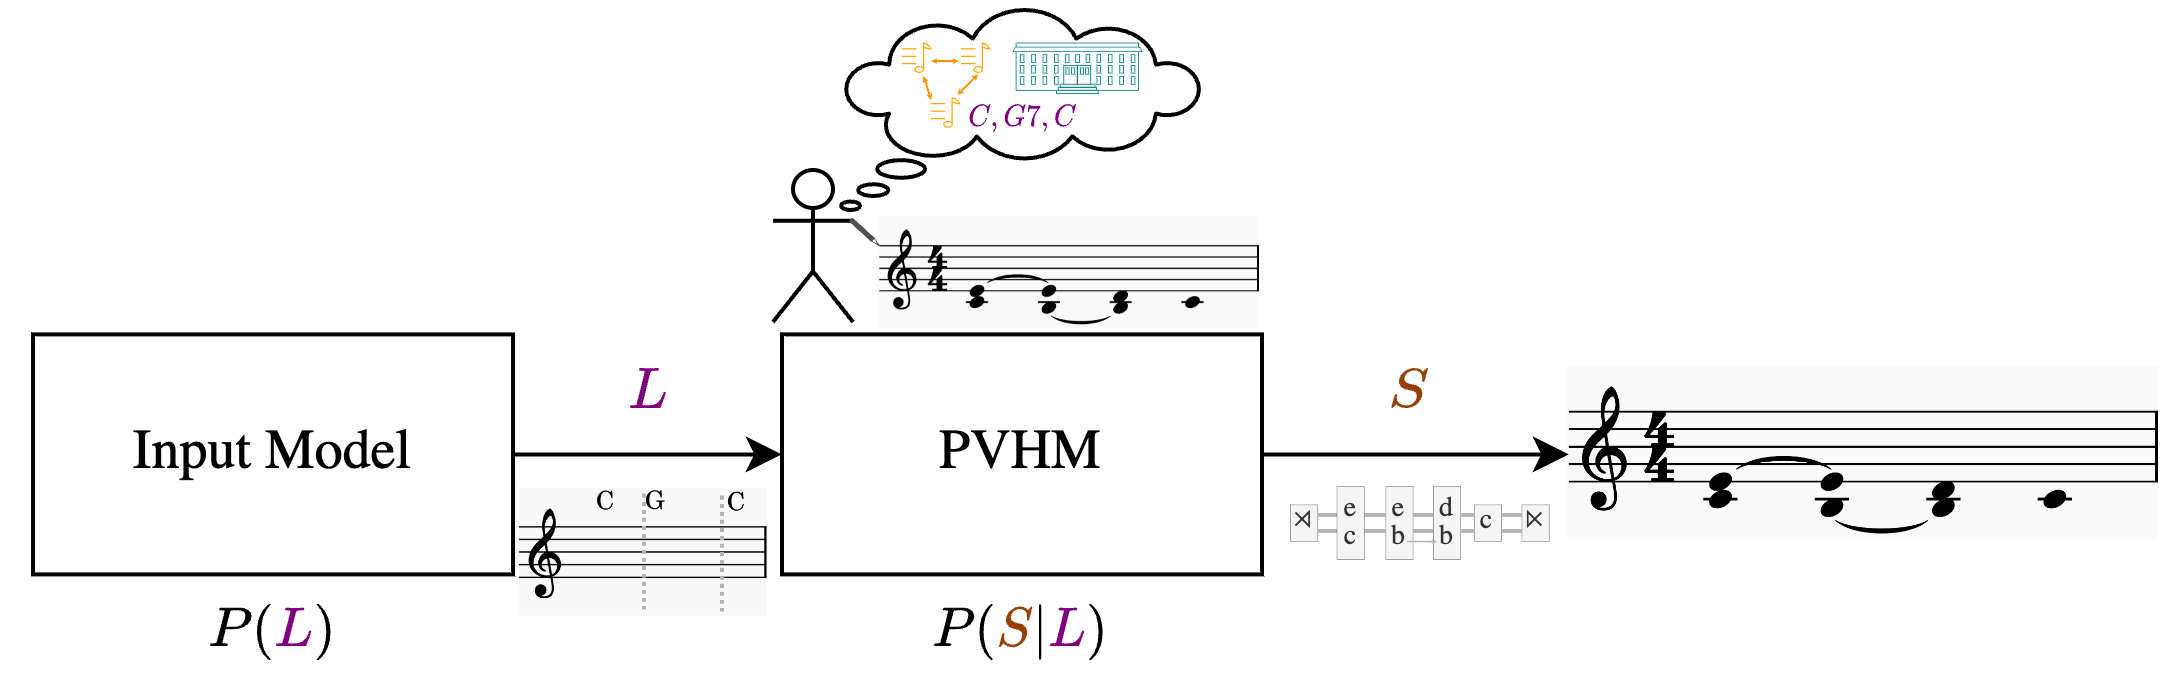
\includegraphics[keepaspectratio,width=\textwidth]{intro/overview/generation}
    \caption{Modelling}
    \label{fig:modellingOverview}
  \end{subfigure}
  \begin{subfigure}[t]{\textwidth}
    \centering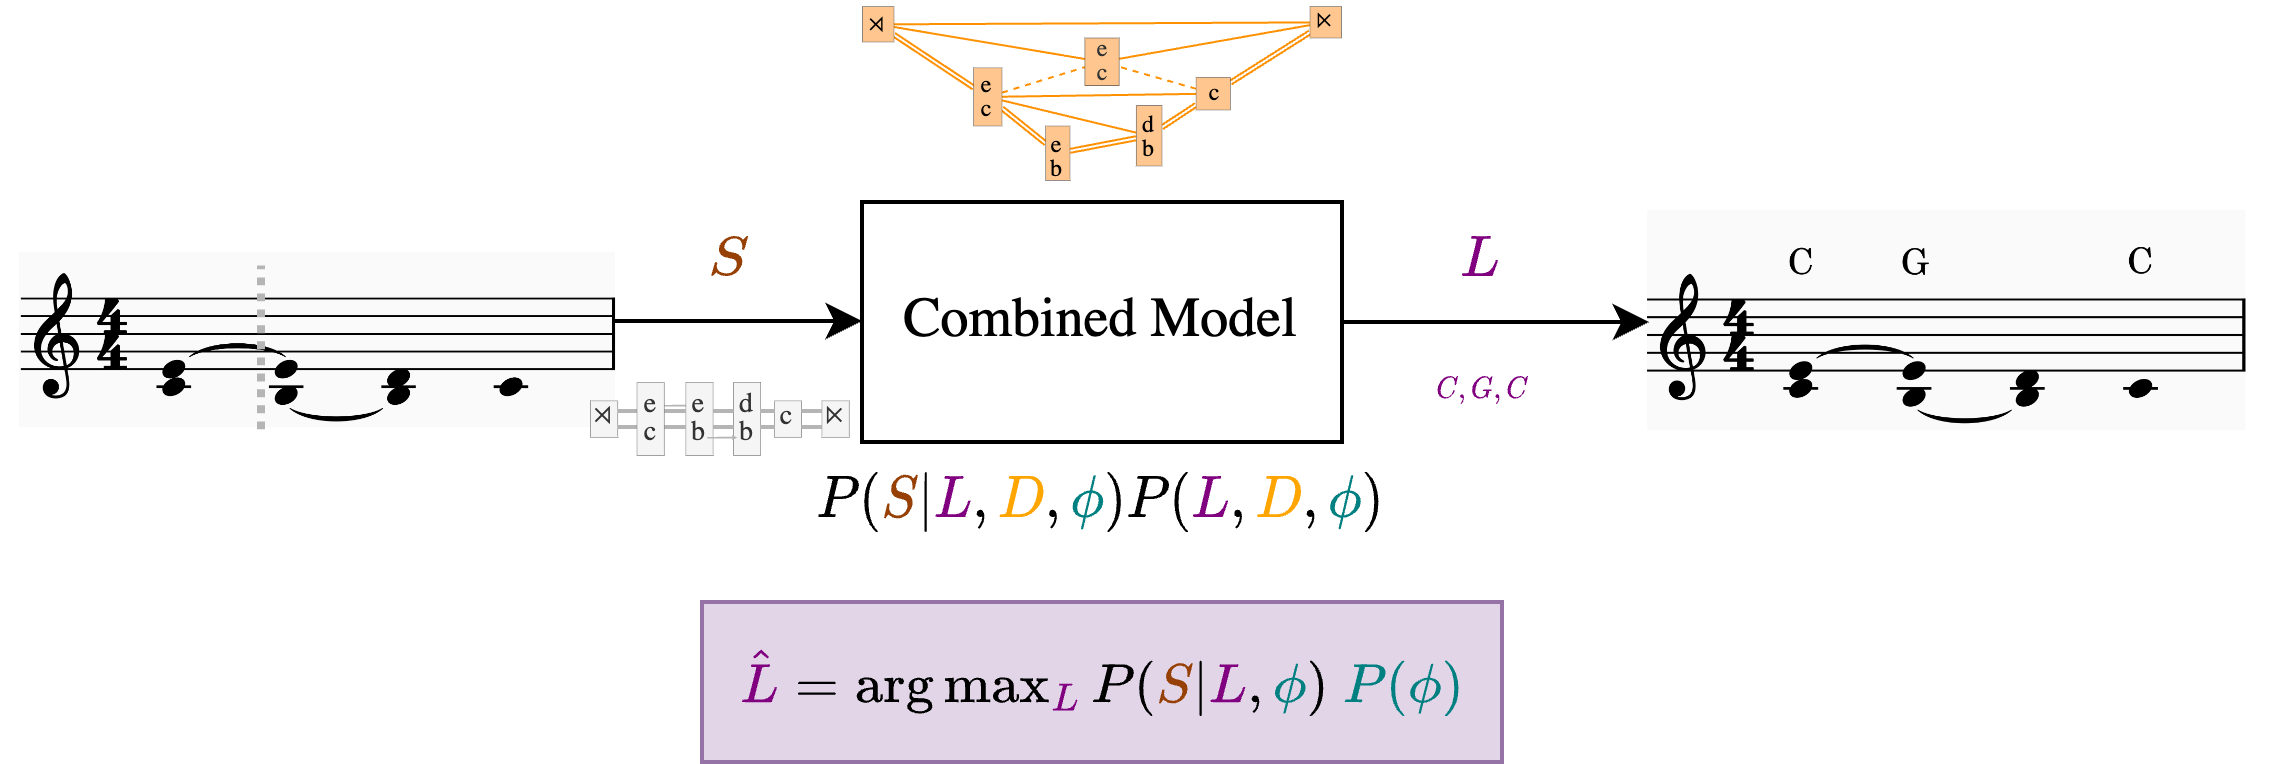
\includegraphics[keepaspectratio,width=\textwidth]{intro/overview/inference}
    \caption{Inference}
    \label{fig:inferenceOverview}
  \end{subfigure}
  \caption{Problem overview}
  \label{fig:overview}
\end{figure}


Automatic Chord Estimation has both theoretical and practical applications. 
% Novel ways to understand harmonic structure are sought after by music theorists, aiding the analysis and composition of pieces. 
Analysis of music often starts with the manual labeling each chord, which is a time consuming and cogntively demanding expert task. 
Sequences of chords provide compact representations for use in analysis, music identification and music similarity finding.
More broadly speaking, any system that involves the understanding of written tonal music will benefit from chord estimation. 

The paper \textit{Modeling and Inferring Protovoice Structure in Free Polyphony} describes a generative model that encodes the recursive and hierarchical dependencies between notes, giving rise to a grammar-like hierarchical system \cite{finkensiepModelingInferringProtovoice2021}.
This model can be used to reduce a piece into a hierarchical structure which encodes an understanding of the tonal/harmonic relations.



% Finkensiep suggests in his thesis that the protovoice model may be an effective way to infer higher level latent entities such as harmonies. Thus, in this project I will answer the question: is this model an effective way to annotate harmonies? By ‘effective’ we are referring to two things:
% \begin{itemize}
%   \item Accuracy: can the model successfully emulate how experts annotate harmonic progressions in musical passages? 
%   \item Practicality: can the model be used to do this within a reasonable time frame?
% \end{itemize}

While the original model could in theory be used to generate harmonic annotations, an exhaustive search strategy would be prohibitively time-consuming in practice for any but the shortest musical extracts; one half measure can have over 100,000 valid derivations \cite{finkensiepStructureFreePolyphony2023}. 

The \textbf{PVHM} uses \textit{heuristic search} strategies to infer \textit{latent structure} using the protovoice model, followed by \textit{feature extraction} which finally allows the chord labels to be inferred using a \textit{probabilistic model of harmony}.

\section{Related Work}

% The problem of automated chord estimation has been subject to attention since the 80s, with handcrafted grammar/rule-based being. 
Automatic chord estimation systems first emerged in in the 60's, making use of handcrafted grammar/rule-based systems \cite{maxwellExpertSystemHarmonizing1992} \cite{winogradLinguisticsComputerAnalysis1968}, followed by the development of optimisation algorithms in the early 2000s \cite{pardoAlgorithmsChordalAnalysis2002}. In more recent years, supervised learning approaches have have risen in popularity, exploiting large datasets and improved compute power \cite{niEndtoendMachineLearning2011} \cite{mcleodModularSystemHarmonic2021} \cite{masadaChordRecognitionSymbolic2018}. 
\par 
The protovoice model is the first to provide a unified theory that relates three aspects of tonal music analysis that are typically considered independently: voice-leading, how notes relate to each other \textit{sequentially}; harmony, how notes relate to each other through \textit{simulataneity}; and note function, how notes relate to each other through recursive \textit{functional dependencies}. Previous models have been developed alongside parsing algorithms to perform automatic chord estimation that consider these dimensions of musical structure separately \cite{maxwellExpertSystemHarmonizing1992} \cite{winogradLinguisticsComputerAnalysis1968}, but in this project we use the relationship between these dimensions of music as the basis of heuristic design.
\par
% Distinction to be drawn between approaches that take segmented or non-segmented pieces. Some models make use of a joint segmentation and labelling approach \cite{masadaChordRecognitionSymbolic2018}. 

\section{Achievements}

This was an ambitious project; I met all the Success Criteria and completed the extension tasks. I show that the protovoice model can be used to effectively annotate pieces with chord labels, and these results provide a promising foundation for the model being developed further as a sophisticated tool for the automated analysis of western total music. The PVHM has been made \textbf{open source} to accommodate future research in the area.


%%%%%%%%%%%%%%%%%%%%%%%%%%%%%%%%%%%%%%%%%%%%%%%%%%%%%%%%%%%%%%%%%%%%%
% Preparation
%%%%%%%%%%%%%%%%%%%%%%%%%%%%%%%%%%%%%%%%%%%%%%%%%%%%%%%%%%%%%%%%%%%%%

\chapter{Preparation}
% \textit{In this chapter, I present the work which was undertaken before the code was written. I first provide an exposition of the Protovoice Model which forms the foundation of this project, describing how it can be used to infer harmony. Subsequently, I discuss probabilistic programming and Bayesian inference, including a probabilistic model of harmony. Finally, I describe the software engineering techniques and principles used throughout the project. }

\section{Bayesian Inference}
\subsection{Bayesian Inference and Modelling}

\textbf{Bayesian inference} is a statistical inference paradigm in which Bayes' theorem is used to update the probability for a hypothesis in light of available evidence. This allows us to \textit{infer} information about \textit{latent}(hidden) variables based on \textit{observed} evidence.

The method of Bayesian inference reduces to representing the \textit{joint distribution} of all the random variables in a system, such that we can compute any probability of interest in that system. Let $X$ and $Z$ denote the observed and latent(unobserved) variables respectively, and let $Y$ denote the random variable we wish to infer. 
Then we are interested in representing the \textit{joint distribution} $P(X,Y,Z)$. \textbf{Modelling} is the process of approximating a joint distribution through abstract representations and relationships.

We first consider how we would compute the best hypothesis for $Y$ given the evidence $X$, ignoring the latent variables $Z$.
% In order to infer information about the value of $Y$ given the joint distribution $P(X,Y)$ and the observation $X$, we consider the \textit{conditional} probability distribution, $P(Y|X)$. 

There are two methods used to find the most likely hypothesis $Y$:
\begin{itemize}
  \item  The \textbf{maximum a priori estimate} maximises the \textit{conditional likelihood} of the hypothesis given the evidence, given by $P(Y|X)$. This requires us to know the \textit{prior} $P(Y)$, the distribution of the hypothesis, beforehand. The prior can be learned from labeled data.
    \begin{equation}
      \begin{align}
        \hat{Y} &= \argmax_Y P(Y|X) \\
                &= \argmax_Y P(X|Y)P(Y)
      \end{align}
      \label{eq:map}
    \end{equation}
  \item  The \textbf{maximum likelihood estimate} maximises the conditional likelihood of the observed evidence given the hypothesis, given by $P(X|Y)$. This method allows us to capture \textit{uncertainty} in the prediction, given by $P(X|\hat{Y})$. 
    \begin{equation}
      \hat{Y} = \argmax_Y P(X|Y)
      \label{eq:mle}
    \end{equation}
\end{itemize}

\begin{definition}[Factoring]
\begin{equation}
  P(A,B) = P(B|A)~P(A)
  \label{eq:bayesRule}
\end{equation}
\end{definition}

\begin{definition}[Marginalisation]
\begin{equation}
  P(A) = \sum\limits_B P(A|B)~P(B)
  \label{eq:marginalisation}
\end{equation}
\end{definition}

\begin{definition}[Chain Rule of Probability]
\begin{equation}
  P(A,B) = P(A|B)~P(B)
  \label{eq:chainRule}
\end{equation}
\end{definition}

\subsection{Inferring Latent variables}
To incorporate the latent variables $Z$, we use \textit{marginalisation} and the \textit{chain rule of probability} to show that: 
\begin{equation}
  \begin{align*}
    P(Y|X) &= \sum\limits_Z P(Y,Z|X) \\
           &= \sum\limits_Z P(Y|X,Z)~P(Z|X) 
  \end{align*}
  \label{eq:}
\end{equation}

Given a model of $P(Z|X)$, we avoid summing over the values of $Z$ by approximating $\hat{Z} = \argmax_Z P(Z|X) $, the most likely value of $Z$ given $X$, using MLE or MAP estimation.

We thus update the prior $P(Z|X)$ as follows:
\[P(Z|X) = \begin{cases} 1 &\text{if } Z=\hat{Z} \\ 0 &\text{otherwise}\end{cases}\]

This gives us an approximation of $P(Y|X)$:

\begin{equation}
  P(Y|X) &\approx P(Y|X,\hat{Z}) 
  \label{eq:inferenceTrick}
\end{equation}

\section{Overview of Approach}

\textbf{Probabilistic programming} is a programming paradigm that makes use of
model definitions and statistical inference algorithms to compute the
conditional distribution of inputs that could have given rise to an observed
output. 

In the context of ACE, we consider the underlying sequence of chord labels $L_0, L_1,\dots L_n$ as an \textbf{input}, and the musical surface or score as the \textbf{observed output} $S$. 

In this sense, ACE can be solved by finding the most likely sequence of labels for the given surface, described by the equation: 

\begin{equation}
  \hat L = \argmax_L P\left(L|S\right)
  \label{eq:aceProbSol}
\end{equation}

The difficulty arises from the complexity and prohibitively large number of the \textbf{latent variables} $\bm{ \phi }$; in reality, we need to maximise $\sum\limits_{\bm{\phi}}P(L|S,\bm{ \phi })~P(\bm{\phi}|S)$.

\begin{equation}
  \hat L = \argmax_L \sum\limits_{\bm{\phi}} P(L | S,\bm{\phi})~P(\bm{\phi}|S)
  \label{eq:aceProbSolLatent}
\end{equation}

The set of latent variables $\bm{\phi}$ is \textbf{practically infinite}. These include the author's compositional conception, their musical conception, cognitive phenomena experienced by listeners, shared experience distilled into music theory, musical trends/culture and notational conventions. 

This cannot be solved analytically, but we approximate $\hat{L}$ using models that encode domain specific knowledge about both the music generation and labelling processes, through joint conditional distributions. 

\subsubsection{Approximating Conditional Likelihood with MLE}

Now consider the set of latent RVs $\bm{\phi}$ as the union of two \textit{disjoint sets}, $\bm{\phi'}$ and $\bm{\phi''}$, where $\bm{\phi'}$ is the subset of $\bm{\phi}$ which we can \textit{reasonably infer} given $L$ and $S$, and $\bm{\phi''} = \bm{\phi} \setminus \bm{\phi}'$. Assuming $P(\bm{\phi'} | L)$ and $P(\bm{\phi''} | L)$ are independent, it follows:

\begin{equation}
  \begin{align}
    P(L|S) &= \sum\limits_{\bm{\phi'}}\sum\limits_{\bm{\phi''}} P(L | S,\bm{\phi'},\bm{ \phi'' })~P(\bm{ \phi' }, \bm{ \phi'' } |S) \\
           &= \sum\limits_{\bm{\phi'}}\sum\limits_{\bm{\phi''}} P(L | S,\bm{\phi'},\bm{\phi''})~P(\bm{\phi'} | S)~P(\bm{\phi''} |S) 
  \end{align}
  % \hat L = \argmax_L \sum\limits_{\phi} P(S | L,\phi)~P(\phi|L)
  \label{eq:aceProbSolLatent}
\end{equation}

We take $P(\phi''|S)$ to be a uniform distribution as we have no prior knowledge of the latent variables that we cannot infer. 
Using the technique described in Equation~\ref{eq:inferenceTrick}, we find $\hat{\phi'}$, thus giving: 

\begin{equation}
  \begin{align}
    \hat L \approx \argmax_L P(L | S, \hat{\phi'})
  \end{align}
  % \hat L = \argmax_L \sum\limits_{\phi} P(S | L,\phi)~P(\phi|L)
  \label{eq:aceProbSolLatent}
\end{equation}








% We achieve this by only considering the latent variables $\phi'$ that we can reasonably \textit{infer}, discarding the rest of $\phi$ by assuming $P(\phi|\phi')$ is a uniform distribution. 
% In this project, we use the protovoice model to infer the latent structure of the surface $\hat{D}$, and thus calculate $p(S|L,\hat{D})$.

% We denote the protovoice reduction transformation as $f_{pv}:(\mathcal{S}, \Phi) \to (\mathcal{S'})$.
% We then consider computing $p(S'|L;\phi)$. $S'$ is the reduced surface. In order to be able to use this transformed representation, there is a constraint that $\argmax_L p(S'|L') \approxeq \argmax_L p(S|L)$. That is, after applying the transform, the maximum likelihood estimate of the reduced surface given each sequence of labels should be the same, or as close as possible to that of the unreduced surface. In other words, the solution should be \textit{invariant} or \textit{approximately invariant} to this transformation.
\FloatBarrier
\section{Inferring Structure}
\subsection{The Protovoice Model}
The protovoice model is a formal generative model which represents a piece of music as a graph where each note is a node, and notes are connected by stepwise protovoice edges. 

The Protovoice model is primarily concerned with the analysis of Western Classical music, although it could be applied to different musical styles, such as jazz or some popular western music \cite{finkensiepStructureFreePolyphony2023}. 

\subsection{Voices}
The input we are concerned with is called a score, a symbolic abstraction of a piece of music based on a 2-dimensional axis.

The marks on on score represents notes, with the pitch of the note corresponding to its position on the vertical axis\footnote{This is a simplification as there are other factors that determine the pitch, such as the key signature, accidentals and intonation.}, and the notes' position in time represented by the horizontal axis.
\begin{figure}[h]
  \centering
  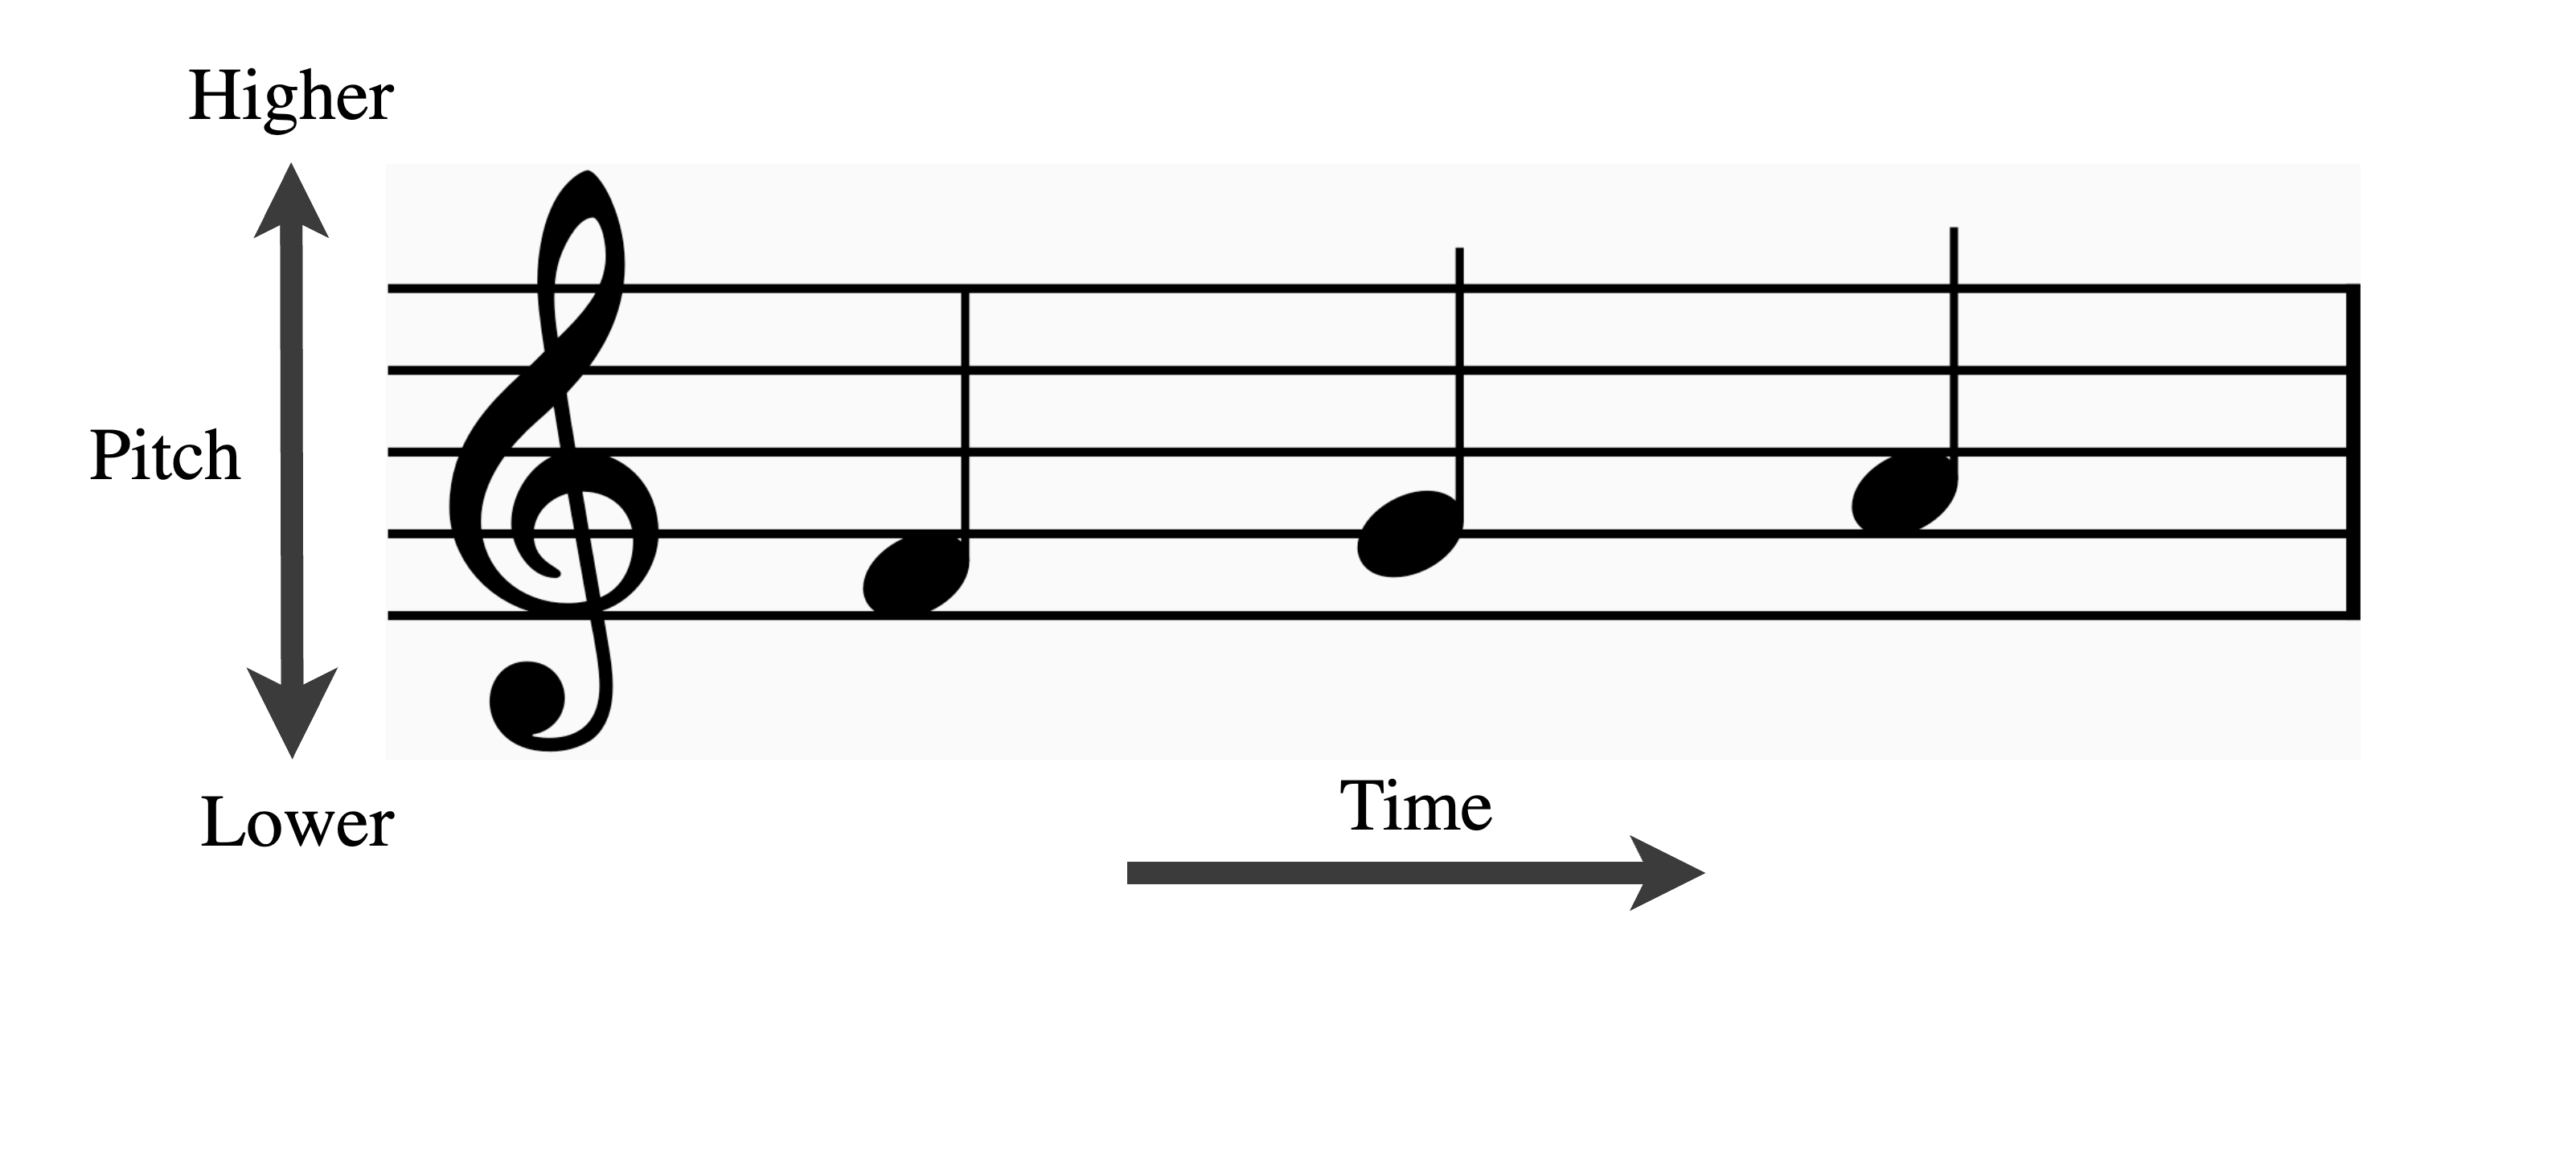
\includegraphics[width=0.55\textwidth]{prep/pitchTime.png}
  \captionsetup{width=.7\linewidth}
  \caption{An example of music notation showing an ascending stepwise sequence.}
  \label{fig:pitchTime}
\end{figure}

The notion of a \textit{voice} is crucial for the understanding of the protovoice model.
A voice typically refers to a single melodic line (sequence of notes) that is part of a musical composition.
The term is derived from its use in choral music, such as J.S Bach's four-voice chorales, which consist of 4 sung melodic lines.
The term voice is used is used more generally however, the melodic lines do not need to be sung or voice-like in character and can be performed by any melodic instrument. 


\begin{figure}[h]
  \centering
  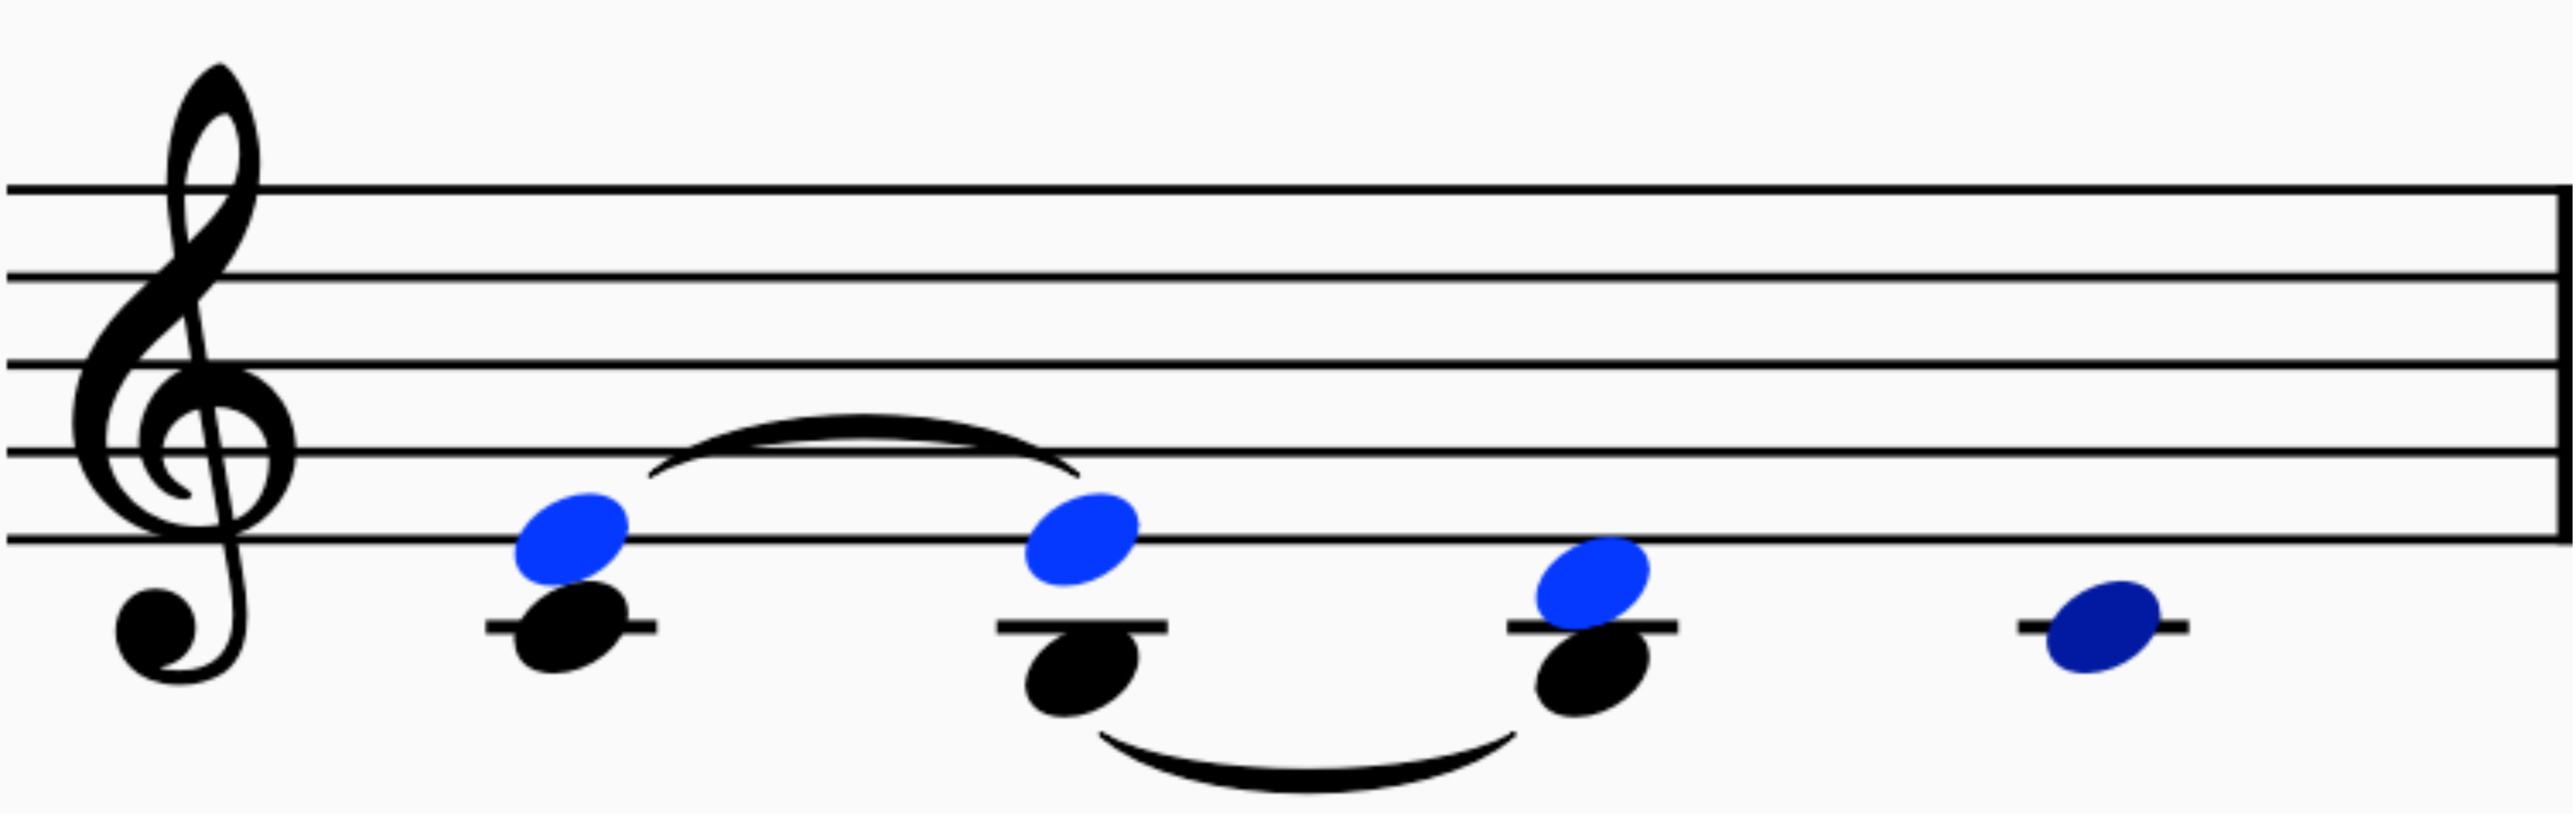
\includegraphics[width=0.45\textwidth]{prep/cadencevoices}
  \captionsetup{width=.9\linewidth}
  \caption{A short cadential phrase with two voices.}
  \label{fig:cadenceVoices}
\end{figure}

Polyphony refers to a piece of music that can contains more than one voice.
Typically polyphonic music will have a set number of voices throughout the piece, but \textit{free polyphony} refers to music where the number of voices is arbitrary and can change throughout the piece.

There are three types of relations between notes that form the basis for the protovoice model:

\begin{itemize}
  \item \textbf{Horizontal}: As music is perceived in time, natural sequential relations arise between subsequent notes, in fact, we can define a total order on the notes of a piece of music based on their positions on the horizontal axis.
  \item \textbf{Vertical}: This refers to the pitch axis on the score. The vertical(pitch) arrangement of the notes determine the emergent harmony when they are perceived simultaneously. Typically, multiple \textit{voices} heard together will lead to an emerging sequence of harmonies, which can be described using chord labels.

\begin{figure}[h]
  \centering
  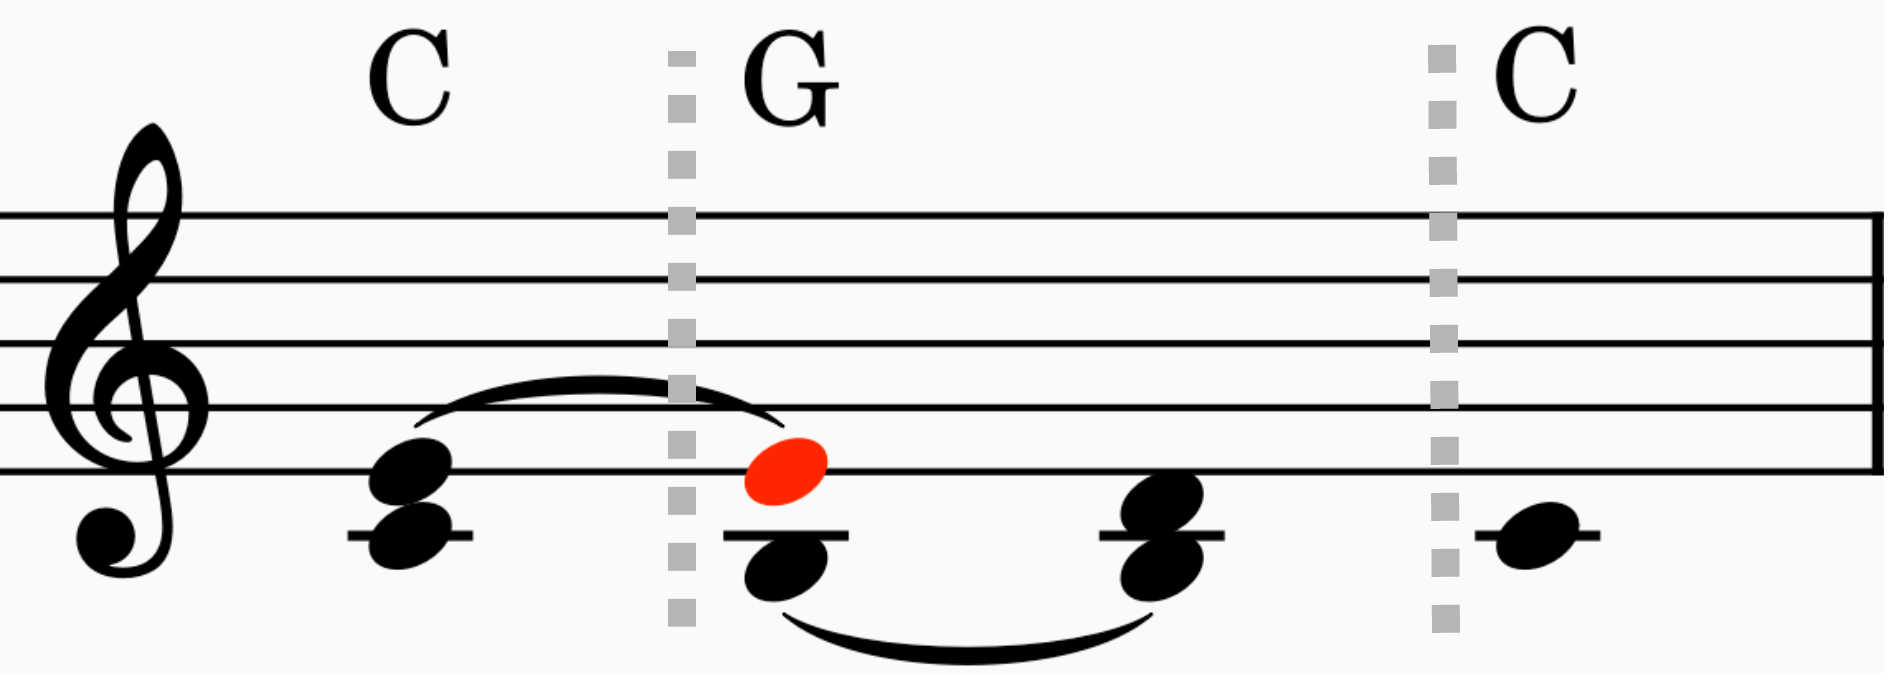
\includegraphics[width=0.45\textwidth]{prep/cadenceharmony}
  \captionsetup{width=.9\linewidth}
  \caption{Chord labels shown with segment boundaries.}
  \label{fig:cadenceHarmony}
\end{figure}

  \item \textbf{Functional}: Functional relations refer to the purpose or function of a note relative to another note. These functions can include repetitions, where both notes have the same \textit{pitch}, or ornaments/neighbour notes, where the child note is a step (single unit of pitch) away from the parent note. These relations can be applied recursively, giving rise to a network of dependencies.

\begin{figure}[h]
  \centering
  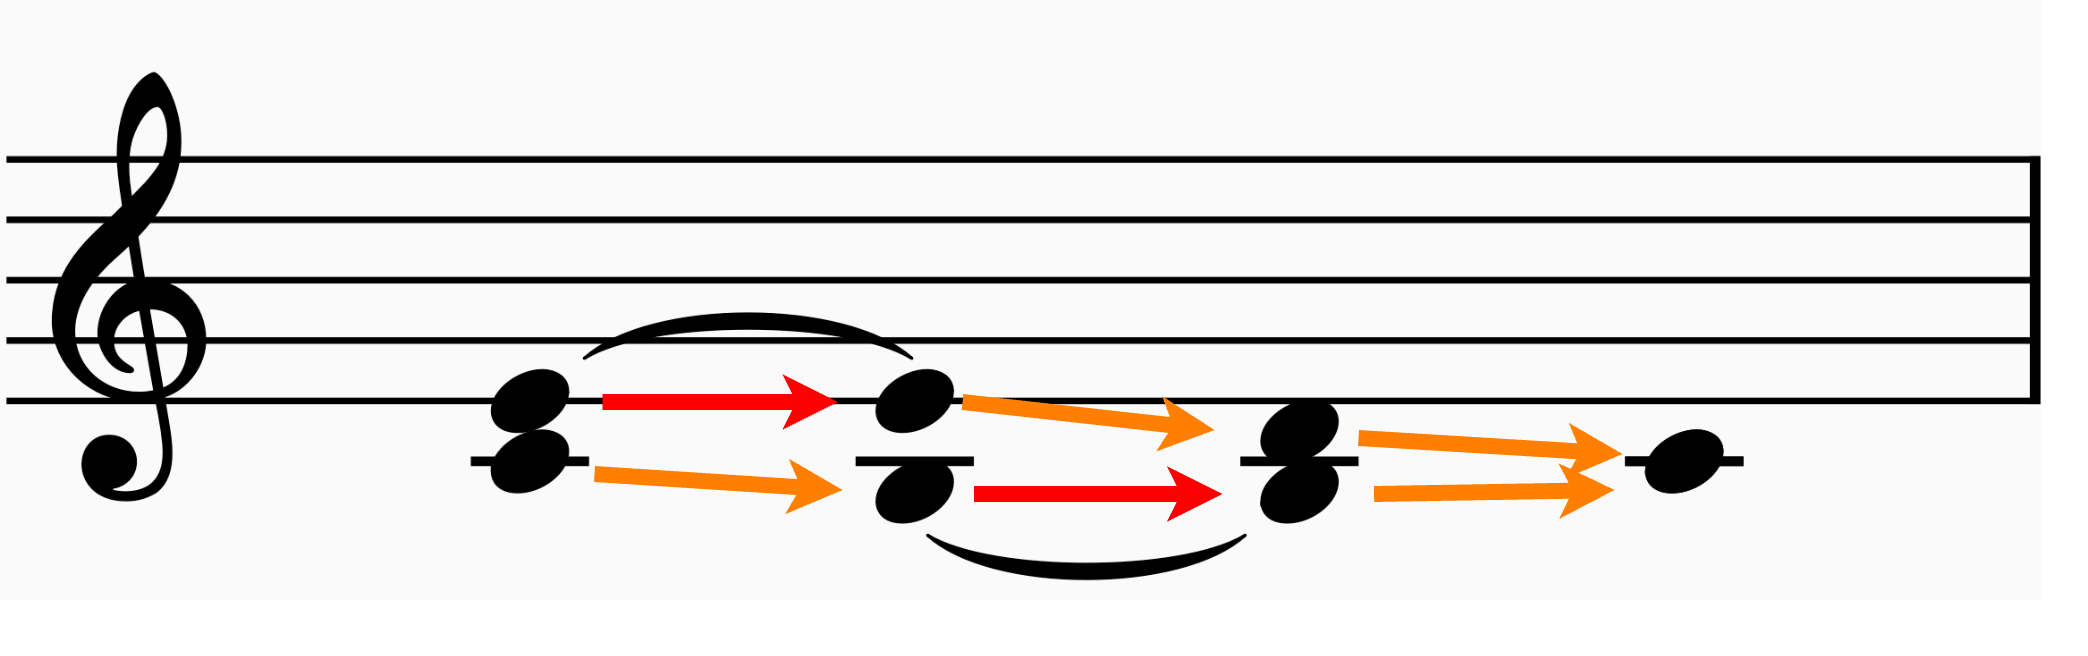
\includegraphics[width=0.45\textwidth]{prep/cadencefunctions}
  \captionsetup{width=.9\linewidth}
  \caption{Functional dependencies between notes.}
  \label{fig:cadenceFunctions}
\end{figure}

\end{itemize}

% subsection Voices (end)

\subsection{Inner Structure} % (fold)
\label{sub:Inner Structure}

Internally, the protovoice model generates a piece of music through sequential operations on notes, inserting new notes with edges connected to existing notes.

We represent protovoices as a graph $G$ with one vertex for each note, a vertex each for the beginning ($\rtimes$) and end ($\ltimes$) of the piece, and edges that indicate connections between notes.
We define a note as $p \in \mathcal{P}$ where $\mathcal{P}$ is the set of pitches, i.e the set of vertical positions on the score\footnote{See Appendix C for a detailed explaination of the pitch representation used in this project}. 
A \textit{protovoice} is a path within this graph.

\par 
The protovoice model is characterised by 3 primitive generative operations on notes.

\begin{itemize}
  % \setlength\itemsep{1em}
  \item \textbf{Repetitions:} a note of the same pitch is repeated before or after a given note
  \item \textbf{Neighbor notes:} a stepwise ornament to a note. 
  \item \textbf{Passing notes:} notes connecting two protovoices that are separated by a larger interval.
\end{itemize}

These operations relate notes to one or two \textit{parent} notes, which we can describe as rules. Operations on a single parent are represented by attaching a new \textit{child} note with an edge connected to a parent note: 
\begin{equation}
  p \implies x \to p \text{~~~~or~~~~} p \implies p \to x 
  \label{eq:singlesidedinnerop}
\end{equation}
Operations with two parents are represented by edge replacement. 
\begin{equation}
  p_1 \to p_2 ~~~\implies~~ p_1 \to c \to p_2 \label{edge replacement}
  \label{eq:doublesidedinnerop}
\end{equation}

The generation of a piece begins with the empty piece ($\rtimes \to \ltimes$) and involves the recursive application of inner operations, or rules. The full set of rules is left to the appendix, but here are a few as an example:
\begin{equation}
  \begin{align}
    x &\implies n \to x && \text{\texttt{left-neighbor}}
  \label{eq:leftNeighbor} \\
    \rtimes \to \ltimes &\implies \rtimes \to x \to \ltimes && \text{\texttt{root-note}}
  \label{eq:rootNote} \\
    x \to y &\implies x \to x' \to y && \text{\texttt{repeat-after'}}
  \label{eq:repeatAfter}\\
  \end{align} 
\end{equation}
% subsection Inner Structure (end)
\subsection{Outer Structure}
\label{sub:Outer Structure}

The inner structure provided by protovoices captures the sequential and functional organisation of notes, but does not capture when notes are simultaneous. To model simulataneity of notes we introduce \textit{slices}, representing segments of a piece where a group of notes are heard, and \textit{transitions} which contain the protovoice edges between notes in the two neighbouring slices. These provide a higher level abstraction that are used to capture more musical structure. 
\par
As slices and transitions contain notes and edges respectively, we call the slices and transitions \textit{outer structure}, and the notes and edges contained therein \textit{inner structure}.

\begin{definition}[Multiset] A \textit{multiset} is a set that allows multiple instances for each of its elements, formally defined as an ordered pair $(A,m)$ where $A$ is the \textit{underlying set} of the multiset, and $m:A \to \mathbb{Z}^+$ gives the \textit{multiplicity}, such that the number of occurences of $a$ in $(A,m)$ is given by $m(a)$. 
\end{definition}

\begin{definition}[Slice] A \textit{slice} $s \in \mathcal{S}$ is defined as a multiset of pitches $(\mathcal{P}, m)$. 
\begin{equation}
  s = \left\{ p_1^{m(p_1)} , \dots, p_n^{m(p_n)} \right\}  
  \label{eq:sliceDef}
\end{equation}
\end{definition}

\begin{definition}[Transition] A \textit{transition} $t \in \mathcal{T}$ relates two adjacent slices, $s_l$ and $s_r$, with a configuration of edges $e$. 
  \begin{equation}
    \begin{align}
      $t = (s_l, e, s_r)$ 
    \end{align}
    \label{eq:biPath}
  \end{equation}
\end{definition}

The slices and transitions form a graph given slices as nodes and transitions as edges (containing inner edges). However as transitions only relate sequentially adjacent slices, the outer structure is in fact a \textit{path graph} and can thus be represented as a list of vertices.

\begin{definition}[Path Graph] \footnote{This is refered to as a \texttt{Path} in the source code} A \textit{path graph} is a graph which can be represented as an alternating sequence of elements from two sets $A$ and $B$, defined inductively as:
  \begin{equation}
    \begin{align}
      P &= a     &&&& a \in A \\
      P &= abP   &&&& a \in A, b \in B 
    \end{align}
    \label{eq:biPath}
  \end{equation}
\end{definition}

\begin{definition}[Outer Structure] ~\\The \textit{outer structure} is thus defined as a path graph, represented as:
\begin{equation}
    \begin{align}
      P = t_1~s_1~t_2~s_2~\dots~t_n     &&&& t_i \in \mathcal{T},~s_i \in \mathcal{S},~ i \in 1\dots n \\
    \end{align}
  \label{eq:outerStructureDef}
\end{equation}
\end{definition}

The outer structure is generated by applying three operations described as production rules recursively:

\begin{itemize}
  \item A \textbf{split} replaces a transition $t$ by inserting a new slice $s'$ and two surrounding transitions $t_l$ and $t_r$. Each of the edges in $t$ can have by one or more inner operations applied to it. The edges generated by these inner operations can either be discarded, or keep to form the new edges of $t_l$ and $t_r$.
\begin{equation}
  t \to t'_l~s'~t'_r
  \label{eq:splitrule}
\end{equation}
  \item A \textbf{spread} replaces a slice $s$ by distributing its notes to two child slices $s'_l$ and $s'_r$. 
\begin{equation}
  t_l~s~t_r \to t'_l~s'_l~t'_m~s'_r~t'_r
  \label{eq:spreadrule}
\end{equation}
\item A \textbf{freeze} marks a transition as terminal, such that the edges within the transition can no longer have operations applied to it. 
\begin{equation}
  t \to \underline{t}
  \label{eq:freezerule}
\end{equation}
\end{itemize}

\begin{figure}[h]
  \centering
  \begin{subfigure}[t]{.28\textwidth}
    \centering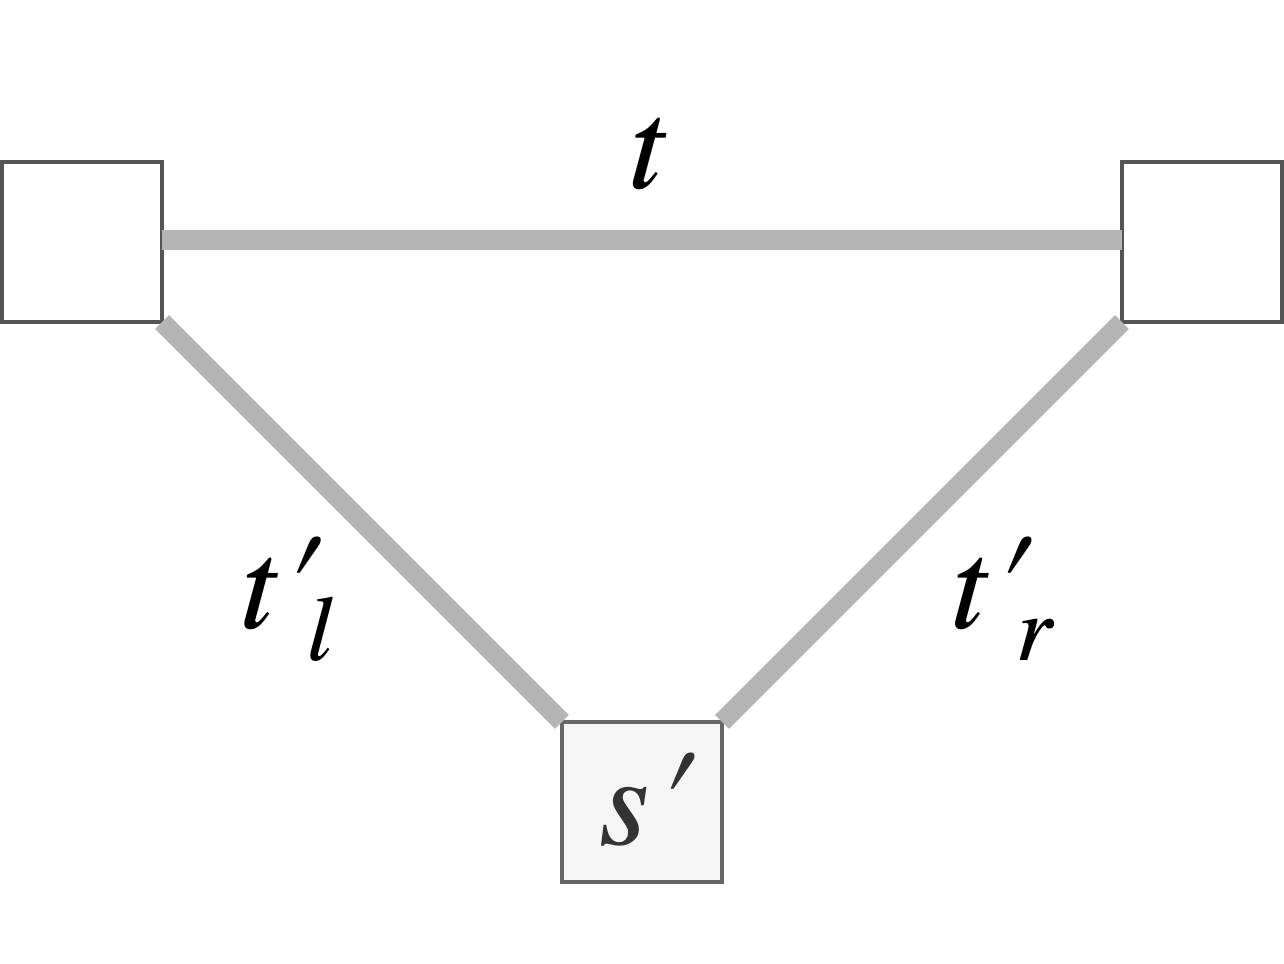
\includegraphics[keepaspectratio,width=\textwidth]{prep/outer/split}
    \caption{\texttt{split}}
    \label{fig:splitOp}
  \end{subfigure}
  \begin{subfigure}[t]{.46\textwidth}
    \centering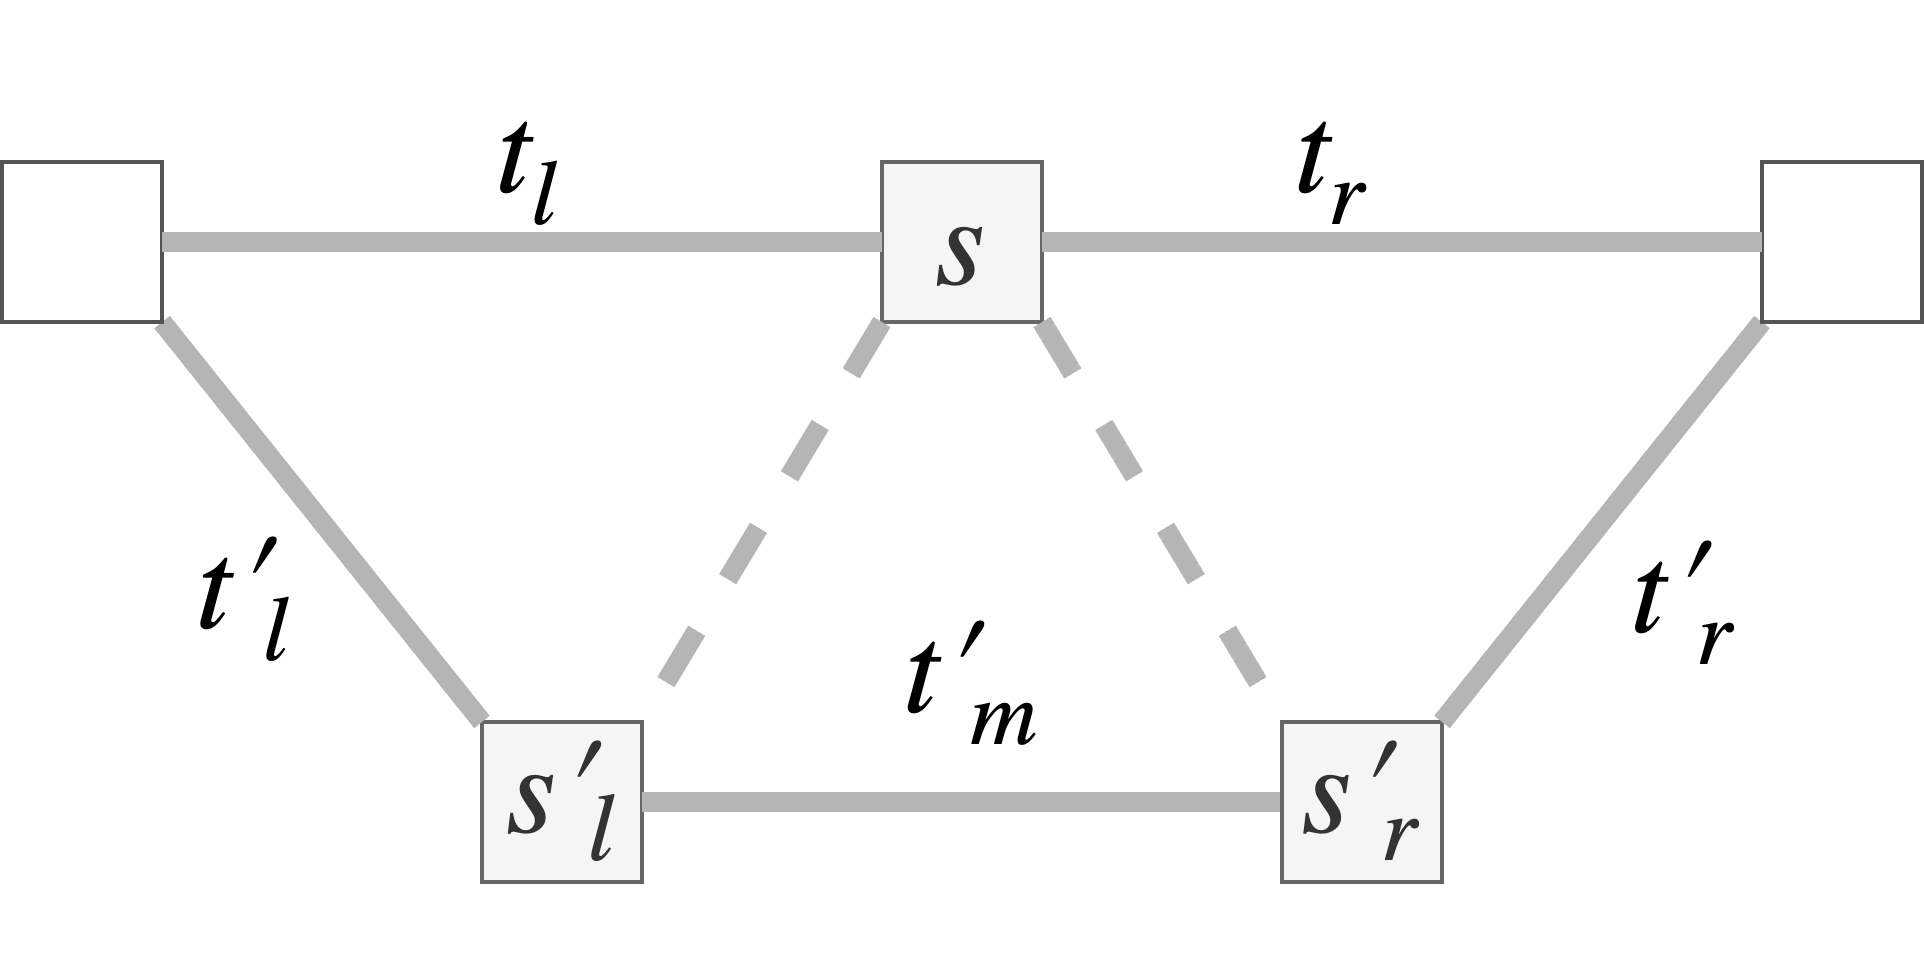
\includegraphics[keepaspectratio,width=0.91\textwidth]{prep/outer/spread}
    \caption{\texttt{spread}}
    \label{fig:spreadOP}
  \end{subfigure}
  \begin{subfigure}[t]{.24\textwidth}
    \centering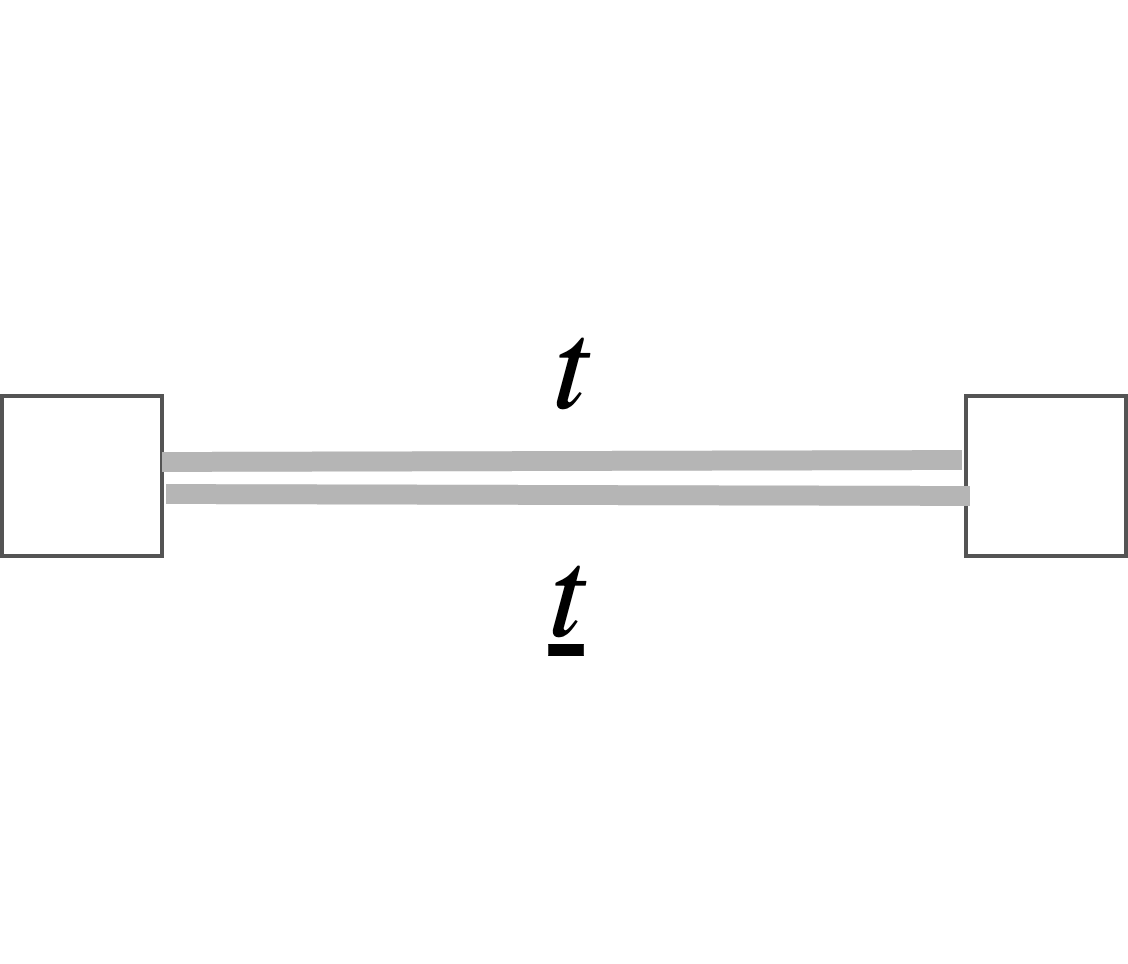
\includegraphics[keepaspectratio,width=\textwidth]{prep/outer/freeze}
    \caption{\texttt{freeze}}
    \label{fig:freezeOp}
  \end{subfigure}
  \centering
  \captionsetup{width=.9\linewidth}
  \caption{The three operations on outer structure. }
  \label{fig:outerOperations}
\end{figure}

Figure~\ref{fig:outerOperations} shows a diagrammatic representation of each of these operations. The original slices and transitions are shown at the top of each diagram, while the lower part shows the generated structure after each outer operation is applied.

The generation of a piece thus begins with the empty transition $t_0$, followed by a \texttt{split} operation, which generates the root slice of the piece. 

Figure~\ref{fig:innerOuterStructure} gives an example derivation of the short phrase shown in Figure~\ref{fig:cadenceVoices}. In Figure~\ref{fig:cadenceOuterDer}, we can see that 4 outer operations have been applied to generate the surface. The spread operation introduces a passing edge between e and c, shown as the dashed line in Figure~\ref{fig:cadenceInnerDer}. Note that the vertically aligned notes in Figure~\ref{fig:cadenceInnerDer} correspond to the notes in the surface slices in Figure~\ref{fig:cadenceOuterDer}, and the final surface shown on the right of Figure~\ref{fig:cadenceDerivation}.
\begin{figure}[h]
  \centering
  \begin{subfigure}[t]{.55\textwidth}
    \centering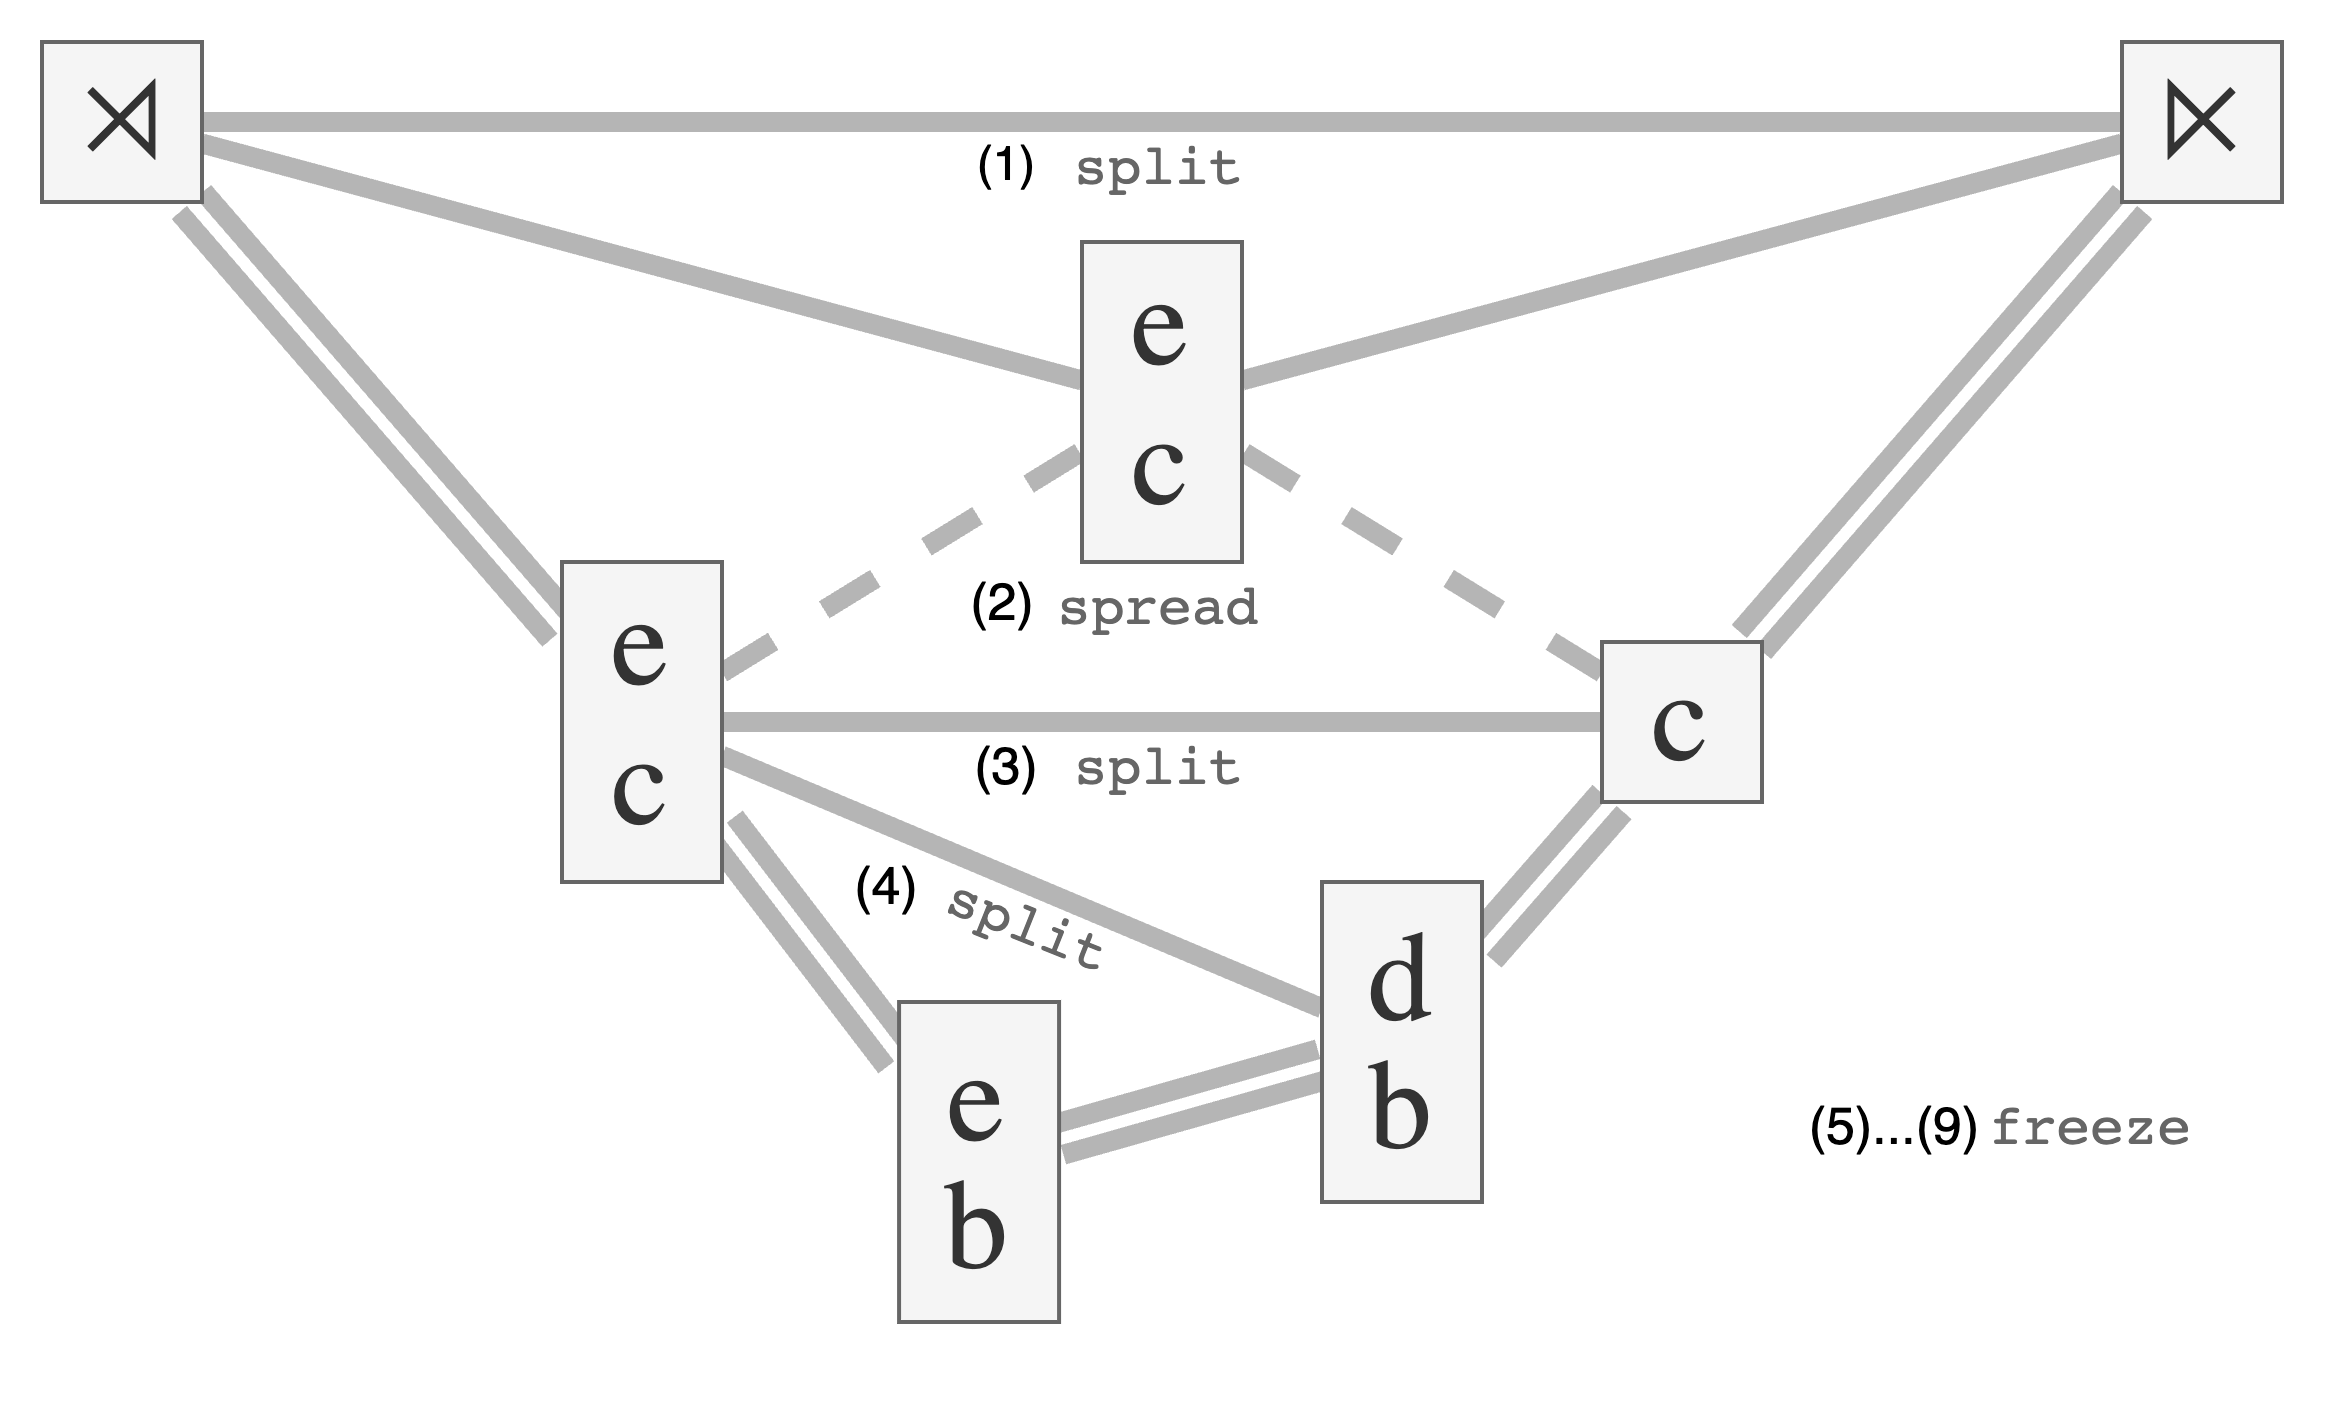
\includegraphics[keepaspectratio,width=\textwidth]{prep/cadenceouterder.png}
    \caption{Outer structure}
    \label{fig:cadenceOuterDer}
  \end{subfigure}
  \begin{subfigure}[t]{.42\textwidth}
    \centering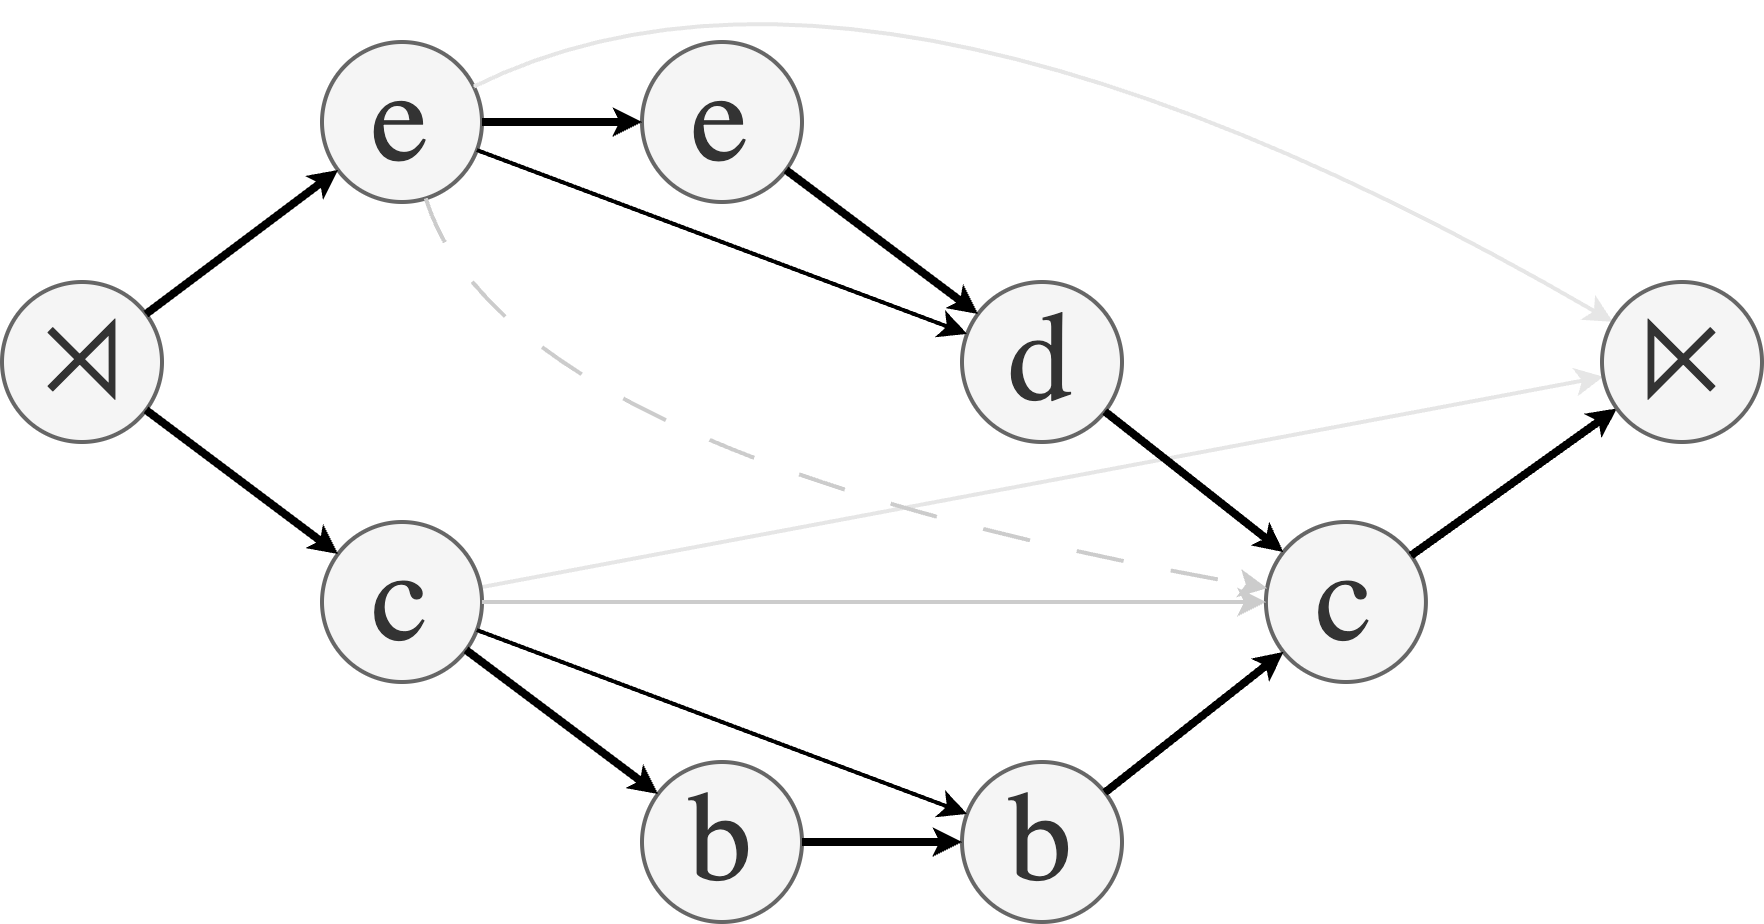
\includegraphics[keepaspectratio,width=\textwidth]{prep/cadenceinnerder.png}
    \caption{Inner structure}
    \label{fig:cadenceInnerDer}
  \end{subfigure}
  \begin{subfigure}[t]{.8\textwidth}
    \centering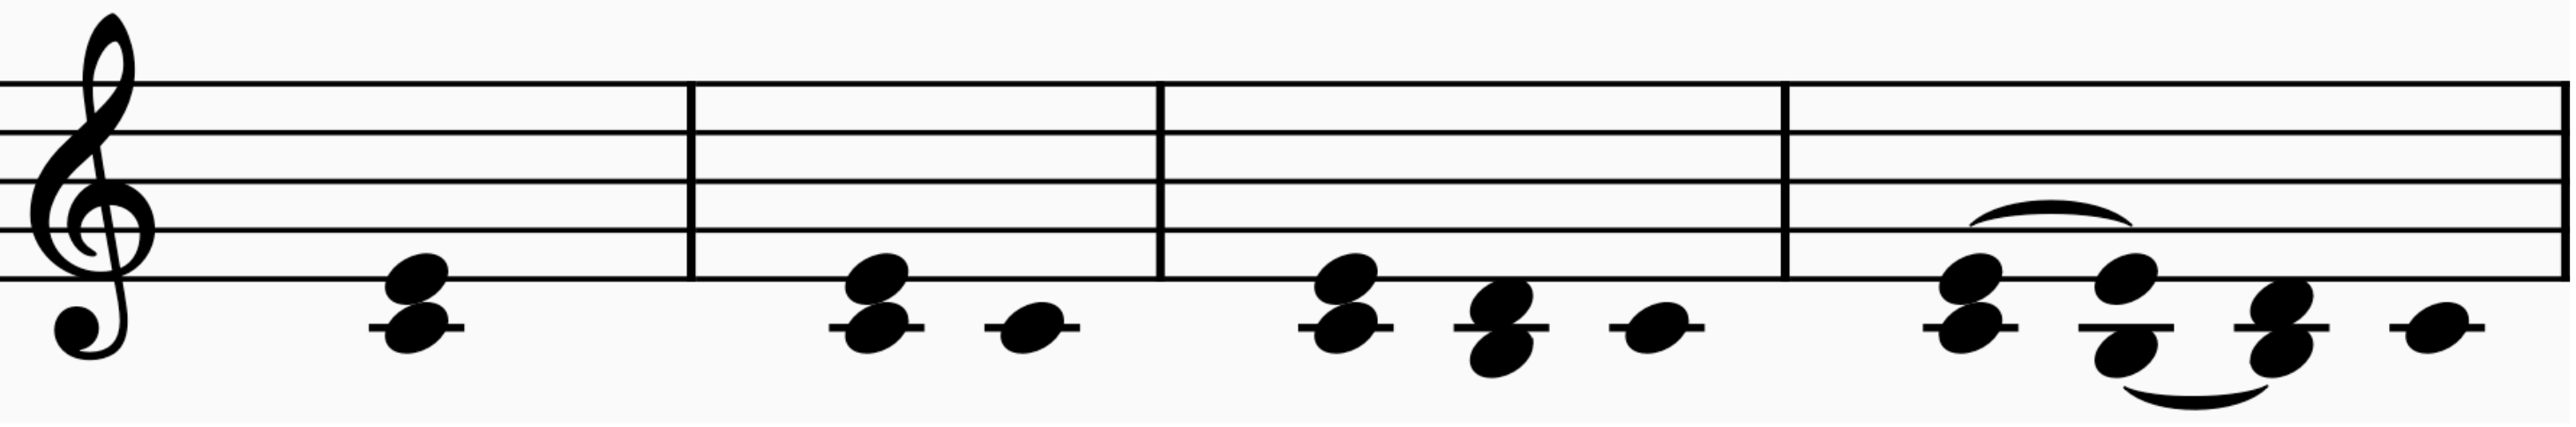
\includegraphics[keepaspectratio,width=\textwidth]{prep/cadencederivation.png}
    \caption{Abstract notation}
    \label{fig:cadenceDerivation}
  \end{subfigure}

  \captionsetup{width=.9\linewidth}
  \caption{An example derivation of the phrase shown in Figure~\ref{fig:cadenceVoices}. }
  \label{fig:innerOuterStructure}
\end{figure}

% subsection Outer Structure (end)
\section{Parsing} % (fold)
\label{sub:protovoiceParsing}

The goal of parsing is to find a \textit{plausible derivation} of the given surface. For a derivation to be \textit{plausible}, the \textit{structure} it presents needs be consistent with a valid musical \textit{interpretation}. Although this is non-trivial, plausibility can be approximately represented by a probability distribution, analogously to probabilistic context free grammars(PCFGs).
\par
% \begin{definition}[Reduction]
%   A \textit{reduction} is defined as as the inverse of a generative process, and is synonymous with a \textit{derivation}. When parsing we \textit{reduce} a piece by applying inverses of the generative operations. The structure midway through a parse of a surface is called a \textit{partial reduction} of that surface.
% \end{definition}
\par
\begin{definition}[Derivation plausibility]
  The plausibility of a derivation is given by the product of the probabilities of each of the production rules used. Given a derivation $D$, its plausibility is defined:
  \begin{equation}
    p(D|S) = \prod_{D_i \in D}  p(D_i|S)
  \end{equation}
\end{definition}


Assuming we can calculate $p(d_i|S)$, we can find the most plausible derivation by taking the maximum likelihood estimate (MLE) of the distribution
\begin{equation}
  \hat D = \argmax_{D}  p(D|S)
  \label{eq:mapApproach}
\end{equation}

This presents \textbf{two key problems} to be solved:

\begin{itemize}
  \item \textbf{Calculating} $p(d_i|\text{surface})$. Production probabilities can be viewed as parameters of the model; a common approach with PCFGs is to learn these parameters using machine learning. However, as the protovoice model is not context-free and the volume of data required is not available an alternative method must be found.
  \item \textbf{Combinatorial explosion}: Even if we could calculate $p(D|S)$ analytically, we would be prohibited by the large branching factor; a single piece can have upwards of $9^{9^{9^{{\iddots}^{9^{9}}}}}$ possible derivations\footnote{I need a better way to represent the scale here. Perhaps I'll try to actually estimate a number}.
\end{itemize}

\section{Heuristic Search Algorithms}

Heuristic search algorithms are introduced in 1B \textit{Artificial Intelligence}, so I will therefore assume the reader has knowledge of the heuristic search paradigm.

The naive way to solve the above parsing problem is to use an \textit{exhaustive search} strategy. This would theoretically allow us to find the most plausible derivation, but is computationally infeasible.

\textbf{Best-first search} is a heuristic search algorithm that selects the most \textit{promising} node to expand based on a heuristic evaluation function. 
In general, the heuristic function $h(n)$ depends on  the description of $n$, the description of the goal, information gathered by the search up to that point, and most importantly domain specific knowledge\cite{pearlHeuristicsIntelligentSearch1984}.

\textbf{Beam search} is an optimisation of best-first search that serves to reduce its memory requirements by only storing a limited number of best states as candidates to expand, dependent on the \textit{beam width}. Beam search is greedy algorithm, so it does not necessarily produce the optimal solution, but trades optimality for improved complexity.

% \textbf{Stochastic beam search} is a further optimisation of beam search 
%
% of best-first search that serves to reduce its memory requirements by only storing a limited number of best states as candidates to expand, dependent on the \textit{beam width}. 

% Heuristic search algorithms are a subset of search algorithms used to find a sequence of actions from an initial state that results in a goal state.  The problem is defined as follows:
% \begin{itemize}
%   \item We have an \textit{initial state} $s_0$ where $s_0 \in S$, the set of possible states
%   \item We have set of \textit{actions} $A$, modelled by the function $action: A\times S \to S$
%   \item We have \textit{goal test}, modelled by the function $goal: S \to \{true, false\}$
%   \item There is a \textit{cost} associated with every path, modelled by $cost: A \times S \to \mathbb{R}$
%   \item Finally, we have a function \textit{expand} is a \textit{cost} associated with every path, modelled by $cost: A \times S \to \mathbb{R}$
%   \item We wish to find the minimum cost path from the initial state $s_0$ to a goal state. 
%   % \item We have an initial state $s_o \in S$, which is the empty reduction, corresponding to the unreduced surface of the piece. The score is represented as a sequence of slices grouping notes that sound simultaneously. We are also given the segmentation of the original chord labels that we wish to retrieve.
%   % \item We have a set of actions, $A$ modelled by a function $action: A \times S \to S$. These actions correspond to a single reduction step.
%   %   \begin{itemize}
%   %     \item The reduction steps are the inverses of the operations defined by the generative proto-voice model.
%   %   \end{itemize}
%   % \item Finally we have a goal test, $goal: S \to \{true,false\}$ which is true iff the partial reduction $s$ has exactly one slice per segment of the input.
%   %   \begin {itemize}
%   % \item This means the partial reduction $s$ contains a sequence of slices which start and end positions corresponding to the segmentation of the piece.
%   %   \end {itemize}
%   % \item At the first stage, this will be implemented using a random graph search algorithm, picking each action randomly, according to precomputed distributions.
%   % \item The state space $S$ is the set of all possible partial reductions of a piece along with each reduction step that has been done so far. 
%   % \item We have an initial state $s_o \in S$, which is the empty reduction, corresponding to the unreduced surface of the piece. The score is represented as a sequence of slices grouping notes that sound simultaneously. We are also given the segmentation of the original chord labels that we wish to retrieve.
%   % \item We have a set of actions, $A$ modelled by a function $action: A \times S \to S$. These actions correspond to a single reduction step.
%   %   \begin{itemize}
%   %     \item The reduction steps are the inverses of the operations defined by the generative proto-voice model.
%   %   \end{itemize}
%   % \item Finally we have a goal test, $goal: S \to \{true,false\}$ which is true iff the partial reduction $s$ has exactly one slice per segment of the input.
%   %   \begin {itemize}
%   % \item This means the partial reduction $s$ contains a sequence of slices which start and end positions corresponding to the segmentation of the piece.
%   %   \end {itemize}
%   % \item At the first stage, this will be implemented using a random graph search algorithm, picking each action randomly, according to precomputed distributions.
% \end{itemize}
%
% subsection protovoiceParsing (end)
\section{Inferring Labels}

The task of inferring harmony (ACE) poses \textbf{three main challenges}: 
\begin{itemize}
  \item \textbf{Segmentation}: Segmentation is splitting of the score into segments which each have an individual label. For example, Figure~\ref{fig:pvHarmony} shows each segment separated by a dashed grey line. As these segments are typically not given a priori, both the segmentation and harmony needs to be inferred. Performing the joint task of segmentation and labelling is beyond the scope of this project, however, so we will assume that the segmentation is given.
  \item \textbf{Ambiguity}: The notes in a given segment may not be enough to determine the chord label. For example, the slice containing notes D and B in Figure~\ref{fig:pvHarmony} could be a realisation of a Bm triad, but the context of the neighbouring slices as well as the functional dependencies of the notes makes it clear that the label should be a G. Furthermore, ambiguity is often used with much license to create artistic interest.
  \item \textbf{Non chord-tones}: The slices in a given segment will typically consist of combination of \textit{chord-tones} and \textit{non chord-tones}. The chord tones directly define the harmony, so to perform ACE, an algorithm will need to distinguish between the two. Previous approaches have involved modelling generation as a noisy process, such that the non chord-tones are considered as noise\cite{temperleyAlgorithmHarmonicAnalysis1997}. The protovoice model allows us \textit{explicitly} explain away non chord-tones. 
    In Figure~\ref{fig:pvHarmonyUnreducedOuter}, the non chord-tone is denoted in red. 
    By applying a reduction that removes the neighbour note, E, we result in a single slice in that segment which only contains chord-tones(Figure~\ref{fig:pvHarmonyReducedOuter}), thus describing the chord label more clearly, shown in Figure~\ref{fig:pvHarmonyReducedInner}.
\end{itemize}

\begin{figure}[h]
  \centering
  \begin{subfigure}[t]{.44\textwidth}
    \centering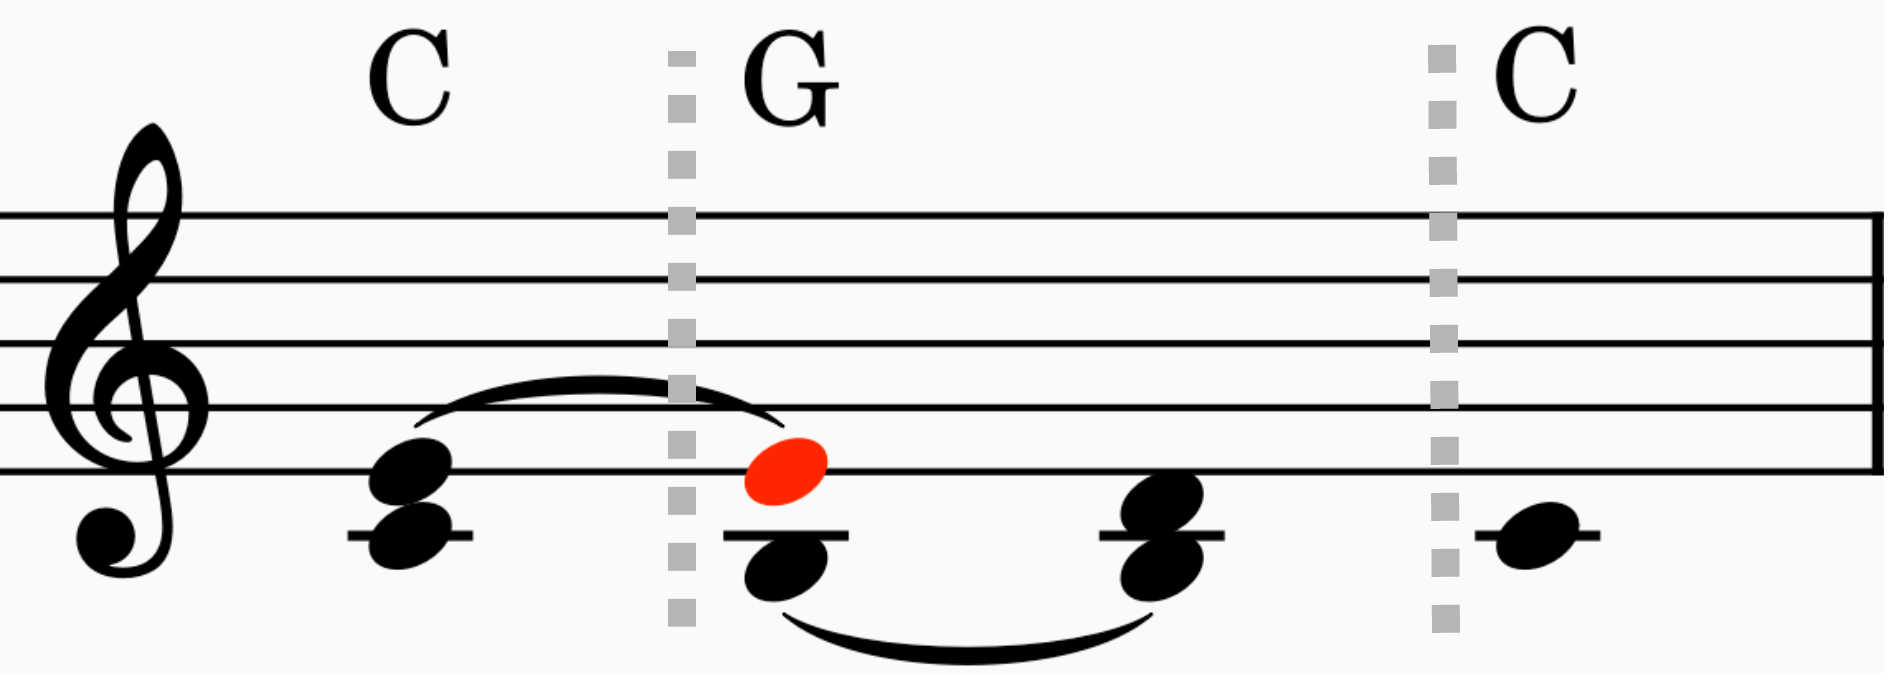
\includegraphics[keepaspectratio,width=\textwidth]{prep/harm/unreducedScore.png}
    \caption{}
    \label{fig:pvHarmonyUnreducedInner}
  \end{subfigure}
  \begin{subfigure}[t]{.44\textwidth}
    \centering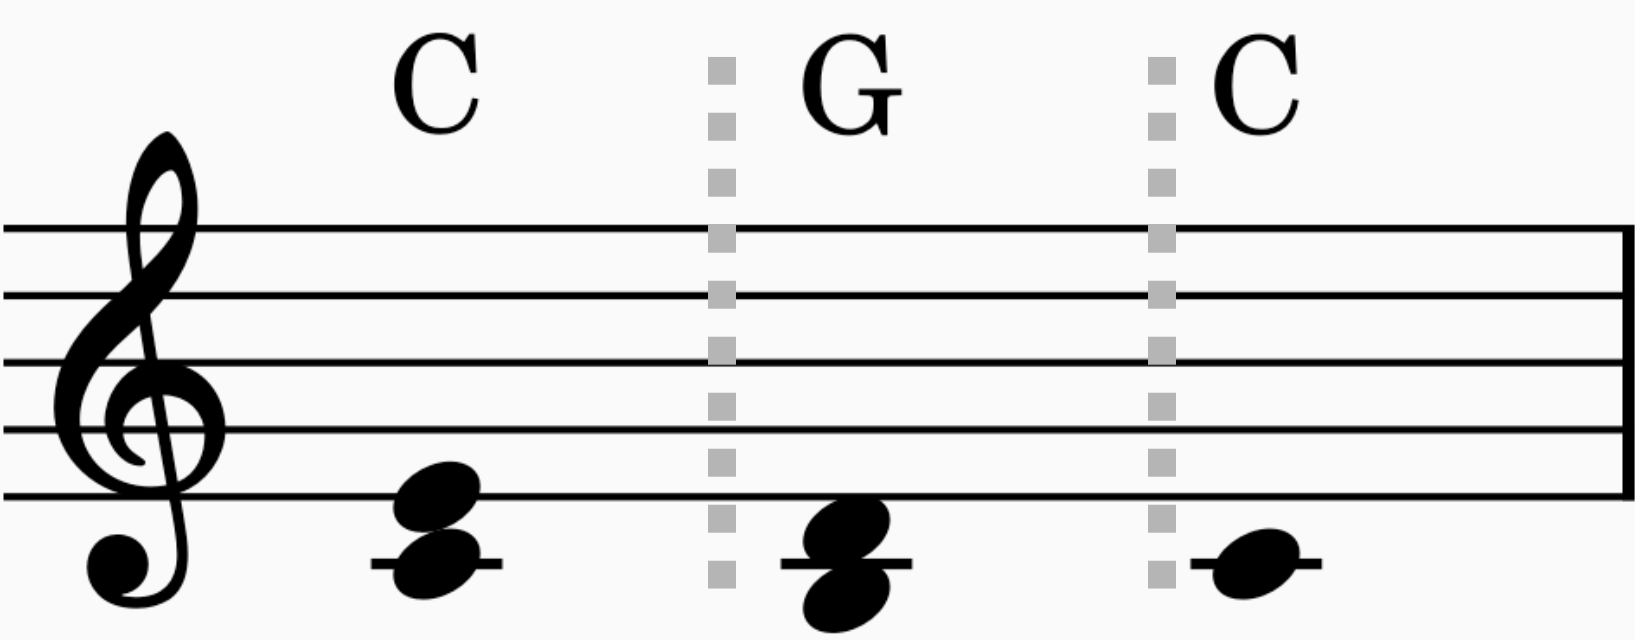
\includegraphics[keepaspectratio,width=0.85\textwidth]{prep/harm/reducedScore.png}
    \caption{}
    \label{fig:pvHarmonyReducedInner}
  \end{subfigure}

  \begin{subfigure}[t]{.496\textwidth}
    \centering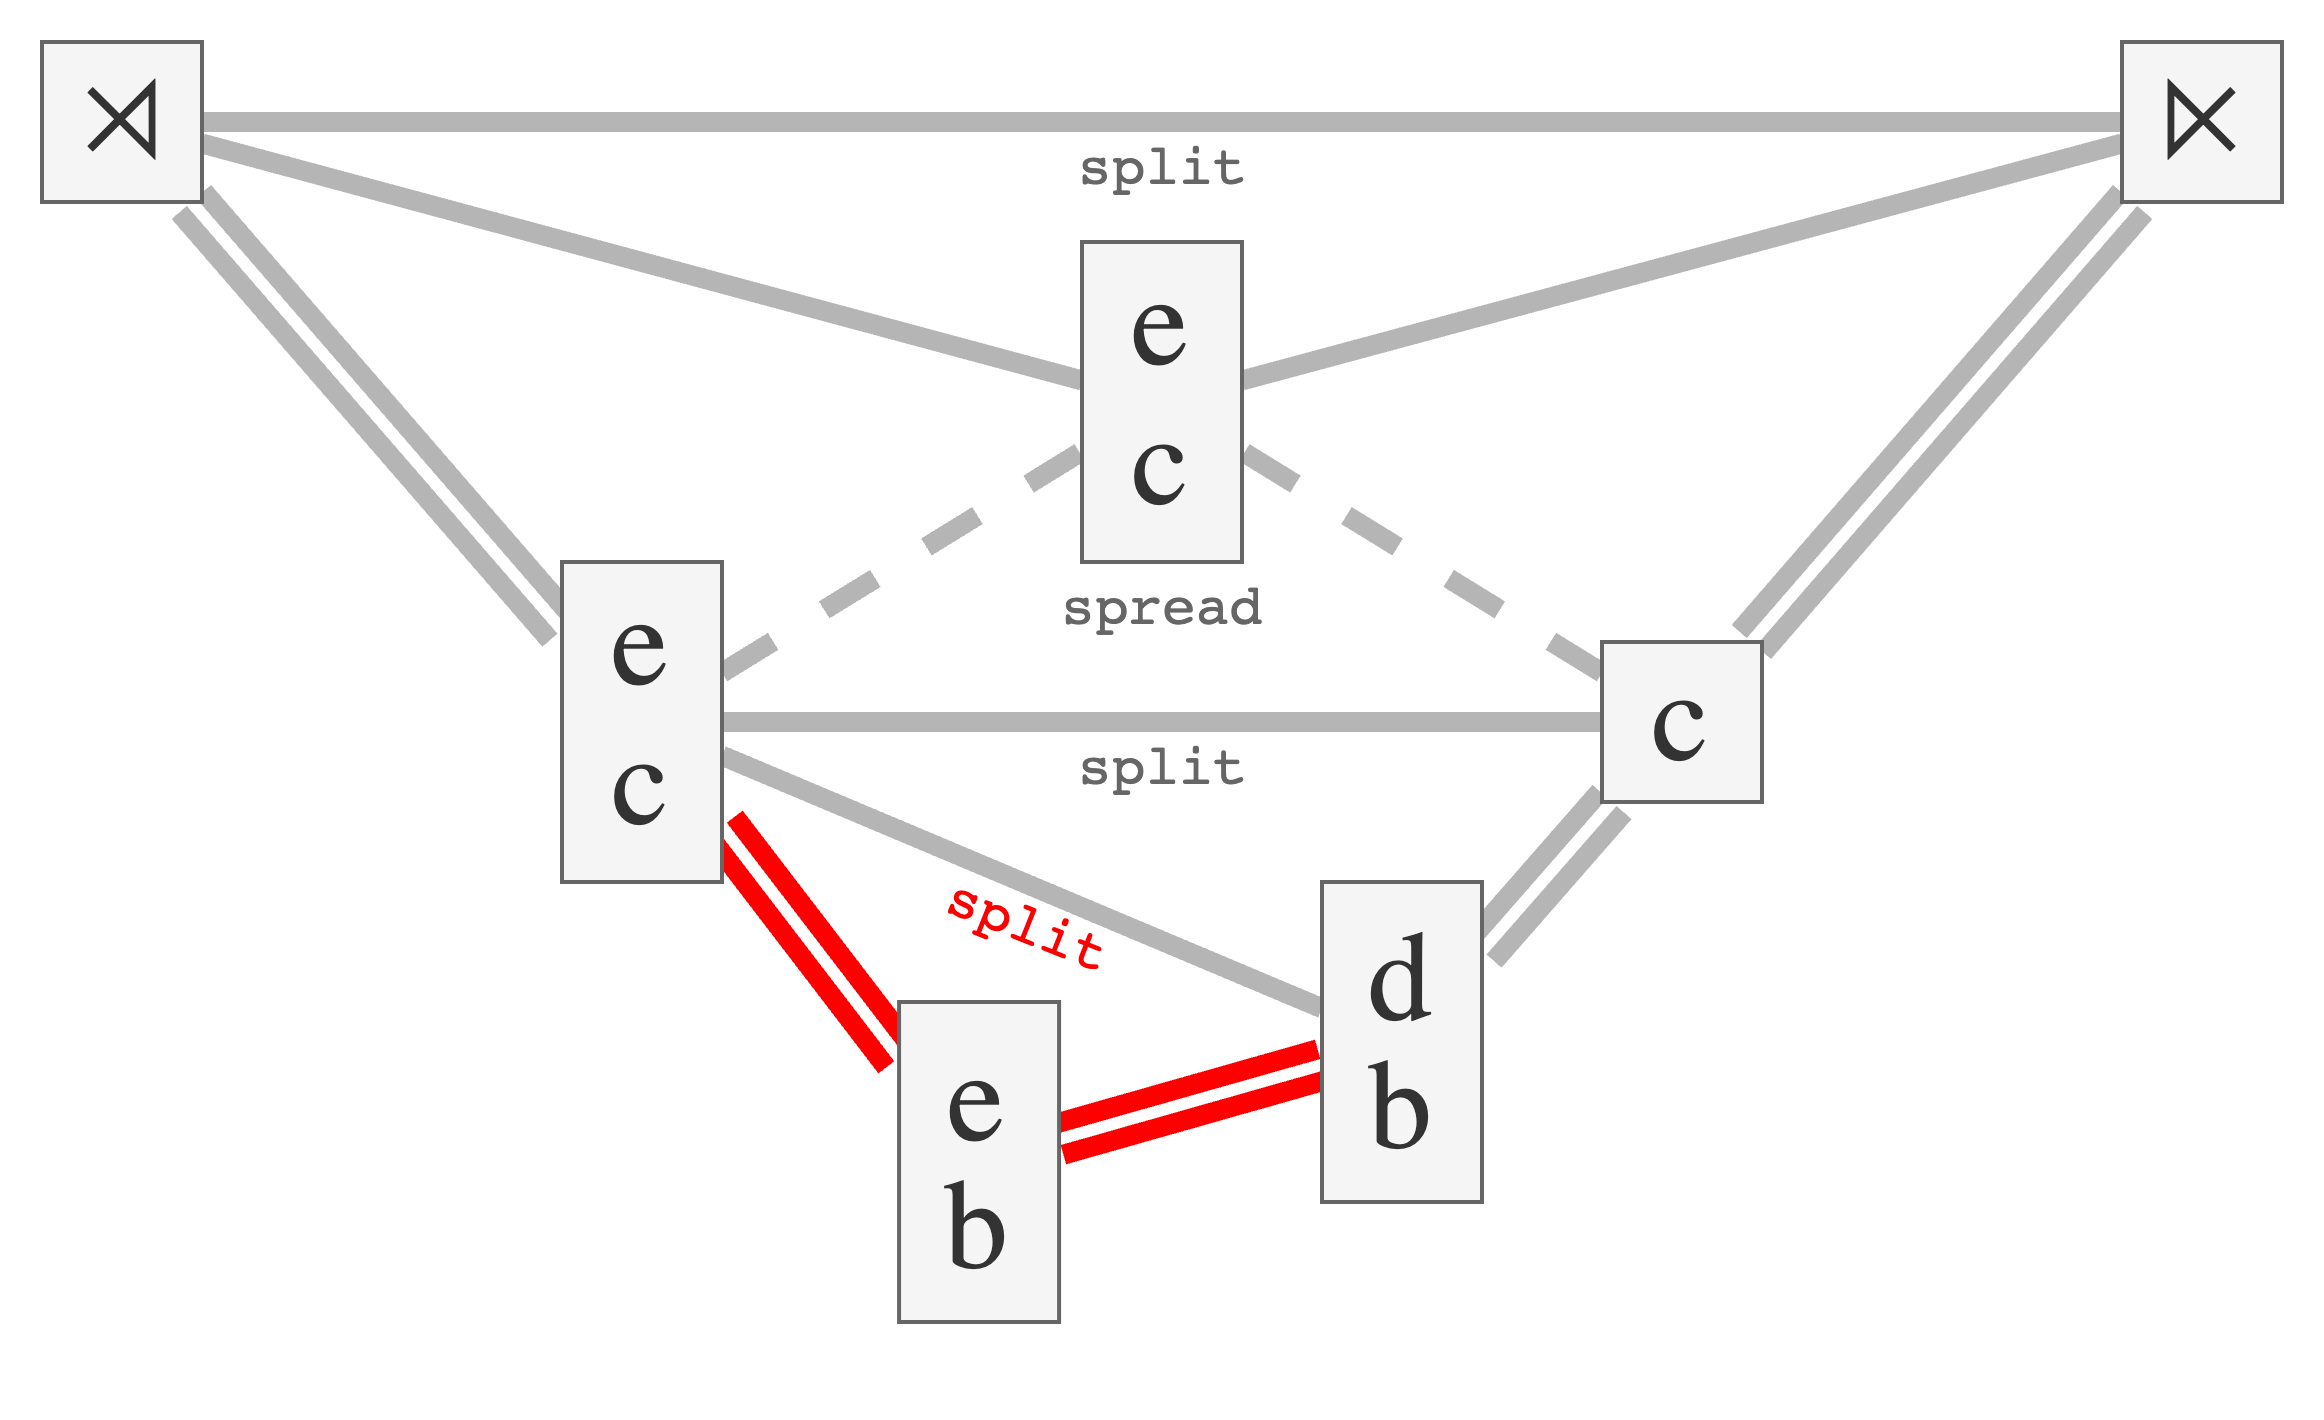
\includegraphics[keepaspectratio,width=\textwidth]{prep/harm/unreducedOuter.png}
    \caption{}
    \label{fig:pvHarmonyUnreducedOuter}
  \end{subfigure}
  \begin{subfigure}[t]{.496\textwidth}
    \centering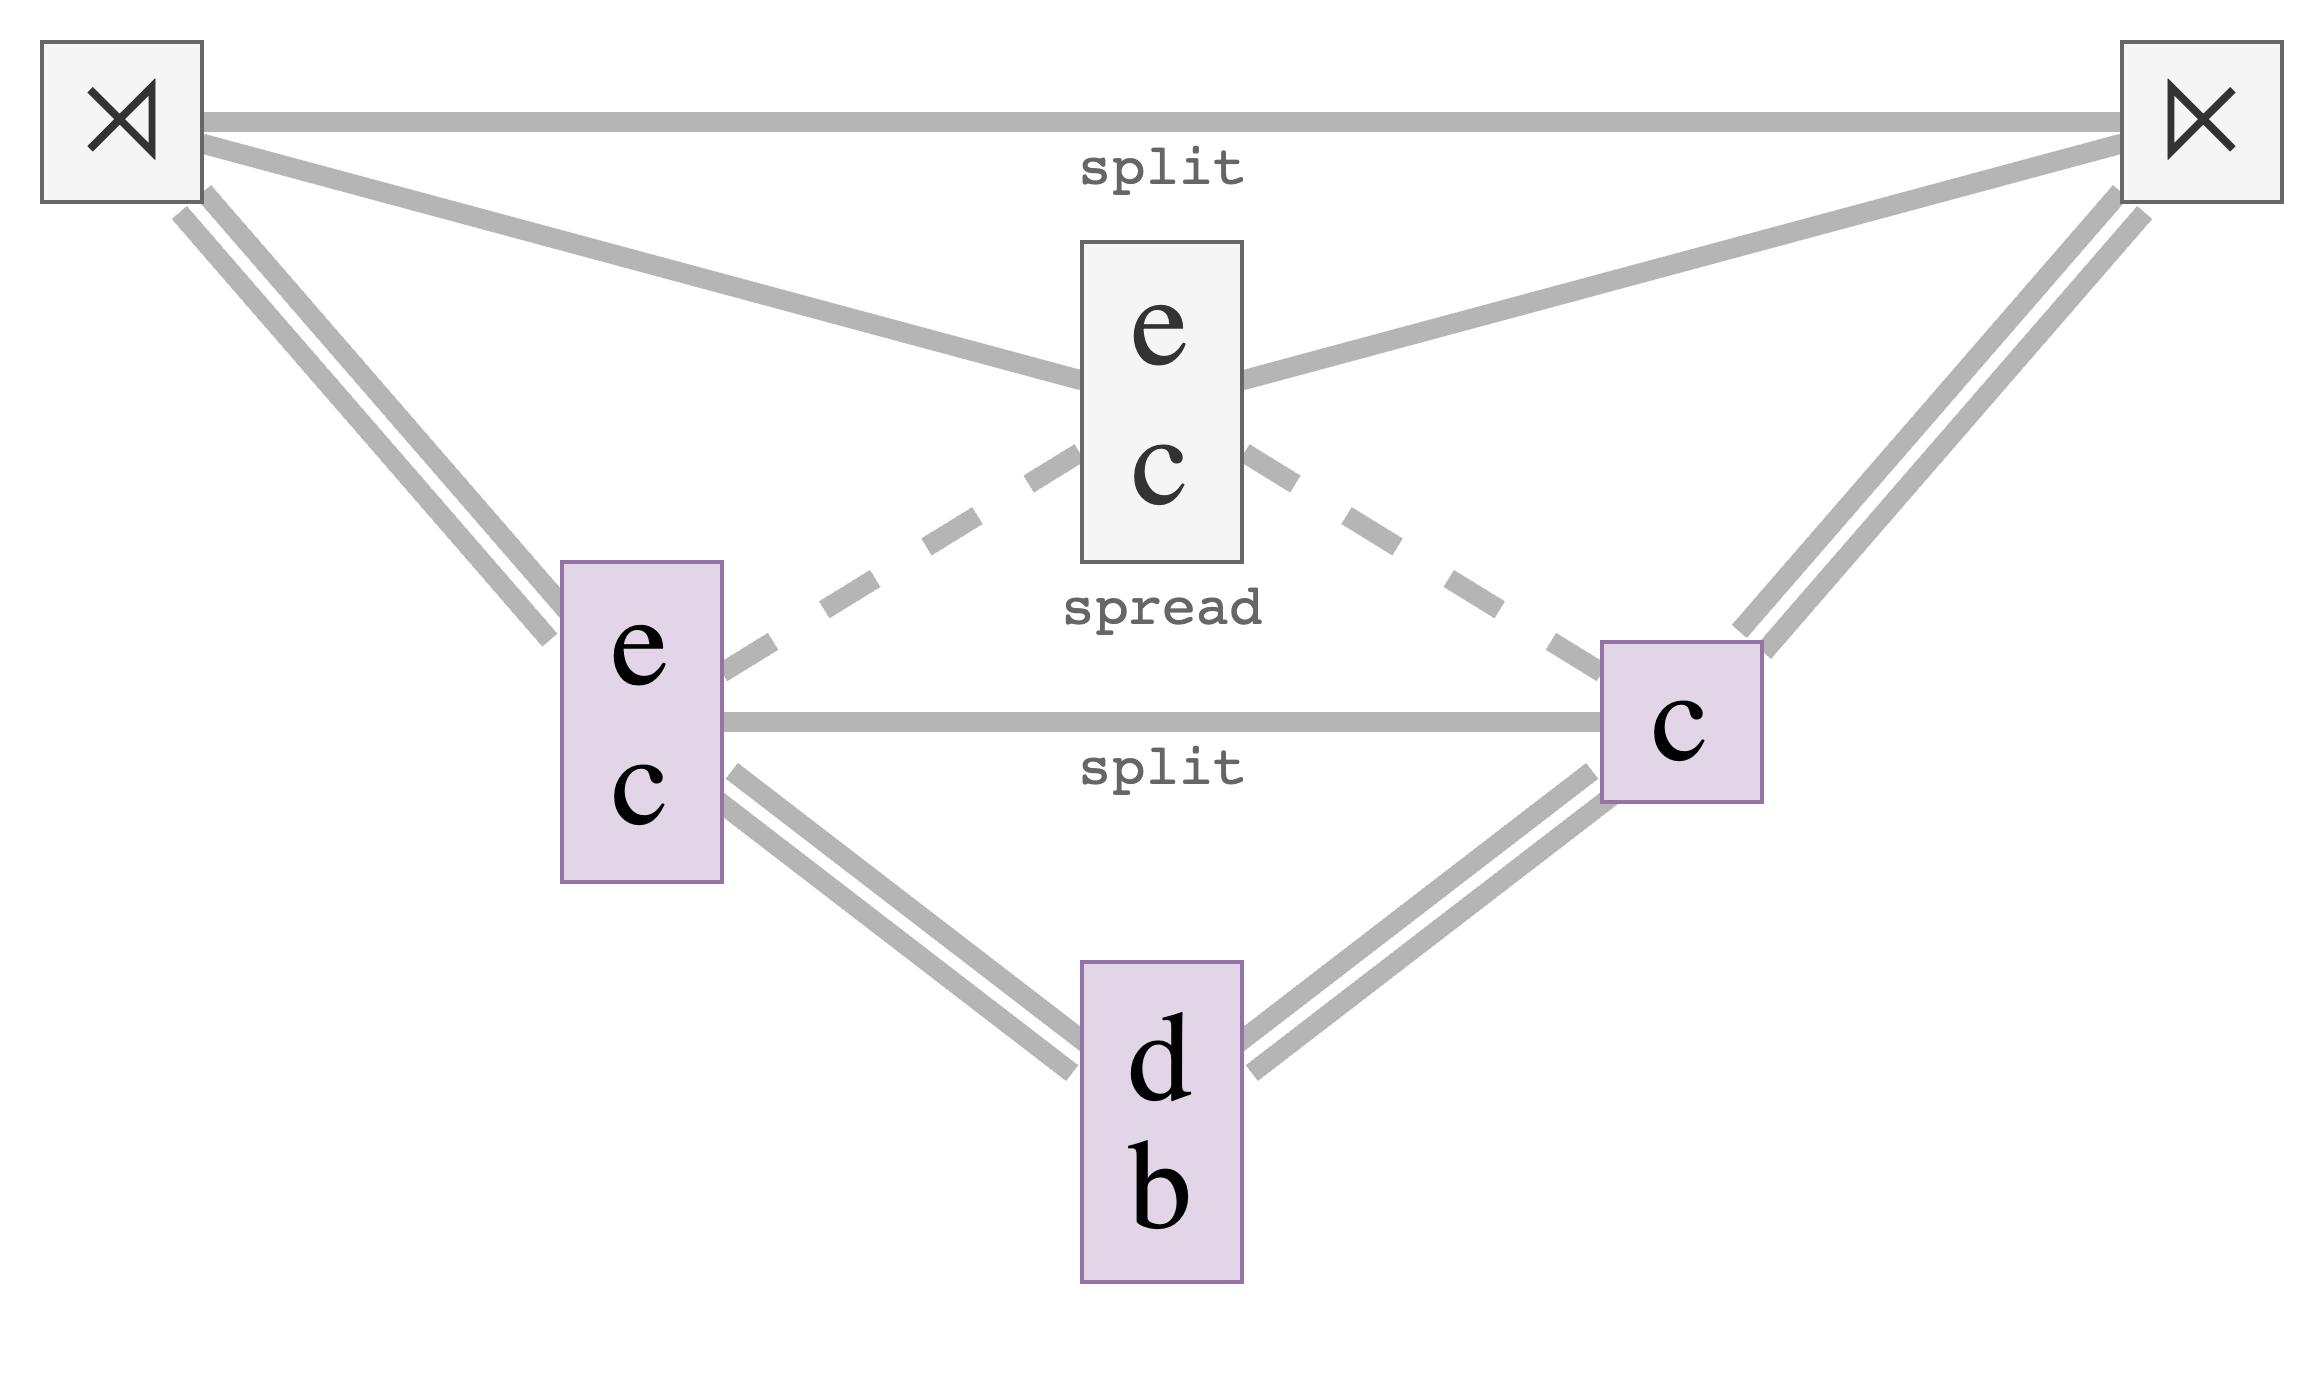
\includegraphics[keepaspectratio,width=\textwidth]{prep/harm/reducedOuter.png}
    \caption{}
    \label{fig:pvHarmonyReducedOuter}
  \end{subfigure}

  \captionsetup{width=.9\linewidth}
  \caption{Applying a reduction to aid harmonic inference}
  \label{fig:pvHarmony}
\end{figure}


% We can \textit{factorize} a probabity distribution into a \textit{prior} and a \textit{likelihood}. By choosing priors that are conjugate to the likelihood, we get a posterior distribution that is 
%
% Provide an explanation of all the concepts I learned and used in this project. 
% Techniques such as marginalisation, joint distributions, bayes rule etc. 
%
% Dirchelet distributions
%
% Beta distribution  
%
% Multinomiall distribution 
%
% Normal Distribution 
%
% \par 
% Inference as model $\to$ data $\to$ prob distribution $\to$ chord guess

\footnote{I'm considering adding a small section describing some relevant distributions. Dirchelet, Beta, Multinomial, categorical? It took a while for me to get my head around the fact that we used probability distributions of parameters of other probability distributions, e.g. sampling from Dirichlet for parameters of a multinomial or categorical.}

\section{Starting Point}

\subsection{Relevant courses and experience}

\paragraph{Haskell}{I was introduced to Haskell during an internship during the summer before starting this project (July to August 2022). As a result, I had 2 months of experience with the language beforehand. I chose to use Haskell in order to further familiarise myself with the language, and because of its amenability to parsing algorithms. Furthermore, the functional paradigm and rich type system lends itself to modular software development.}

\paragraph{Python}{I have experience coding in Python from personal projects as well as the 1A \textit{Scientific Computing Practical Course}. This was chosen to made use of powerful existing libraries for handling large datasets and running experiments. }

\paragraph{IB}{ Two modules from 1B provide a foundation for this project. \textit{Formal Models of Language} introduces the ideas and terminology used in the protovoice model, and \textit{Artificial Intelligence} provides a background for classical search algorithms as well as some of the probabilistic frameworks used in the project.}

\subsection{Existing codebase}
This project was built on a fork of the pre-existing \textit{protovoices-haskell} GitHub repository. This repository contains custom data structures and types, allowing interoperability with other projects making use of the same model. I also make use of learned parameters from the implementation of the paper \textit{Bayesian Model of Extended Chord Profiles}\cite{finkensiepChordTypesOrnamentation2023}, as learning these parameters would be beyond the scope of this project. 

\section{Requirements Analysis}
\subsubsection{Success Criteria}
The Success Criteria are given in the \nameref{chap:proposal}. During the preparation phase, I refined the Success Criteria by gaining clarity from the literature related to the project. 

This project will be deemed a success given it achieves:
\begin{itemize}
  \item 
\end{itemize}

\subsubsection{Risk Assessment}

Table~\ref{tab:deliverables} shows a list of project deliverables with associated priorities and risk, denoted qualitatively. There is a high general risk in this project due to the fact that the protovoice model is a result of an unpublished thesis, and thus may have flaws that have not been discovered. The highest risk task is designing and implementing the protovoice parser. The heuristic design task is expansive, requiring creativity, research and iterative development, hence the risk is high. The baseline inference deliverable comprises a standard method for ACE, so there is minimal risk.

\begin{table}[h]
  \caption{Project Deliverables}
  \vspace{\baselineskip}
  \label{tab:deliverables}
  \centering
  \begin{tabularx}{0.9\textwidth}{cXcc}
    {\large \textbf{ID}} & \large \textbf{Deliverable} & \large \textbf{Priority} & \large \textbf{Risk} \\
    \toprule
    \texttt{core1} & Harmony Model & High & Low \\
    \texttt{core2} & End to End Pipeline  & High & Medium \\
    \texttt{core3} & Protovoice Parser & High & High \\
    \texttt{base1} & Baseline Reduction & High & Low \\
    \texttt{base2} & Random Search & High & Low \\
    \texttt{ext1} & Heuristic Design & Medium & High \\
    \texttt{ext2} & Greedy Search & Medium & Medium \\
    \texttt{ext3} & Beam Search & Low & Very High \\
    \texttt{ext4} & Dual Beam Search & Low & Very High \\
  \end{tabularx}
\end{table}


\section{Software Engineering Techniques}

\subsection{Development model}
Based on the risk analysis (Table~\ref{tab:deliverables}), I created a plan of which modules to implement in which order, and a list of milestones on a 2 week basis. I used Notion to maintain a list of core tasks and corresponding subtasks with associated priorities, which I used when deciding what to work on. My development strategy drew from the Agile methodology, working on tasks in two-week long sprints, with regular re-evaluations of the plan informed by experimental data and testing.

I made use of GitHub's continuous integration features to run a test suite on the repository after every commit.  

\subsection{Languages, libraries and tools}

\begin{table}[h]
  \caption{Languages, libraries and tools}
  \label{tab:languages}
  \centering
  \footnotesize
  \renewcommand{\arraystretch}{1.3}
  \begin{tabularx}{\textwidth}{p{4em}X X p{4em}}
    {\normalsize \textbf{Tool}} & {\normalsize \textbf{Purpose}} & {\normalsize\textbf{Justification}} & {\normalsize \textbf{License}} \\
    \toprule
    \textit{Languages} &&&\\
    Haskell & Main language used for the core, baseline and extension implementations 
            & Protovoice model implementation is in Haskell. Functional and amenable to parser development.
            & GHCL \\

    Python & Secondary language for experiments and analysis 
           & Powerful library ecosystem for running experiments and creating plots 
           & PSFL \\

    \midrule
    \textit{Libraries} &&&\\
    Musicology & Haskell Library with data-types for pitches 
                       & Contains a robust implementation of spelled pitch classes, which would be tedious to reimplement.
                       & BSD-3.0 \\
    Timeit & Lighweight wrapper to show the used CPU time of a monadic computation
           & This is used to time the runtime of the algorithms as part of analysis
           & BSD-3.0 \\
    Dimcat & Python library: DIgital Musicology Corpus Analysis Toolkit 
           & This library was written to work with the datasets used in this project 
           & GPL-3.0 \\
    Numpy & Python library used for preprocessing and analysis
          & Powerful standard library that is used in conjunction with Seaborn to run analysis and visualise data
          & BSD-3.0 \\
    Pandas & Python library for preprocessing and analysis
           & This is a standard library for data manipulation and processing
           & BSD-3.0 \\
    Seaborn & Python data visualisation library used for analysis
            & Creates high quality graphs and charts
            & BSD-3.0 \\
    \midrule

    \textit{Tools} &&&\\
    Docker & Containerised software service used to run repeatable experiments 
           & The use of many libraries creates a web of dependencies to be resolved. Ensures the code will last and can be executed on different devices 
           & Free/Paid \\
    Git & Version Control, Continuous Integration 
        & Provides natural backups and allows for reverts to previous commits if necessary
        & GPL-3.0 \\
    GitHub & Hosting source code
           & Free, reliable hosting
           & GPL-3.0 \\
    GHC & Compiling and profiling.
        & This is the standard Haskell compiler. 
        & BSD-3.0 \\
    Stack & Haskell building and testing  
        & Creates reliable builds, and includes a powerful testing framework.
        & BSD-3.0 \\
    Undotree & Vim Plugin: stores all past actions as a tree 
        & Solves the problem of linear undo history being lost. Protects code between commits. 
        & BSD-3.0 \\
    MuseScore & Music notation software 
                & The raw inputs are in the MusicXML format, which is used by MuseScore 3
                & GPL-3.0 \\
    PAT & Protovoice Annotation Tool, Used to view protovoice derivations on a web browser 
          & The protovoice derivations are huge and very complex, so it's vital to have a viewing tool for use in analysis and iterative development
        & GPL-3.0 \\
  \end{tabularx}
\end{table}

Table~\ref{tab:languages} shows a justified list of the key languages, libraries and tools used in the project.

\FloatBarrier
\subsection{Licensing}

As shown in Table~\ref{tab:languages}, I determined and read up on all of the licensing agreements for the tools used in the project. For the most part, these are all permissive licenses, guaranteeing freedom to use, modify and redistribute as well as permitting proprietary derivative works. 

\subsection{Datasets}


\subsection{Hardware, version control and backup}
The code was developed using Vim for Haskell and Visual Studio Code for Python notebook development, on my personal laptop (16' MacBook Pro 2022, M1 Max, 32GB). 
Experiments were run first locally, then on HPC provided by the EPFL Digital Cognitive Musicology Lab (Dell PowerEdge R740XD Server, 2x Xeon Gold 625R, 768GB), using Jupyter notebooks to conduct the evaluation. I used GitHub for all my notes, development and dissertation writing. Finally, this dissertation was written in Vim with VimTeX.

%%%%%%%%%%%%%%%%%%%%%%%%%%%%%%%%%%%%%%%%%%%%%%%%%%%%%%%%%%%%%%%%%%%%%
% Implementation
%%%%%%%%%%%%%%%%%%%%%%%%%%%%%%%%%%%%%%%%%%%%%%%%%%%%%%%%%%%%%%%%%%%%%

\chapter{Implementation}

\section{ProtoVoice Harmony Model}
\subsection{Overview}

We present a \textbf{novel} inference system, the \textbf{ProtoVoice Harmony Model} that approximates $\argmax_L P(L|S)$ to infer harmony from free polyphony.


\begin{figure}[h]
  \centering
  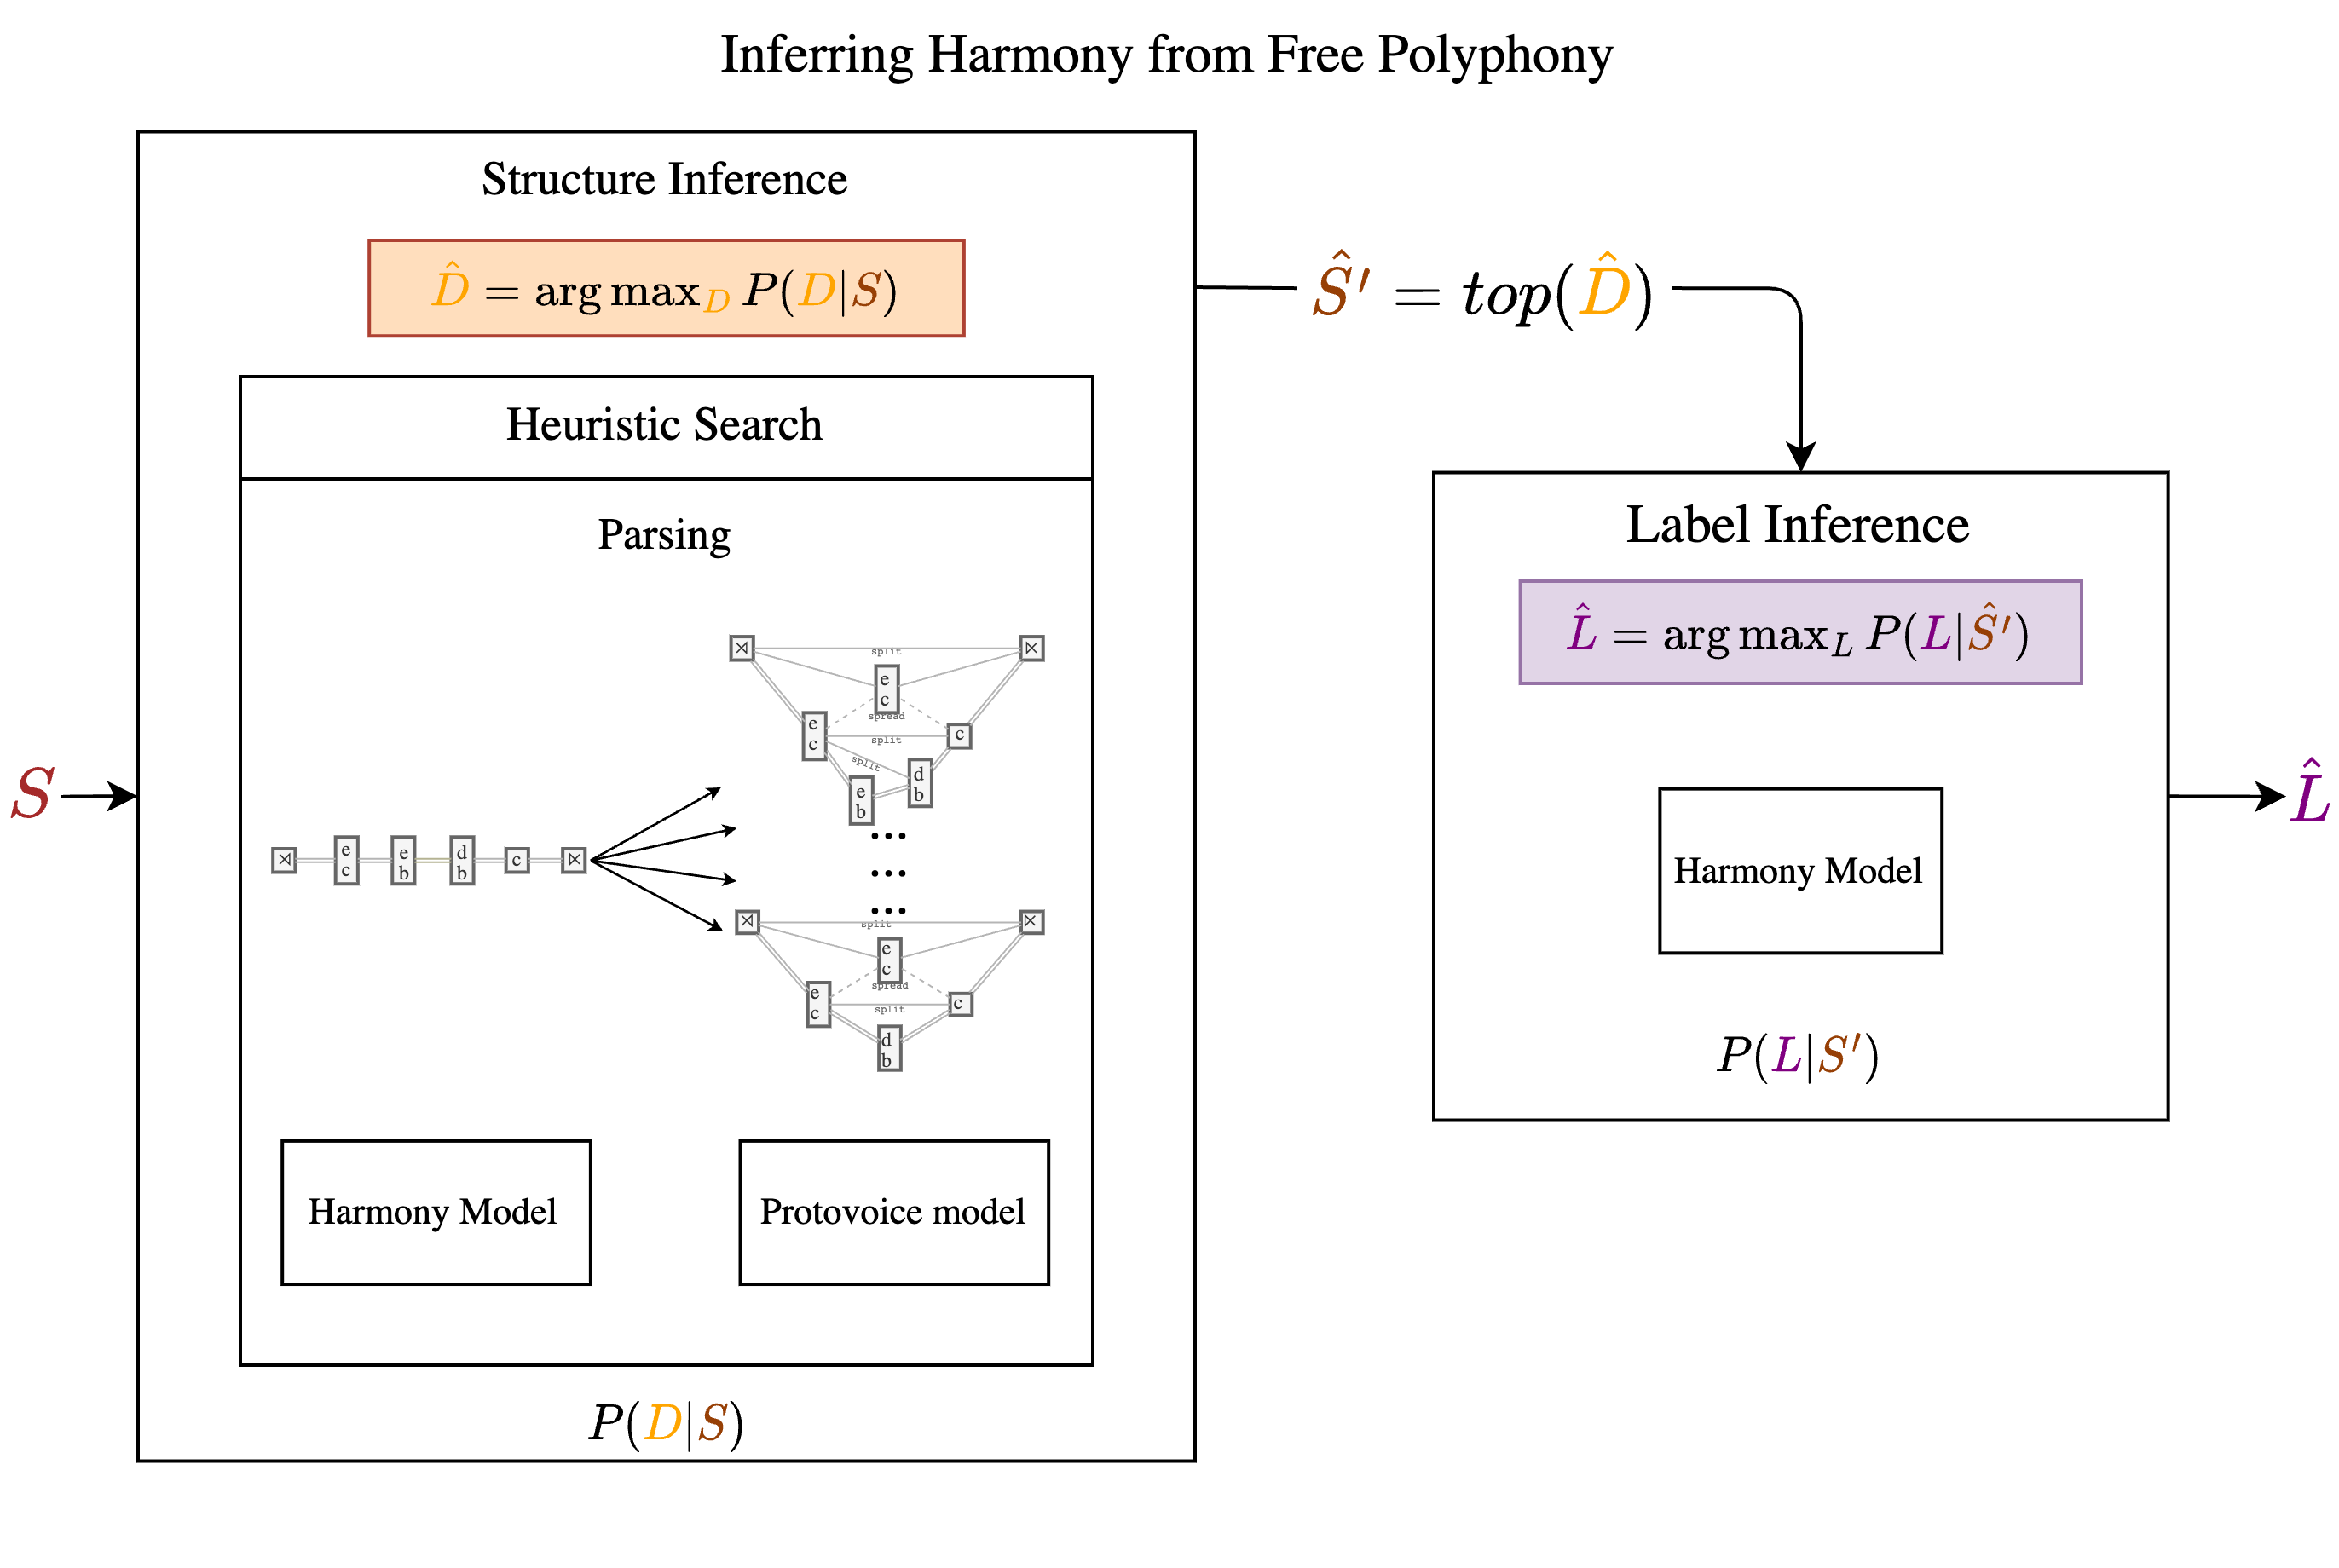
\includegraphics[width=\textwidth]{intro/inferenceOverview}
  \caption{Overview of the inference process.}
  \label{fig:inferenceOverview}
\end{figure}

% \begin{equation}
%   P(S|L) = \sum\limits_{D,S'} P(S|D)~P(D|S')~P(S'|L)
%   \label{eq:inferencePVEQ}
% \end{equation}

The PVHM is described by the following equation: 
\begin{equation}
  \label{eq:pvhmSuccinct}
  \begin{gathered}
  \hat{L} = \argmax_L \Left( P(S|L, \mathcal{R}(S)) \cdot P(L) \Right)\\
  \text{where $\mathcal{R}: \mathbf{S} \to \mathbf{S'}$ is given by:} \\
  \mathcal{R} (S) = top \left(\argmax_D P(D|S) \right) \\
  \end{gathered}
\end{equation}

The core of this model is that we find the most likely reduction $\mathcal{R}(S)$ of the surface $S$ by inferring the most likely protovoice structure $\hat{D}$, using $top:\mathbf{D} \to \mathbf{S'}$. Given the reduced surface $\mathcal{R}(S)$ we finally solve $\hat{L} = \argmax_L P(L|S, \mathcal{R}(S)) \cdot P(L)$, finding the most likely sequence of chord labels $\hat{L}$ given the reduced surface $\mathcal{R}(S)$

\subsubsection{Development plan}
This system is modular by design, leading to a natural progression of complexity throughout the implementation; the baseline models provide a subset of the functionality required for the full system. For example, the harmony model is a prerequisite for the first baseline, but is also used in all subsequent models. \footnote{This could be complemented by a diagram showing the progression}

\begin{itemize}
  \item The Baseline Reduction computes a simplified $\mathcal{R}(S)$ using random sampling. 
  \item The Random Search uses $\mathcal{R}(S) = top (D_0)$, where $D_0$ is the derivation found by randomly choosing each parse operation. 
  \item The first extension involves developing an informed heuristic $\mathcal{H}_0$
  \item The Greedy Search uses heuristic $\mathcal{H}_0$ to approximate $\argmax_D P(D|S)$.
  \item The Beam Search uses $\mathcal{H}_0$ to implement a search parameterised by the beam width $\beta$
  \item The Dual Beam Search implements a custom search algorithm using $\mathcal{H}_0$, parameterised by $\alpha$ and $\beta$, which control operation dependent beam widths.  
\end{itemize}

% \begin{equation}
%   P(S|L) = \sum\limits_{D,S'} P(S|D)~P(D|S')~P(S'|L)
%   \label{eq:inferencePVEQ}
% \end{equation}
\section{Repository Overview:}

\subsubsection{Repository Justification}

The repository has been split into four main folders, with the addition of \texttt{Main.hs} which serves as an interface between the python experiment code and the algorithms developed in Haskell. 
\begin{itemize}
  \item Firstly, the \texttt{src/Core/} folder contains all the core code, including the implementation of the parsing  and inference functions using the probabilistic model of harmony, as well as some helper code for file handling. 
  \item The \texttt{experiments/} folder contains all the python code that is used for this project. The experiments consist of three stages, as described by the three main files: \texttt{preprocess.py}, \texttt{experiments.py} and \texttt{analysis.py}. Splitting these stages up prevents wasteful computation, as all the pre-processing can be done just once, while experiments are run on the processed data iteratively alongside algorithm development. 
  \item The \texttt{src/Algorithms/} folder contains all the parsing algorithms including the baseline and extension search algorithms. Having all the algorithms contained in one module allows experiments to be run using any selection of algorithms and input data, facilitating the evaluation process.  
  \item Finally, the \texttt{test/} folder contains unit tests and end-to-end tests for use in Continuous Integration.
\end{itemize}

Figure~\ref{fig:blockDiagram} illustrates how these modules are connected. 

% \vspace{50\baselineskip}
\begin{figure}[h]
  \centering
  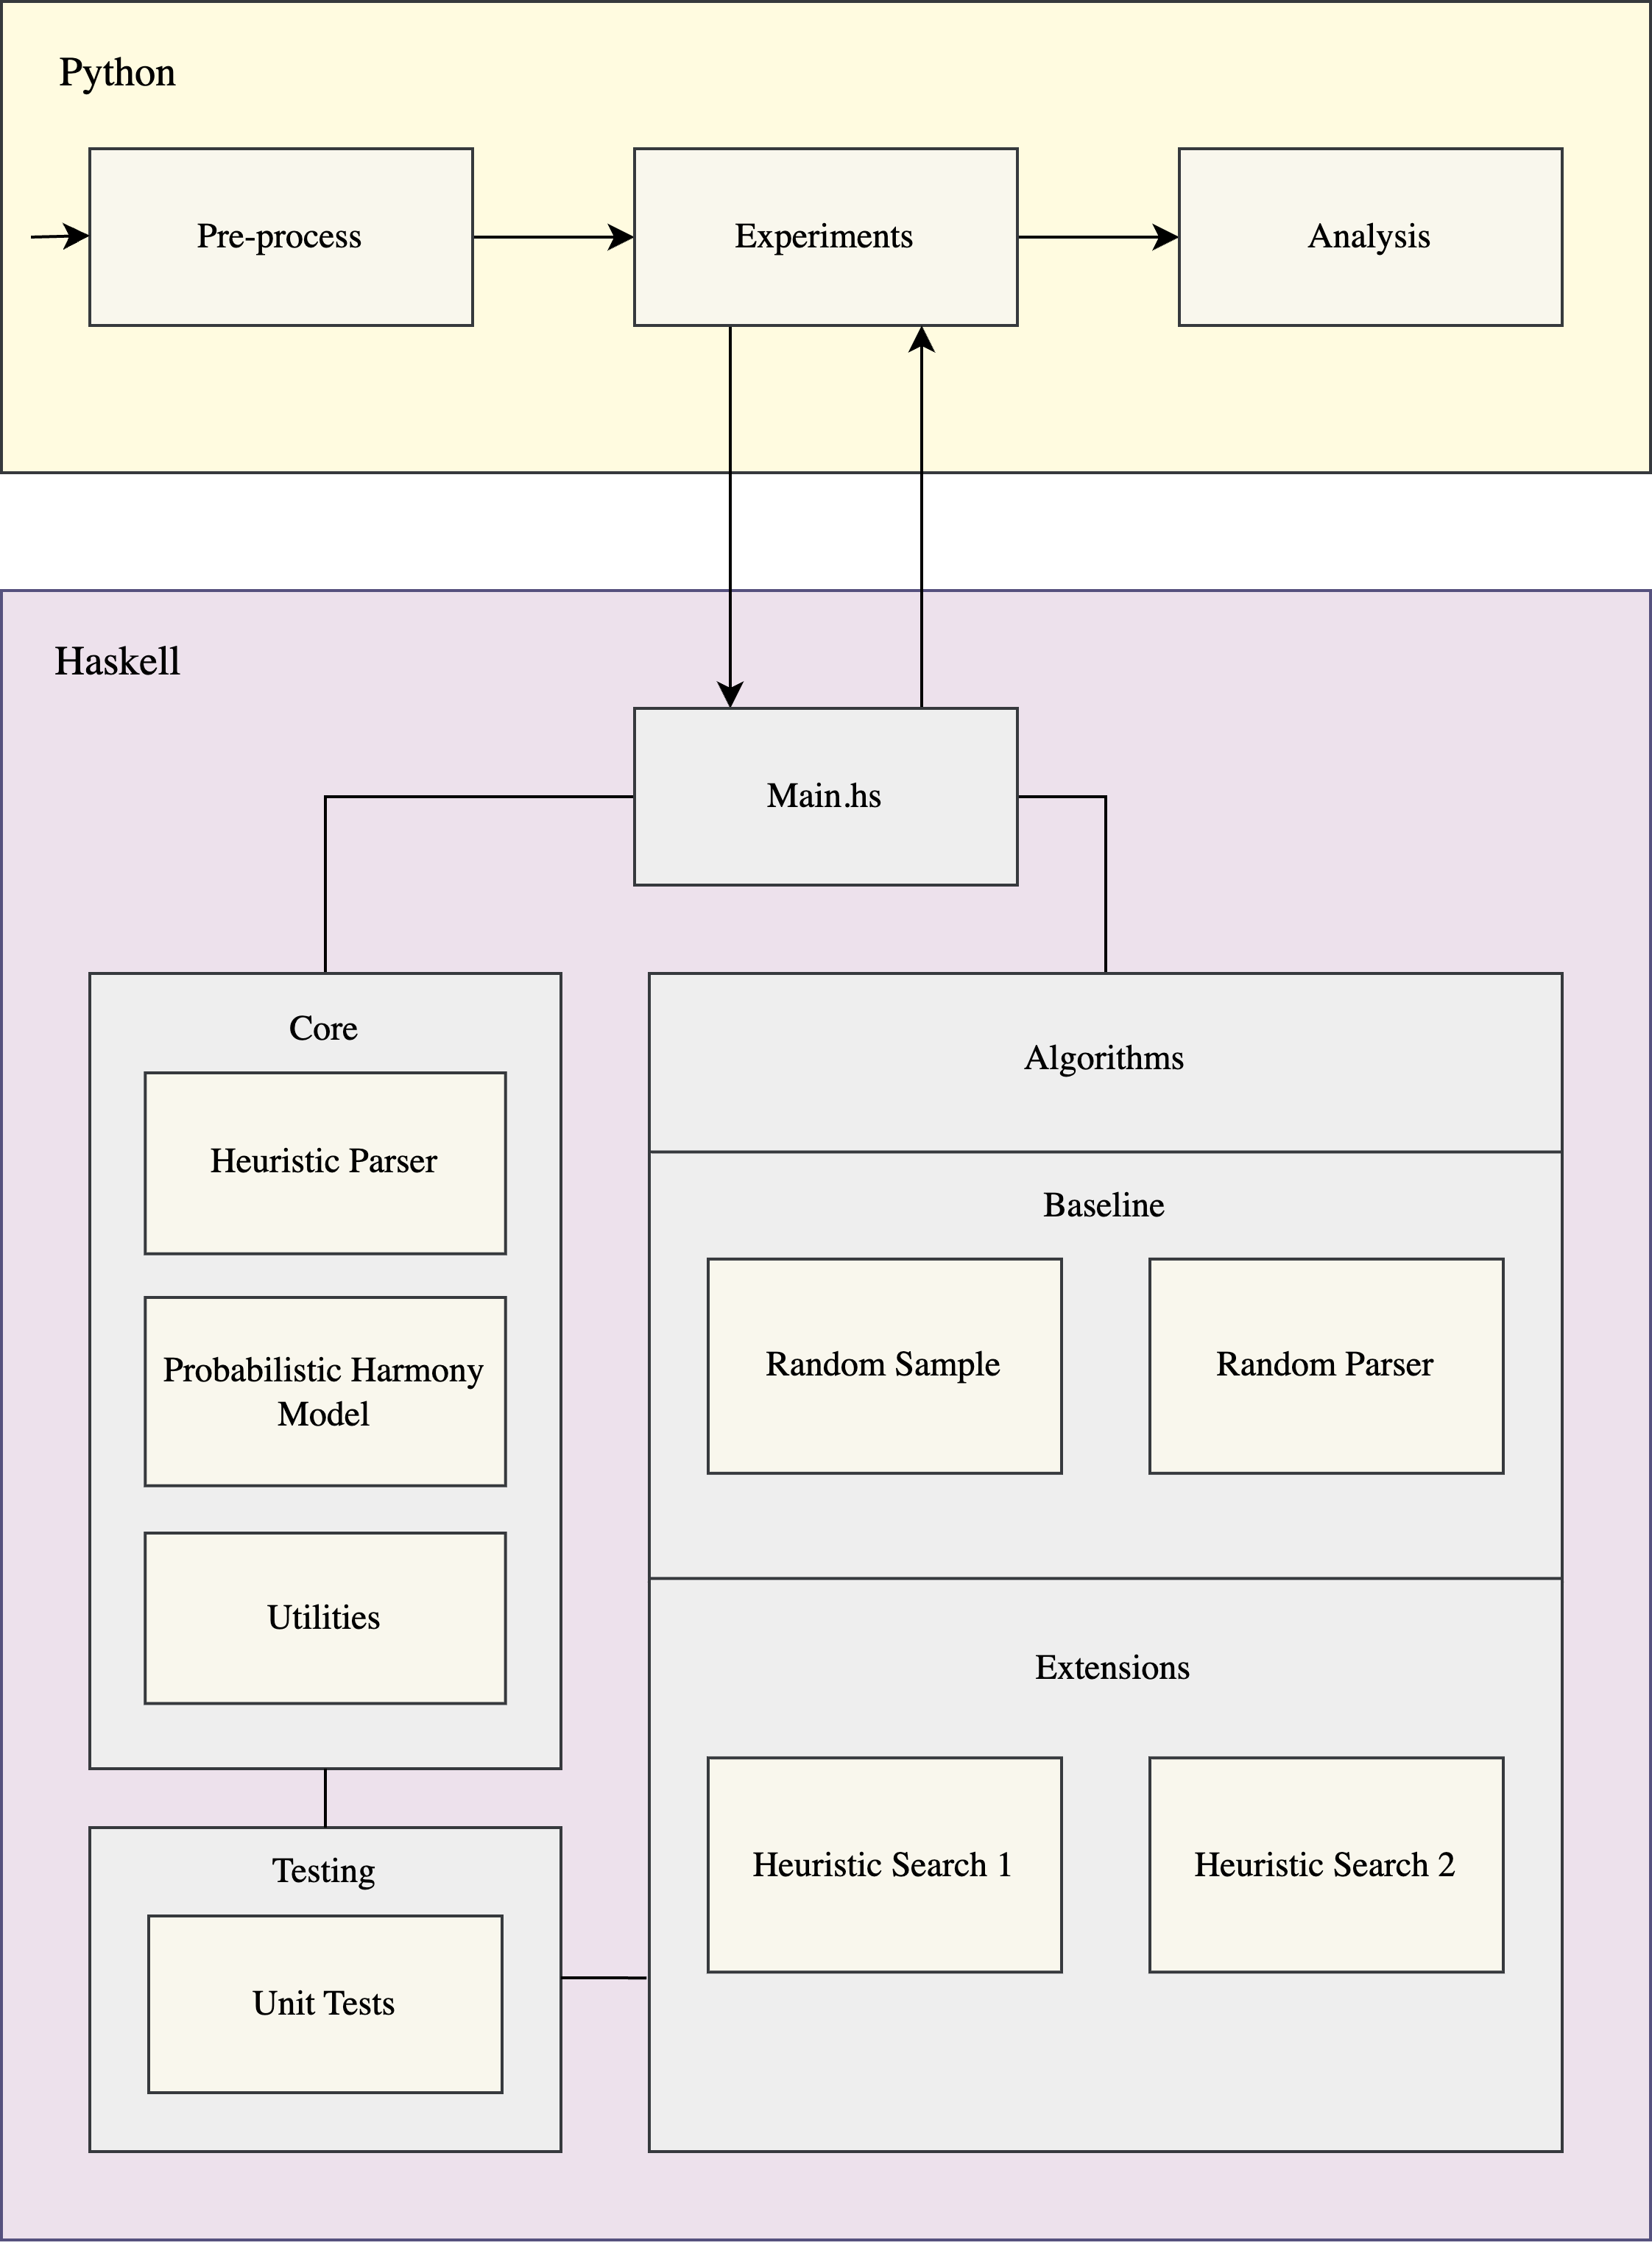
\includegraphics[width=\textwidth]{blockDiagram.png}
  \caption{Block diagram of project components}
  \label{fig:blockDiagram}
\end{figure}

{
\begin{table}[h]
  \DTsetlength{0em}{1.3em}{0em}{0.7pt}{3pt}       
  \setlength{\DTbaselineskip}{15pt}  %minimum size for \normalsize
  \renewcommand{\DTstyle}{\ttfamily}
  % \centering
  \caption{Repository Overview}
  \vspace{\baselineskip}
  \label{jeff}
  \begin{tabularx}{\textwidth}{l X c}
    File/Folder & Description & LOC \\
    \toprule
    \toprule
  \begin{minipage}[t]{5.3cm}
    \dirtree{%
    .1 protovoices-haskell/.
    .2 src/.
    .3 HeuristicParser.hs,~HeuristicSearch.hs \vspace{\DTbaselineskip}.
    .3 RandomChoiceSearch.hs,~RandomSampleParser.hs\vspace{2\DTbaselineskip}.
    .3 Heuristics.hs,~PBHModel.hs \vspace{2\DTbaselineskip}.
    .3 FileHandling.hs\vspace{2\DTbaselineskip}.
    .3 \dots \vspace{\DTbaselineskip}.
    .2 app/.
    .3 MainFullParse.hs\vspace{\DTbaselineskip}. 
    .2 harmonic-inference \vspace{\DTbaselineskip}.
    .2 experiments/.
    .3 preprocess.ipynb.
    .3 experiments.ipynb.
    .3 analysis.ipynb.
    .3 dcml\_params.json.
    .3 inputs/ \vspace{\DTbaselineskip}.
    .2 test/ \vspace{\DTbaselineskip}.
    }
  \end{minipage} &
  \begin{minipage}[t]{8cm}
Root directory
\vspace{2\baselineskip}\\
Core Implementation (Section x)
\vspace{2\baselineskip}\\
Baseline Implemetation (Section x)
\vspace{2\DTbaselineskip}\\
Extension Implementation (Section x) 
\vspace{2\DTbaselineskip}\\
Utilities
\vspace{5\DTbaselineskip}\\
Entry Point
\vspace{3\DTbaselineskip}\\
Running Experiments
\vspace{6\DTbaselineskip}\\
Unit Tests (Section x)

  \end{minipage} & 
  \begin{minipage}[t]{0.5cm}
    2272
    \vspace{0.1\DTbaselineskip}\\
    470\\
    \vspace{\DTbaselineskip}
    121\\
    \vspace{\DTbaselineskip}
    383\\
    \vspace{1.8\DTbaselineskip}
    188\\
    \vspace{3.7\DTbaselineskip}
    431\\
    \vspace{3\DTbaselineskip}
    115\\
    \vspace{2.5\DTbaselineskip}
    611\\
  \end{minipage}
\end{tabularx}
\end{table}
}

% The repository for this project is a fork of an existing repository that contains useful data-types and functions for working with the protovoice model \cite{finkensiepModelingInferringProtovoice2021}. Uses these allows for interoperability with other projects involving the model.

\FloatBarrier
\section{Core Implementation}


% \begin{itemize}
%   \item First we use the \textit{protovoice model} to \textit{reduce} a musical surface, simplifying the score by removing redundant notes from the surface, using domain specific knowledge to infer the most likely latent structure, $\hat{D}$, which is in turn used to infer the most likely reduced surface, $S'$.
%     % \footnote{We are relying on the assumption that this structure is somehow shared between the processes of composition, listening, and analysis. This is a fair assumption to make given they are all considering the same thing.}. 
%   \item Subsequently, using a \textit{harmony model} $P(S'|L)$ we find the conditional likelihood of the \textit{reduced} surface $S'$ given a hypothesised sequence of labels, $L$.
%   \item Finally, we choose the sequence of labels $\hat{L}$ that \textit{maximises the likelihood} of the reduced score.
% \end{itemize}
%
% We find a \textbf{reduction} of the original surface $S$, denoted $\hat{S'} = top(\argmax_D P(D|S))$
%
% The approach taken in the PVHM is as follows:
%
%
%
% The method I will use to infer harmony using the protovoice model is to find a plausible \textit{reduced surface} $S'$ which has one slice per chord label, having explicitly explained away non chord-tones (ornamentations) through protovoice edges. 
% Given this, the chord labels can be inferred using a model of harmony.
%


\subsection{End to End Pipeline}
The next step was to implement a full end-to-end pipeline from input to chord label predictions.
This was achieved writing \texttt{preprocessing.py}, \texttt{experiments.ipynb} and \texttt{analysis.ipynb}. This was then containerised using Docker, so that experiments could be run using a HPC. A jupyter-lab environment was set up to run the full pipeline.


\subsubsection{Data set selection}

The datasets used contain a selection or corpuses, bodies of work by a single composer as shown below, these were selected to exhibit a range of different styles. 
Each dataset contains an entire set work by a composer consisting of between $15-50$ annotated scores, each with varying lengths.

We divide each dataset into training, validation, and test sets, using a 60:20:20 split, using \textit{stratified sampling} in order to maintain a balanced representation of the different composers.

\subsubsection{Choosing Hyperparameters}

In order to choose hyperparameters, we combine the training and validation sets from each of the five datasets into a single training pool, then use 5-fold cross-validation using the training pool. 

\subsubsection{Final evaluation plan}

For the final evaluation, the performance of all developed algorithms will be evaluated on the hold-out test set (20\%). This is to provide an unbiased estimate of each algorithm's performance on \textbf{unseen} data.

We are also assessing the trade-off between accuracy and performance.

\subsection{Harmony Model}

The first step was to implement the harmony model that allows us to compute $P(L|S')$ and $P(L|S)$. This provides a framework to evaluate all developed algorithms. We use log probabilities.


\subsubsection{Predicting labels from reduced slices}
We have a set of pitches $\mathcal{P}$ and a set chord-types $\mathcal{C}$.
A chord label is defined as a tuple of \textit{root note} pitch and chord-type: $\mathcal{L} = (\mathcal{P}, \mathcal{C})$. 
Consider a slice $s = \left\{ p_1^{m(p_1)} , \dots, p_n^{m(p_n)} \right\}$ where $p_i \in \mathcal{P}$. We consider all possible chord labels $l \in \mathcal{L}$.
% We perform a transform of the pitches of each note relative to the chord's root note that is being considered, such that we only need to consider the chord type. 

The goal is to find:
\begin{equation}
  \hat{l} = \arg\max_l P(l|s)
  \label{eq:}
\end{equation}

We choose to find $P(s|l)$ rather than $P(s|l)$ as it gives us a \textit{confidence} in our prediction, given by $P(\hat{l}|s)$.

We first consider the simple case that all pitches in the slice $s$ are \textit{chord-tones} of the actual label.

We model the generation of a slice $s$ of size $n$ from a label $l$ as follows:

\begin{equation}
  \begin{gathered}
    % &$For $i \in 1 \dots n$ :$ \\
    &s \sim $Multinomial$(n, |\mathcal{P}|,\bm{\Phi}_l)\\
    &$where $\bm{\phi}_{l}^{(p)} = P($Pitch $=p | $Label $=l)\\ 
    % &$where $\bm{\phi}^T = \left[\bm{\phi}_{1}~~\bm{\phi}_{2}~~\dots~~\bm{\phi}_{|L|} \right]\ 
    % &$and $\bm{\phi_} = \left[\bm{\phi}_{1}~~\bm{\phi}_{2}~~\dots~~\bm{\phi}_{|L|} \right]\ 
  \end{gathered}
  \label{eq:sliceModel}
\end{equation}

We define the slice vector $\bm{v}(s) = \left[~m(p_1)~ m(p_2)~\dots~m(p_{k})~\right]$ where $k = |\mathcal{P}|$. Then $P(l|s)$ is given by: 
\footnote{Struggling with naming here. Using $P$ for pitches conflicts the $P$ for probability.  }
\begin{equation}
  \begin{gathered}
    \begin{aligned}
      P(l|s) &= P(s|l)\cdot P(l) \\
             &= f(\bm{v}(s), \bm{\phi}_l)\cdot P(l) \\
    \end{aligned} \\
    \text{where $f$ is the multinomial probability density function} \\ 
    f(x_1, \dots, x_k;p_1, \dots, p_k) = \frac{\Gamma \left(\sum\limits_{i} x_i + 1 \right)}{\prod\limits_{i} \Gamma \left(x_i + 1\right)}~\prod\limits_{i=1}^{k} p_{i}^{x_i}
  \end{gathered}
  \label{eq:labelgivenchordtones}
\end{equation}

The log probability $\log P(l|s)$ is given by 
\begin{equation}
  \begin{align}
    \log P(l|s) &= \log P(s|l) + \log P(l) \\      
                &= \cdots \\
                &= \log \left(\Gamma\left(\sum\limits_{i} x_i + 1\right) \right) 
                +  \sum\limits \left( x_i \log p_i^{x_i} - \log \Gamma (x_i + 1) \right) 
                +  \log P(l)
  \end{align}
  \label{eq:loglabelgivenchordtones}
\end{equation}

So to find the most likely label $l$ given slice $s$ we take:
\begin{equation}
  \hat{l} = \arg\max_l \left(\log \left(\Gamma\left(\sum\limits_{i} x_i + 1\right) \right) 
                +  \sum\limits \left( x_i \log p_i^{x_i} - \log \Gamma (x_i + 1) \right) 
                +  \log P(l) \right)
  \label{eq:loglabsol}
\end{equation}

 %  | otherwise = logFactorialN + logPowers
 % where
 %  n = sum xs
 %  logFactorialN = logGamma $ n + 1
 %  logPowers = sum $ zipWith powers xs probs
 %   where
 %    powers x y = x * log y - logGamma (x + 1)

The full derivation has been omitted for the sake of brevity. Given that $|\mathcal{P}|$ is finite ($30$? I forgot) we can solve this directly. 

\subsubsection{Predicting chordness}
This is to guide the heuristic search.

We define \textit{chordness} as the likelihood that a given slice could have been generated by the most likely label $\hat{l}$.

\begin{equation}
  \text{Chordness}(s) = P(s | \hat{l}) P(\hat{l} | s) 
  \label{eq:chordness}
\end{equation}
where $\hat{l} = \argmax_l P(l | s)$ as above.

% Given whether or not each pitch is a chord-tone is independent, we can find $\sum\limits_{p\in s} P(p | l) = \sum\limits_{p \in s} \bm{\phi}$

% The parameters are as follows:
% \begin{itemize}
%   \item $\bm{\lambda}$
%   \item $\bm{\mu}$
%   \item $\bm{\nu}$
%   \item $\bm{\xi}$
%   \item $\bm{\chi}$
%   \item $\bm{\psi}$
% \end{itemize}
%
% Thus to find $P(s|l)$ we evaluate the multinomial probability density function 
%
%
% \begin{equation}
% \begin{align*} 
%               && \vec{\chi} &\sim \text{Dirichlet}(0.5, |\mathcal{C}|)     && \text{prior of the chord type} \\
%               && \lambda &\sim \text{Gamma}(3, 1)     && \text{prior of the note rate} \\
%   \forall c:  && \theta_c  &\sim \text{Beta}(1, 1)        && \text{prior of each note being a chordtone/ ornament} \\
%   \forall c:  && \vec{\phi}_{ct}^{c}  &\sim \text{Dirichlet}(0.5, |\mathcal{P}|)        && \text{pitch for each ornament} \\
%   \forall c:  && \vec{\phi}_{or}^{c}  &\sim \text{Dirichlet}(0.5, |\mathcal{P}|)        && \text{pitch for each chord tone} \\
%   % \forall i:  && L_i | \vec{\chi} &\sim \text{Categorical}(\vec{\chi}) && \text{chord label of each data point} \\
%   %             && N_i | L_i, v &\sim \text{Multinomial}(v_{L_i})  && \text{notes of each data point} \\
% \end{align*}
% \label{eq:phm}
% \end{equation}
%
%
%
% \par
% The priors for the model are as follows:
% \begin{equation}
% \begin{align*} 
%               && \vec{\chi} &\sim \text{Dirichlet}(0.5, |\mathcal{C}|)     && \text{prior of the chord type} \\
%               && \lambda &\sim \text{Gamma}(3, 1)     && \text{prior of the note rate} \\
%   \forall c:  && \theta_c  &\sim \text{Beta}(1, 1)        && \text{prior of each note being a chordtone/ ornament} \\
%   \forall c:  && \vec{\phi}_{ct}^{c}  &\sim \text{Dirichlet}(0.5, |\mathcal{P}|)        && \text{pitch for each ornament} \\
%   \forall c:  && \vec{\phi}_{or}^{c}  &\sim \text{Dirichlet}(0.5, |\mathcal{P}|)        && \text{pitch for each chord tone} \\
%   % \forall i:  && L_i | \vec{\chi} &\sim \text{Categorical}(\vec{\chi}) && \text{chord label of each data point} \\
%   %             && N_i | L_i, v &\sim \text{Multinomial}(v_{L_i})  && \text{notes of each data point} \\
% \end{align*}
% \label{eq:phm}
% \end{equation}
% \par 
% Given this model we use it to generate a single chord as follows:
%
% \par
% Then describe how to go from the parameters to chord, chordtone and ornamentation distributions
% \par

% \subsubsection{Model inference}
% Given the model, we use a dataset to learn the parameters of the model. These parameters can then be used for inference as follows.
% For each datapoint, the chord label 
% \begin{equation}
% \begin{align*} 
%   \forall i:  && L_i | \vec{\chi} &\sim \text{Categorical}(\vec{\chi}) && \text{chord label of each data point} \\
%               && N_i | L_i, v &\sim \text{Multinomial}(v_{L_i})  && \text{notes of each data point} \\
% \end{align*}
% \label{eq:chordlabeldp}
% \end{equation}
%
% \par

% Chordtypes, $C = \{\text{M,~m, Mm7, om, o7, mm7, \%7, MM7, +, Ger, It, Fr, mM7, +7}\}$
%
% \[\vec{\chi}' \sim \text{Dirchlet} (\text{pHarmonies}, n_c) \]
%
% \[\vec{\chi} = \mathbb{E} (\vec{X}_i) = \frac{\alpha_i}{\sum\limits_j \alpha_j} \]
%
% Chord: \[c \sim \text{Categorical}(\vec{\chi})\]
%
% Single chordtone distribution. We want to find $P(p|c, ct)$ probability of the pitch given the chord, and that the note is a chordtone:
% \[\vec{\phi}_{ct}' \sim \text{Dirchlet}(pChordtones, n_p) \implies \vec{\phi}\]
%
% For each of these parameters we use the MLE to get our probability distribution. 
% \[\vec{\phi}_{ct} = \text{MLE} (\vec{\phi}_{ct}')\]
% \[\vec{\phi}_{or} = \text{MLE} (\vec{\phi}_{or}')\]
% \[\vec{\chi}= \text{MLE} (\vec{\chi}') \]
% Then for each chord tone,
% \[p_{ct} \sim \text{Categorical}(\vec{\phi}_{ct})\]
% \[p_{or} \sim \text{Categorical}(\vec{\phi}_{or})\]
% We get the distribution of likelihoods for each pitch.
%
%
% Provide an outline of the heuristic search paradigm with a formalisation.
% \par
% Provide a brief overview of different techniques that are used to prune the search space that might be relevant.

\subsection{Protovoice Parser}

The goal of this section is to construct a parser for the protovoice model $S \to D$. We represent each step as a \texttt{state} and implement \texttt{expand(state)} such that we can use search algorithms to conduct the parse.

\subsubsection{Parse state}

We will represent the state as a path graph, and construct a \textit{leftmost} derivation of the surface given protovoice operations.

\begin{figure}[h]
  \centering
  \begin{subfigure}[t]{\textwidth}
    \centering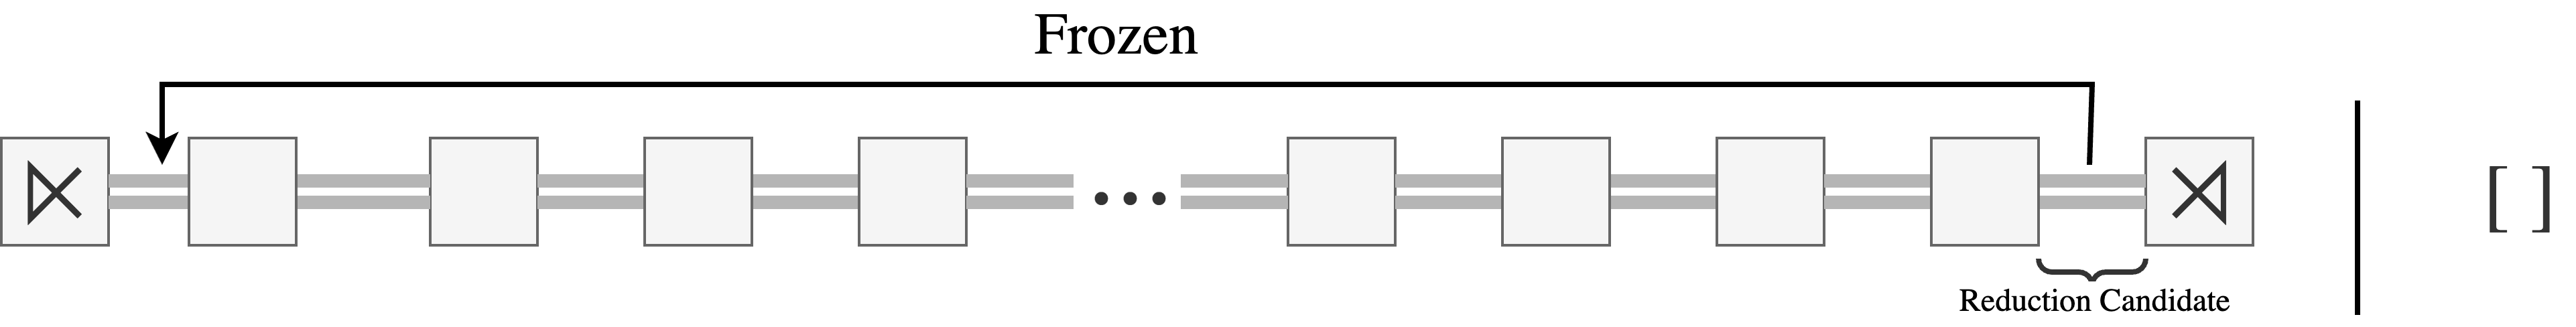
\includegraphics[keepaspectratio,width=\textwidth]{impl/parseState/frozen}
    \caption{\texttt{SSFrozen}}
    \label{fig:ssfrozen}
  \end{subfigure}
  \begin{subfigure}[t]{\textwidth}
    \centering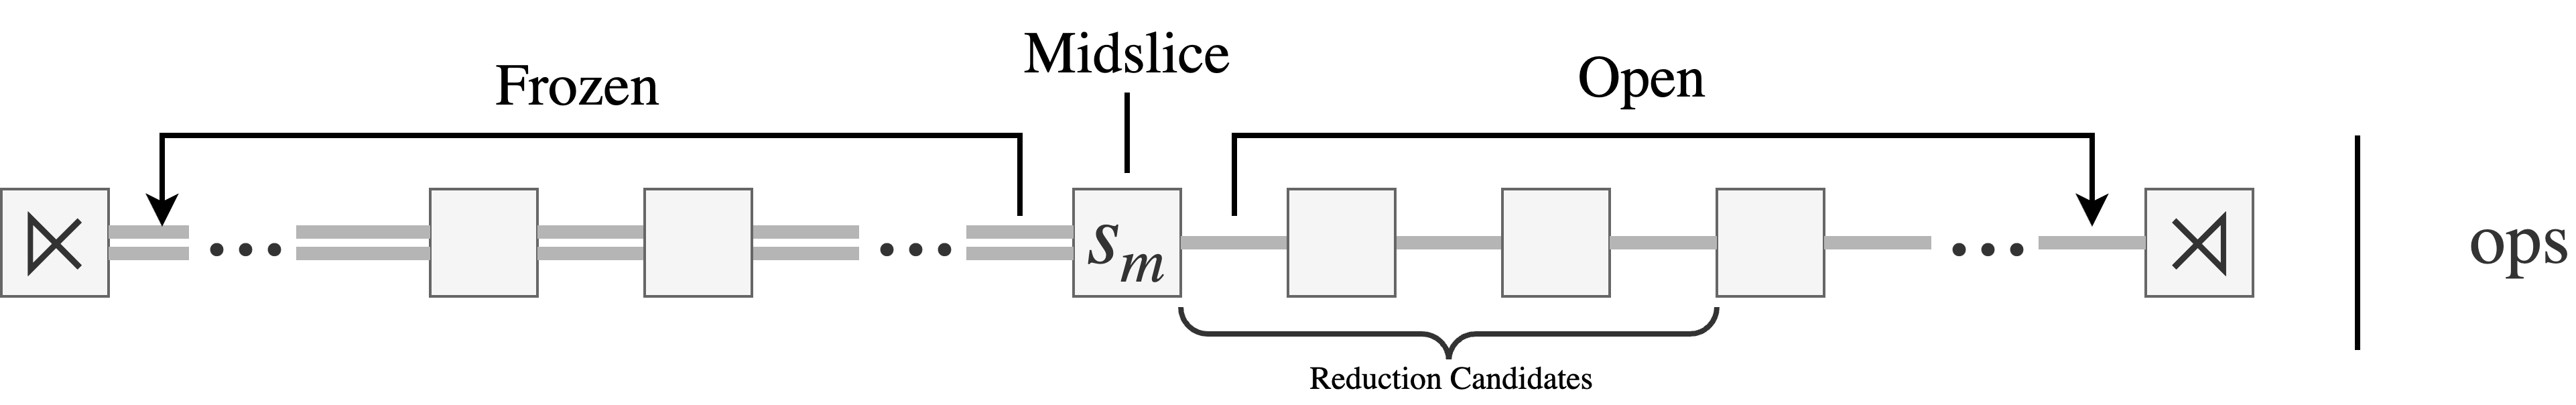
\includegraphics[keepaspectratio,width=\textwidth]{impl/parseState/semiopen}
    \caption{\texttt{SSSemiOpen}}
    \label{fig:sssemiopen}
  \end{subfigure}
  \begin{subfigure}[t]{\textwidth}
    \centering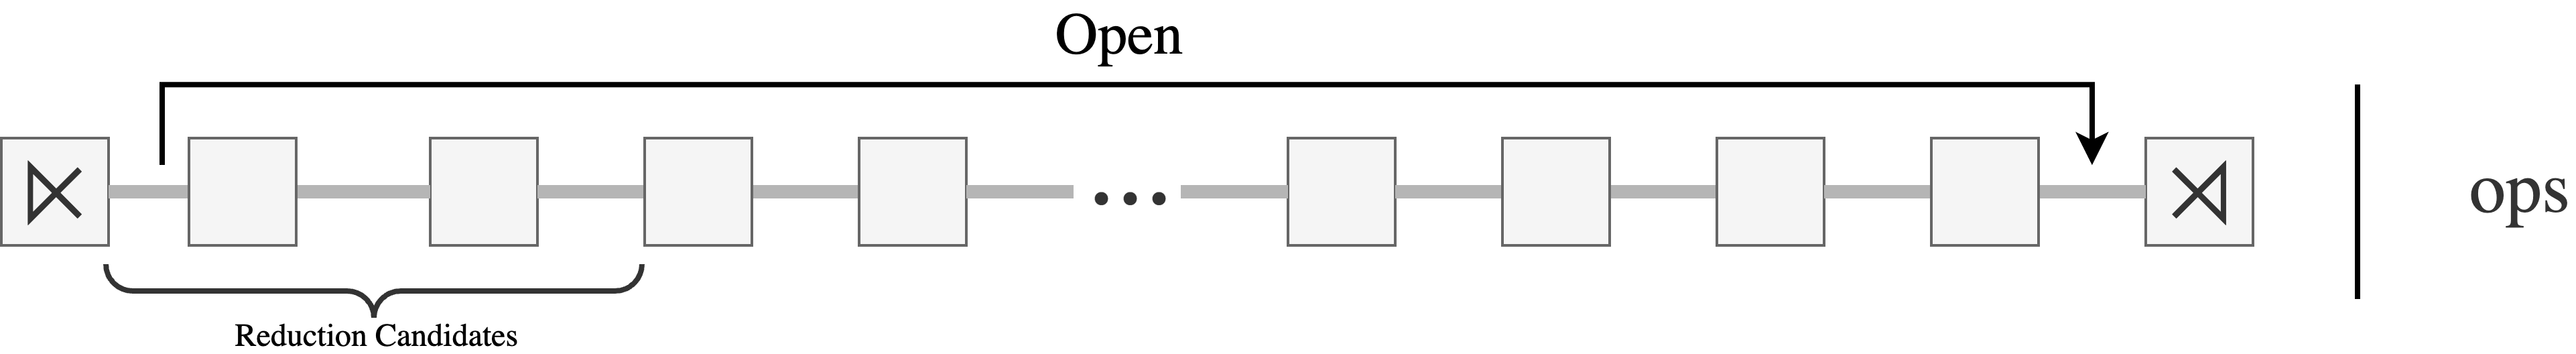
\includegraphics[keepaspectratio,width=\textwidth]{impl/parseState/open}
    \caption{\texttt{SSFrozen}}
    \label{fig:ssfrozen}
  \end{subfigure}
  \captionsetup{width=.9\linewidth}
  \caption{Parse states}
  \label{fig:parseState}
\end{figure}

We begin in the frozen state, at the end of the piece.

This is how we define the search. We start at the right, the end of the piece. We have a pointer to the current node, and all preceeding slices are open and subsequent slices are frozen. Open Slices can be reduced, but only to the point that there is one slice in a segment. We keep track of the operations performed as it (1). allows us to the draw out the derivation for the partial reduction at the end, and (2). it is used later for calculate a cost for each operation for the heuristic search.



\begin{lstlisting}[caption={protovoiceEvaluator}, captionpos=b]
data SearchState es es' ns o
  = SSFrozen !(Path (Maybe es', Bool) (SliceWrapped ns)) 
  -- ^ Beginning of search - all frozen edges and slices
  | SSSemiOpen 
  -- ^ Mid-search
      { _ssFrozen :: !(Path (Maybe es', Bool) (SliceWrapped ns))
      -- ^ frozen transitions and slices from current point leftward
      , _ssMidSlice :: !(SliceWrapped ns)
      -- ^ the slice at the current posision between gsFrozen and gsOpen
      , _ssOpen :: !(Path (Trans es) (SliceWrapped ns))
      -- ^ non-frozen transitions and slices from current point rightward
      , _ssDeriv :: ![o]
      -- ^ derivation from current reduction to original surface
      }
  | SSOpen !(Path (Trans es) (SliceWrapped ns)) ![o] 
  -- ^ Single path with unfrozen transition,slices and history
\end{lstlisting}
\footnote{This should be changed to \texttt{ParseState}}

Decision as to how to run the parse. We choose have a single point of reduction to lower the number of options at each step.
There were three choices as to how to run the parse:
\begin{itemize}
  \item Free derivation: Given that the reductions can be applied to arbitrary 
  \item Right-most derivation:  
  \item Left-most derivation: blah blah, we choose to do this because 
\end{itemize}


\subsubsection{Parsing Operations}
The \texttt{protoVoiceEvaluator} \cite{finkensiepModelingInferringProtovoice2021} provides an interface for the following functions. This code has been simplified in order to omit details:

\begin{figure}[h]
  \centering
  \begin{subfigure}[t]{.2\textwidth}
    \centering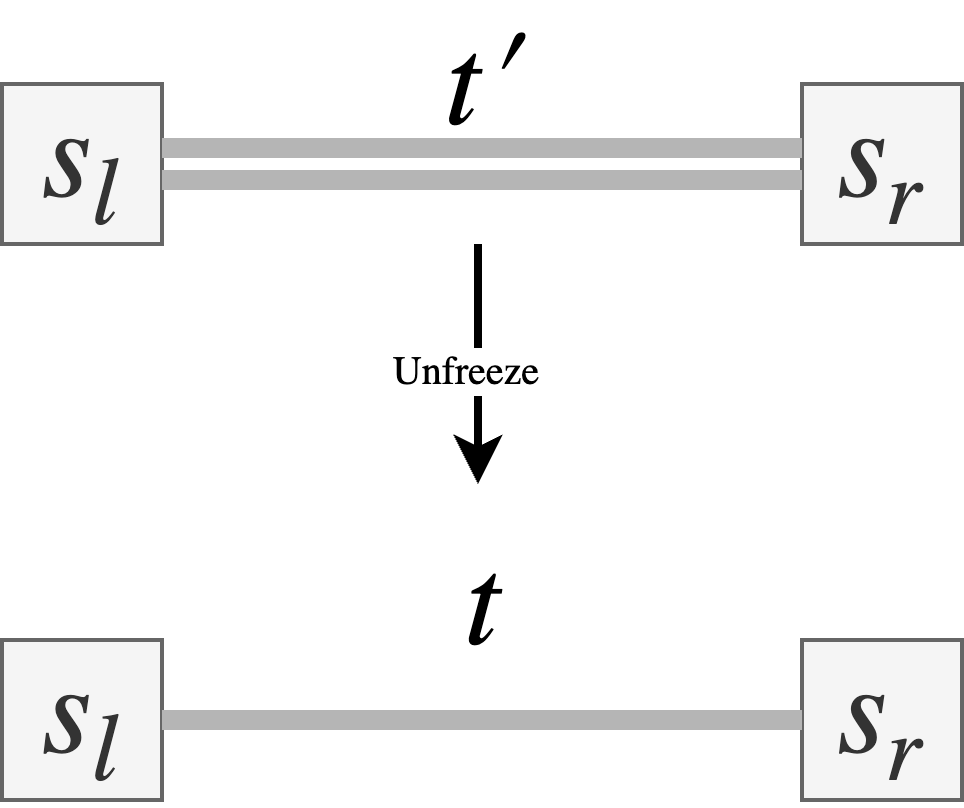
\includegraphics[keepaspectratio,width=\textwidth]{impl/eval/unfreeze}
    \caption{\texttt{Unfreeze}}
    \label{fig:splitOp}
  \end{subfigure}
  \begin{subfigure}[t]{.43\textwidth}
    \centering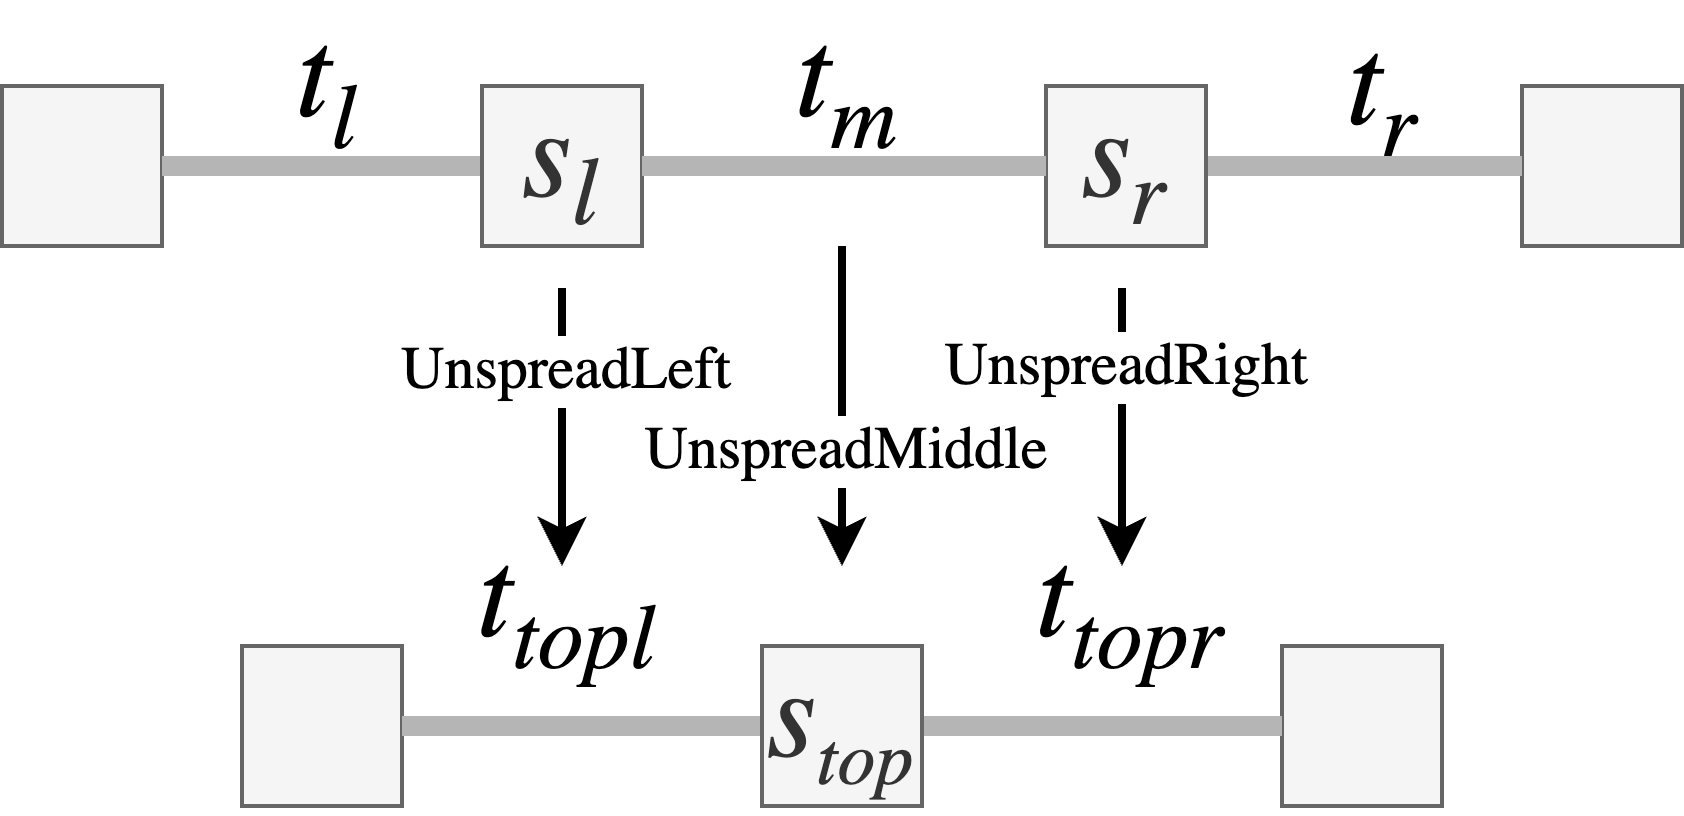
\includegraphics[keepaspectratio,width=0.8\textwidth]{impl/eval/unspread}
    \caption{\texttt{Unspread}}
    \label{fig:spreadOP}
  \end{subfigure}
  \begin{subfigure}[t]{.3\textwidth}
    \centering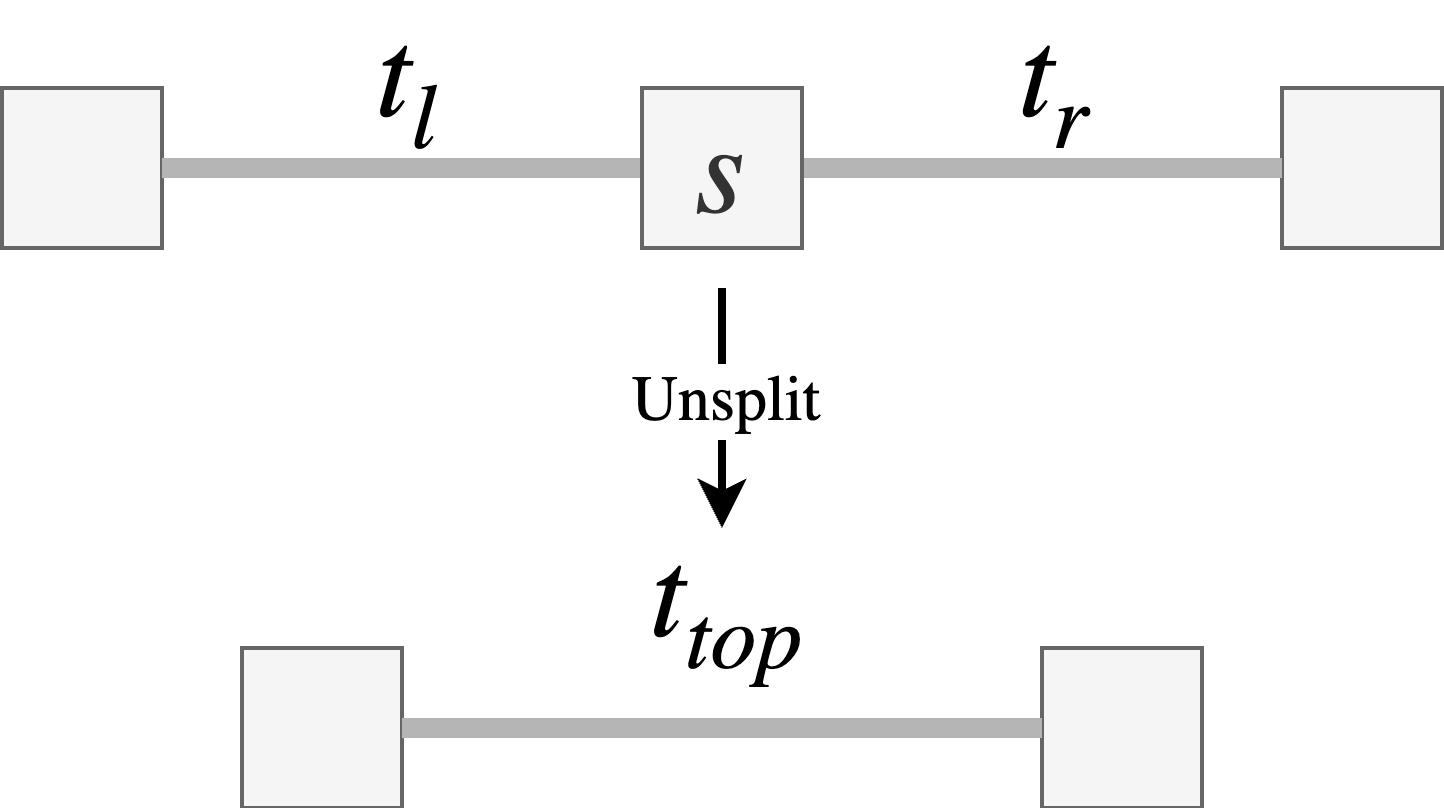
\includegraphics[keepaspectratio,width=\textwidth]{impl/eval/unsplit}
    \caption{\texttt{Unsplit}}
    \label{fig:freezeOp}
  \end{subfigure}

  \captionsetup{width=.9\linewidth}
  \caption{Reduction operations.}
  \label{fig:evalOps}
\end{figure}

\begin{lstlisting}

type UnspreadMiddle tr slc v = 
  (slc, tr, slc) -> Maybe (slc, v)

type UnspreadLeft tr slc = 
  (tr, slc) -> slc -> [tr]

type UnspreadRight tr slc = 
  (slc, tr) -> slc -> [tr]

type Unsplit tr slc v =
  StartStop slc -> tr -> slc -> tr -> StartStop slc -> SplitType -> [(tr, v)]

type Unfreeze tr' tr slc =
  StartStop slc -> Maybe tr' -> StartStop slc -> [(tr, v)]
\end{lstlisting}

Transition can be frozen or unfrozen, and boundary or non boundary. Boundary is represented by vertical line, frozen is represented by two lines.

\subsubsection{Boundary handling}

The goal of the parse is to reduce the surface such that there is one slice per segment. 

In order to achieve this we impose constraints on which reduction operations can be performed, dependent on adjacent segment boundaries. 

Each transition has a boolean boundary value which indicates if the transition is across a segment boundary. We use karnaugh maps to determine the boolean expression for these constraints. 
Let $B_f$, $B_l$, $B_m$, and $B_r$ denote the boundary values of $t_f$, $t_l$, $t_m$ and $t_r$ respectively.

\begin{figure}[h]
  \begin{center}
    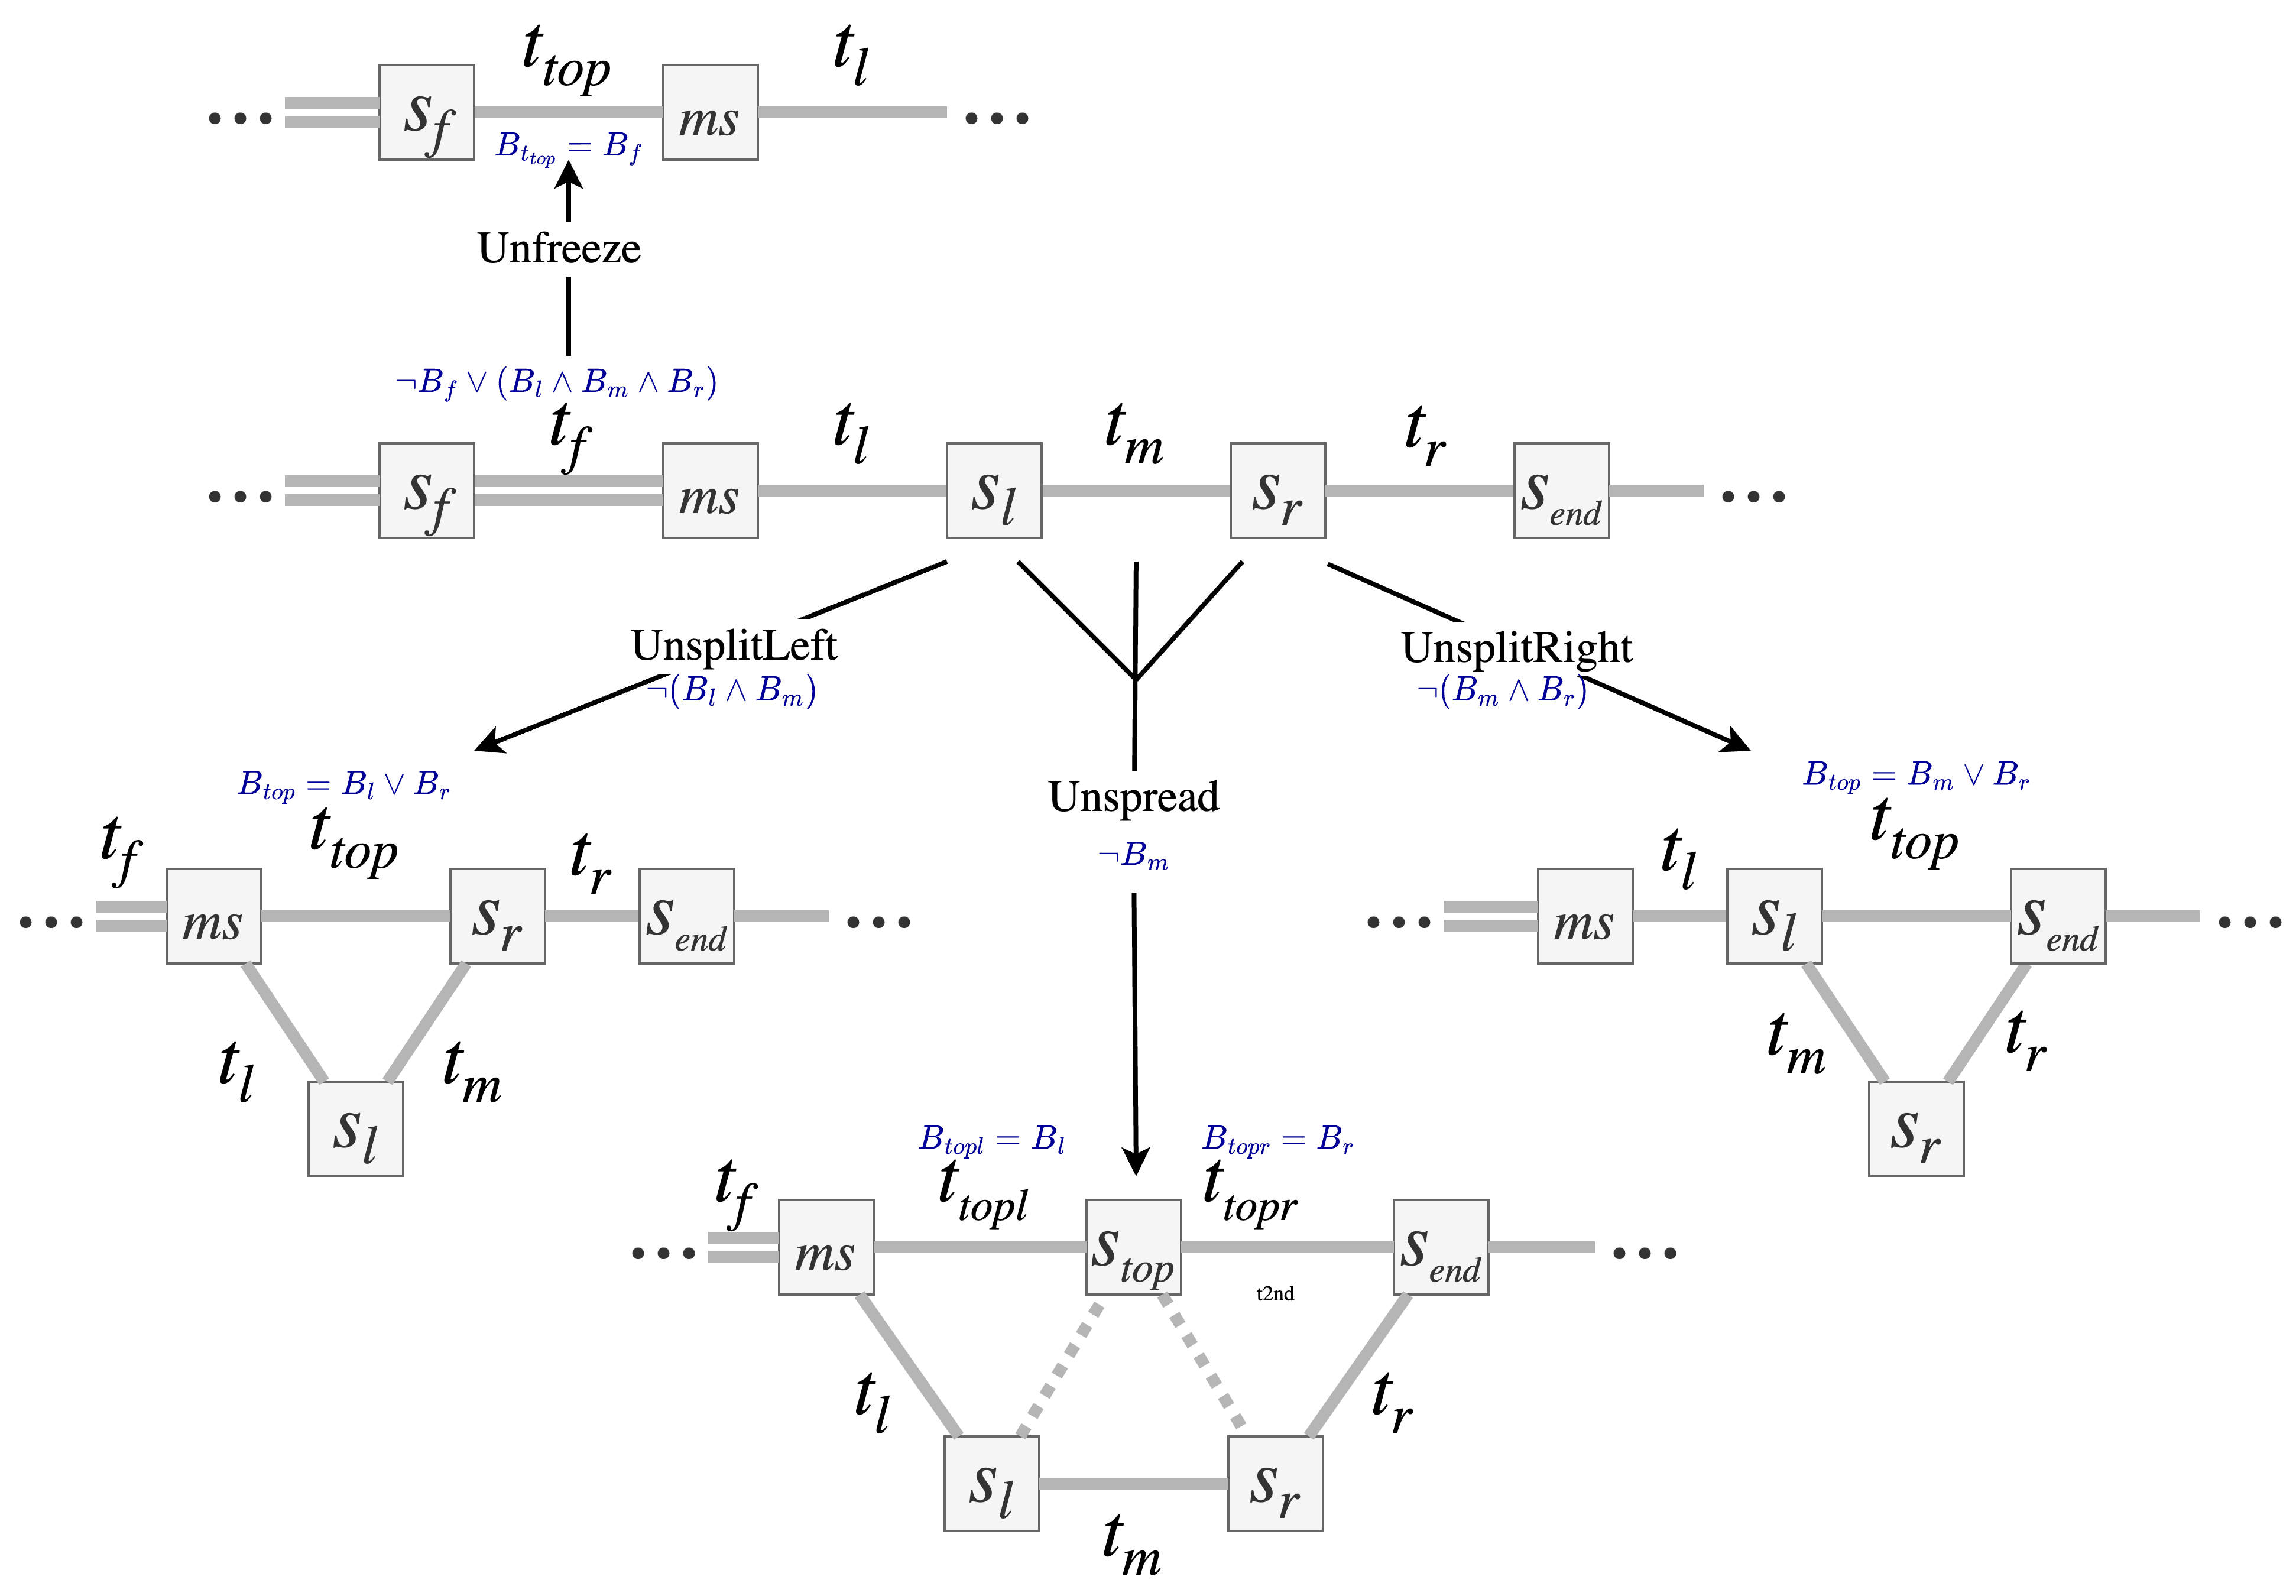
\includegraphics[width=0.75\textwidth]{impl/boundarydiagram/diag}
  \end{center}
  \caption{General Parse state}
  \label{fig:parseStateBound}
\end{figure}

\begin{figure}[h]
  \centering
  \begin{subfigure}[t]{0.73\textwidth}
    \centering
    \begin{karnaugh-map}[4][2][1][$B_f$][$B_l$][$B_m$]
      \end{karnaugh-map}
    \caption{Unfreeze}
    \label{fig:unfreezeKarn}
  \end{subfigure}
  \begin{subfigure}[t]{0.65\textwidth}
    \centering
    \begin{karnaugh-map}[4][4][1][$B_f$][$B_l$][$B_m$][$B_r]
      \end{karnaugh-map}
    \caption{Unsplit}
    \label{fig:unfreezeKarn}
  \end{subfigure}
  \begin{subfigure}[t]{0.3\textwidth}
    \centering
      \begin{karnaugh-map}[4][4][1][$B_f$][$B_l$][$B_m$][$B_r]
      \end{karnaugh-map}
    \caption{Unspread}
    \label{fig:unfreezeKarn}
  \end{subfigure}
  \caption{Boundary constraints}
  \label{fig:boundaryKarn}
\end{figure}

\subsubsection{Initialising the parse}
The input consists of a list of slices, each with a boolean \texttt{Boundary} value which indicates if the given slice is the beginning of a new segment. 

\begin{figure}[h]
  \centering
  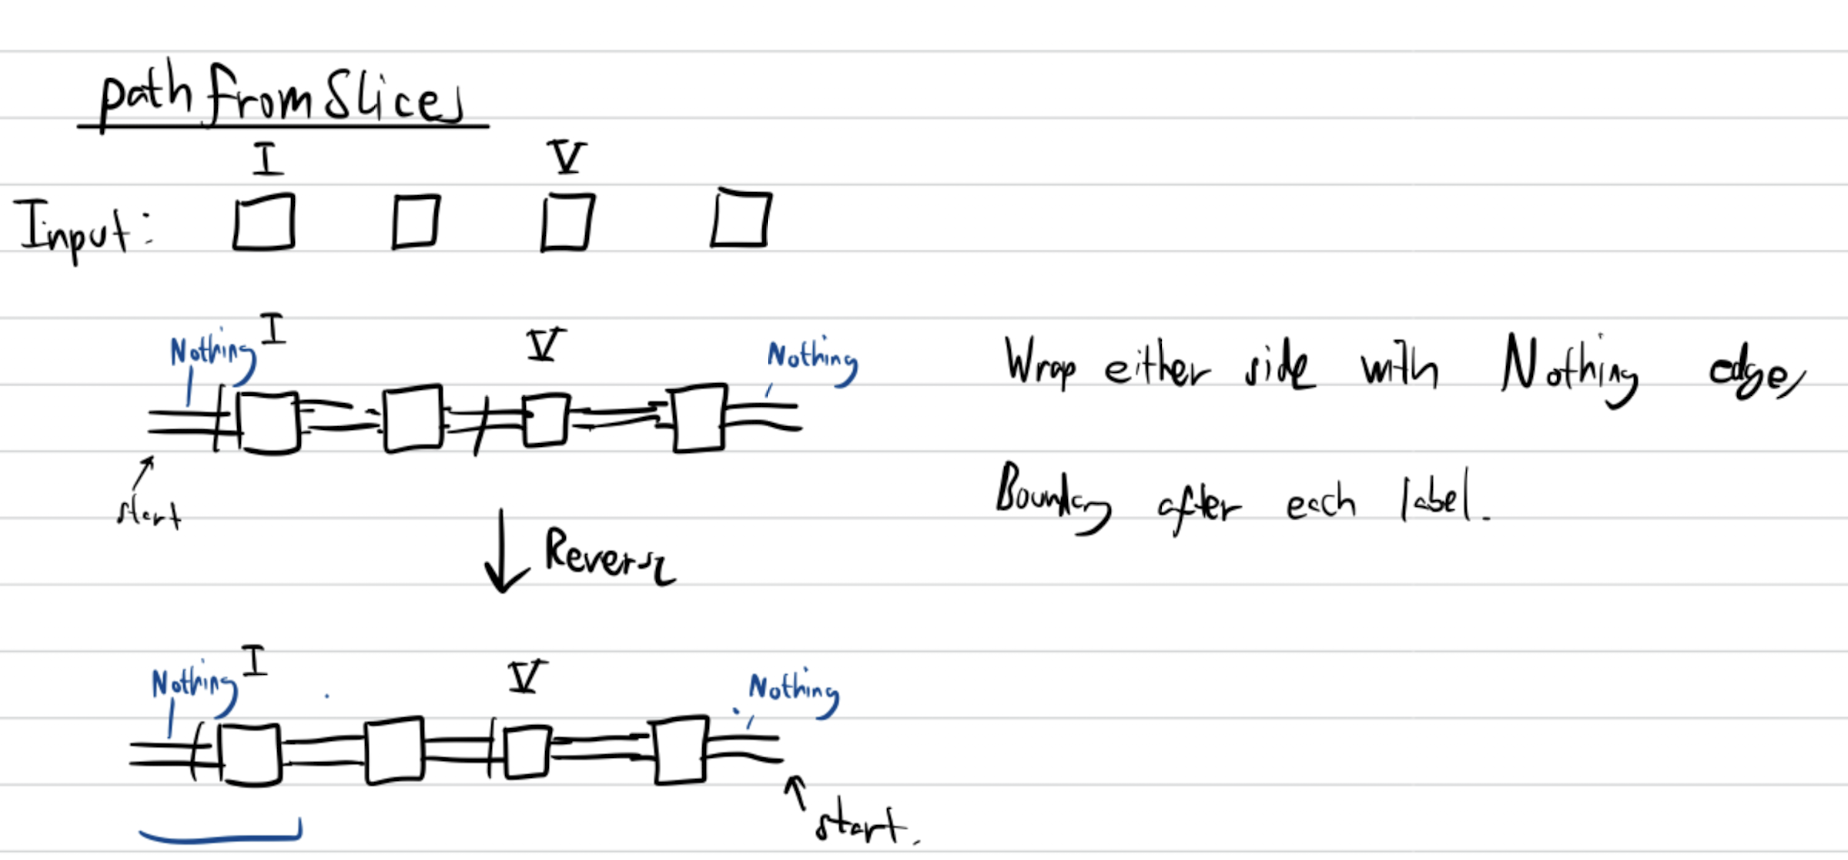
\includegraphics[width=0.6\textwidth]{pathFromSlices}
  \caption{Parse Initialisation}
  \label{fig:parseInit}
\end{figure}



\subsubsection{Parse Steps}

Figure~\ref{fig:parseStateOptions} shows the possible reductions in the general case. There are 4 options, but for each operation there are multiple inner reductions. EG for an unsplit ... 

The cases for open and frozen and when there aren't 3+ open transitions has to be considered very carefully.

\begin{figure}[h]
  \centering
  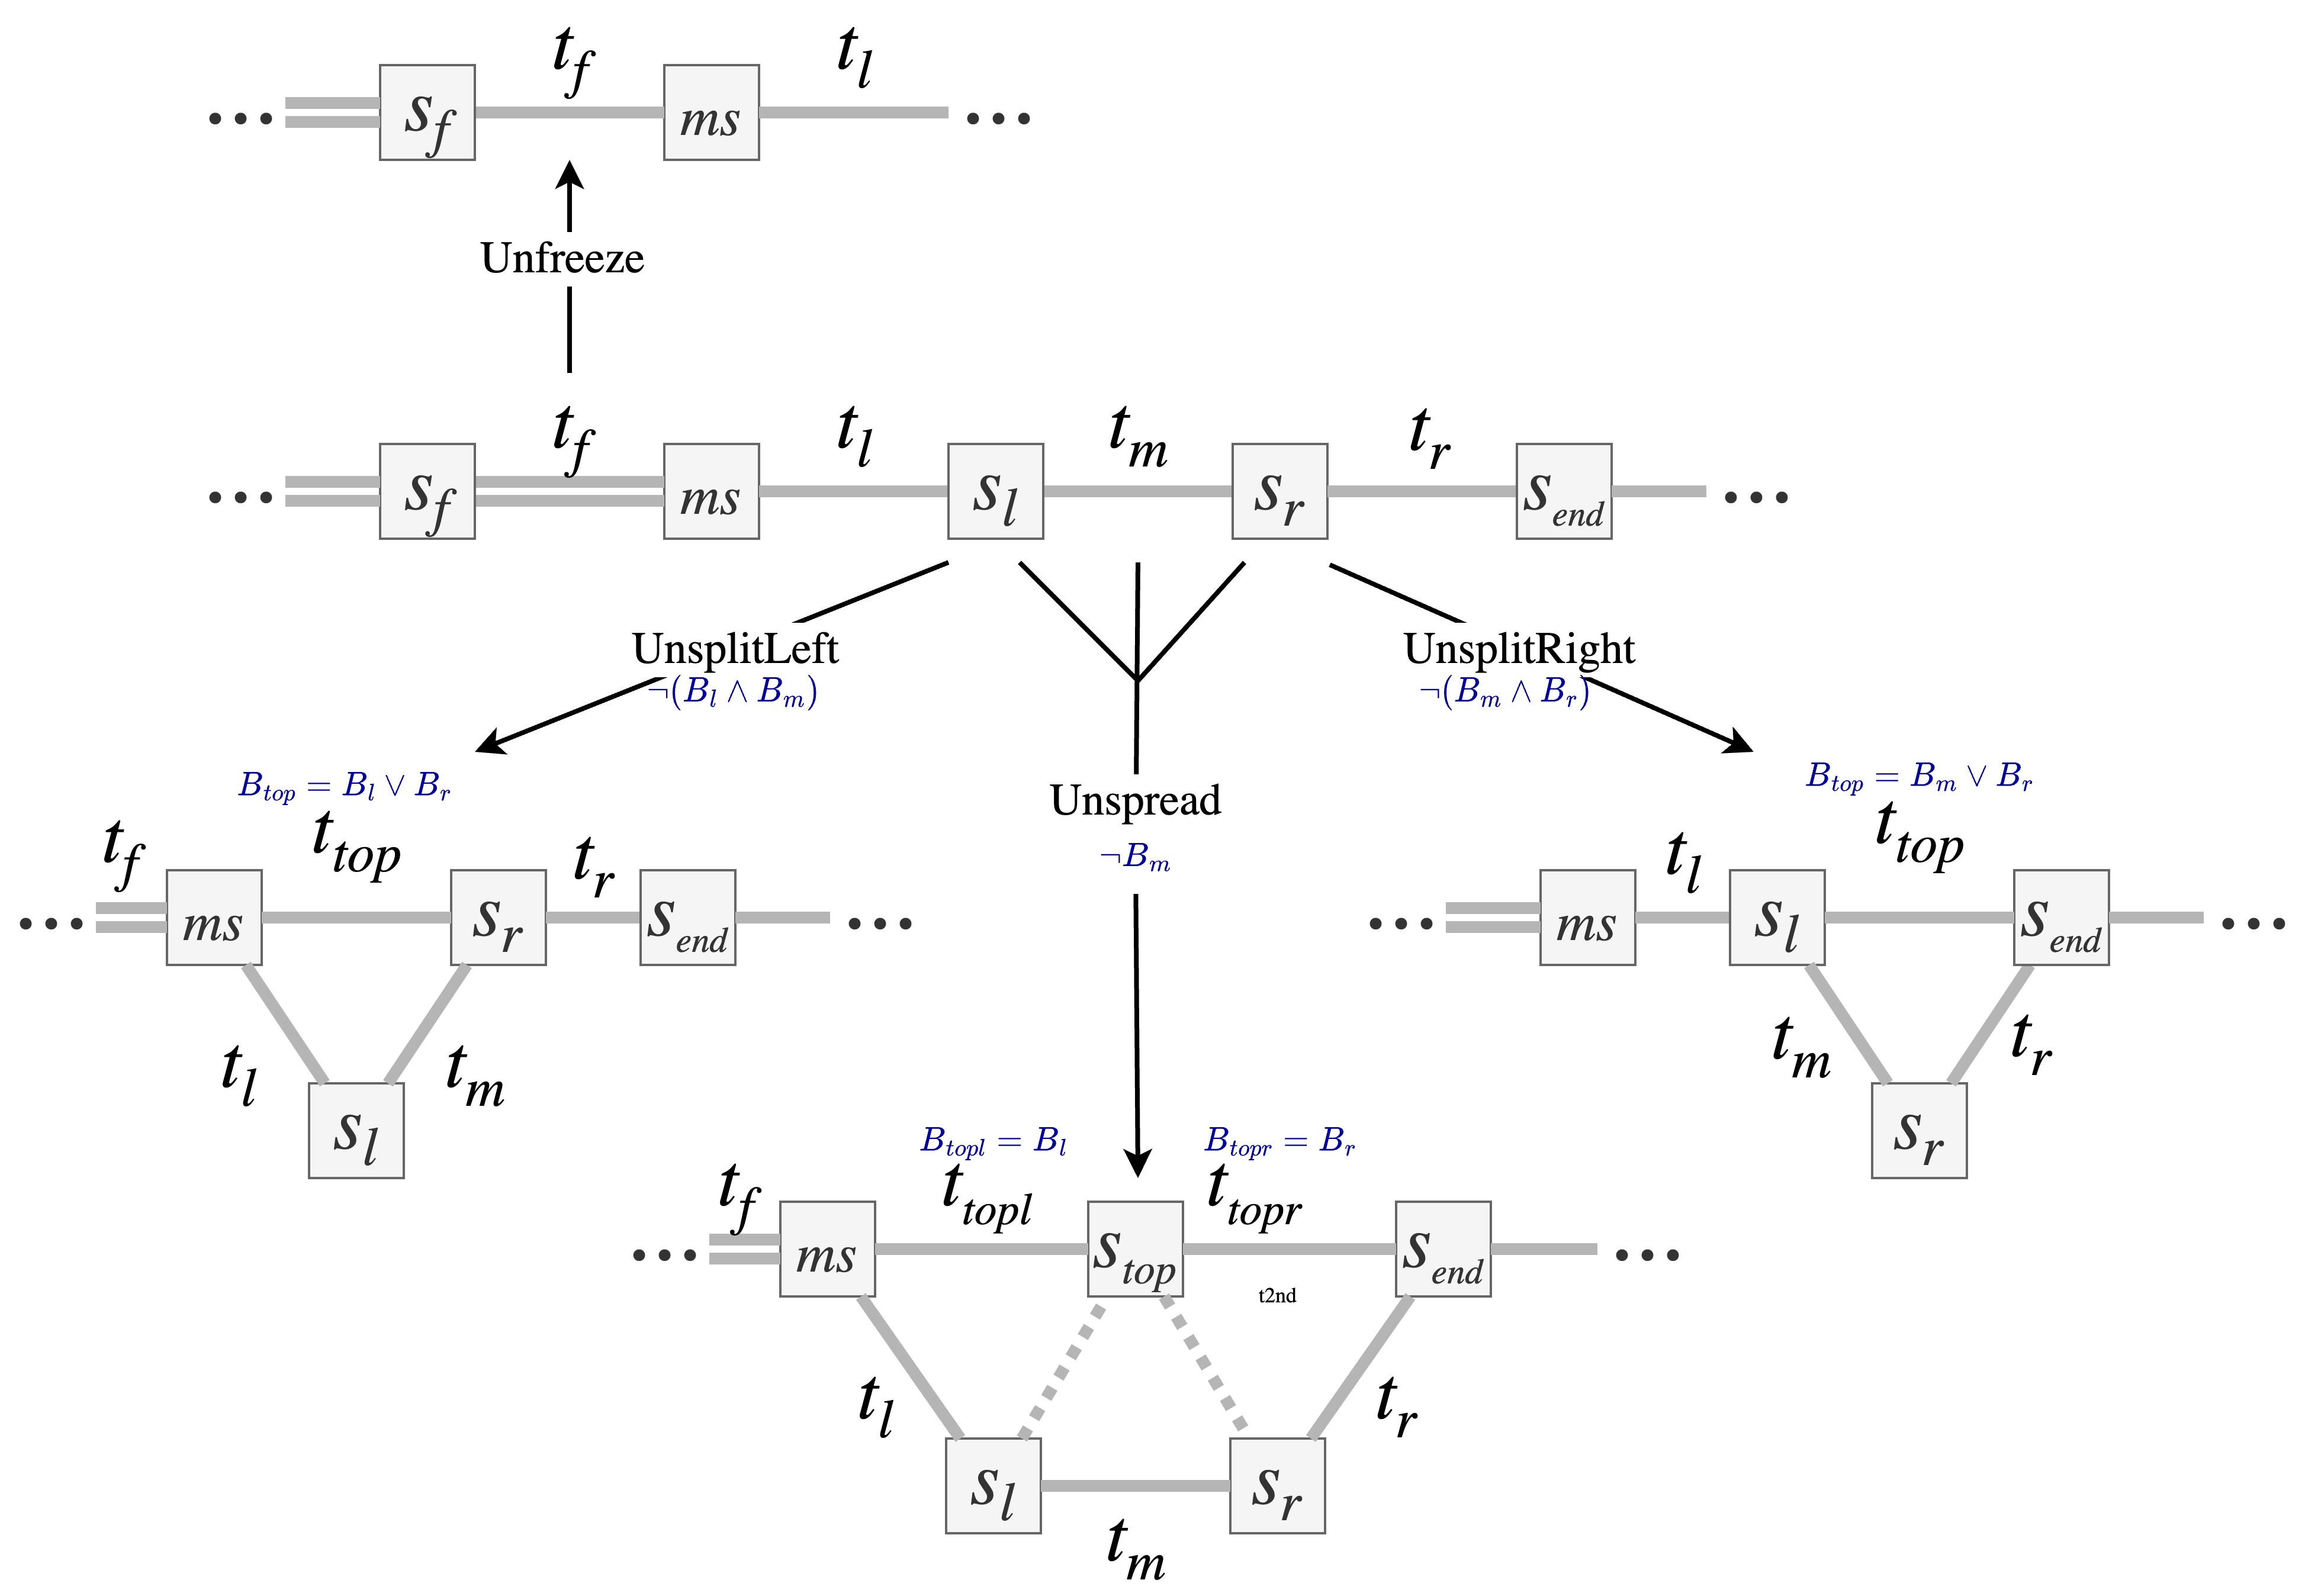
\includegraphics[width=0.85\textwidth]{impl/parseOps}
  \caption{General parse state reductions}
  \label{fig:parseStateOptions}
\end{figure}

\begin{figure}[h]
  \centering
  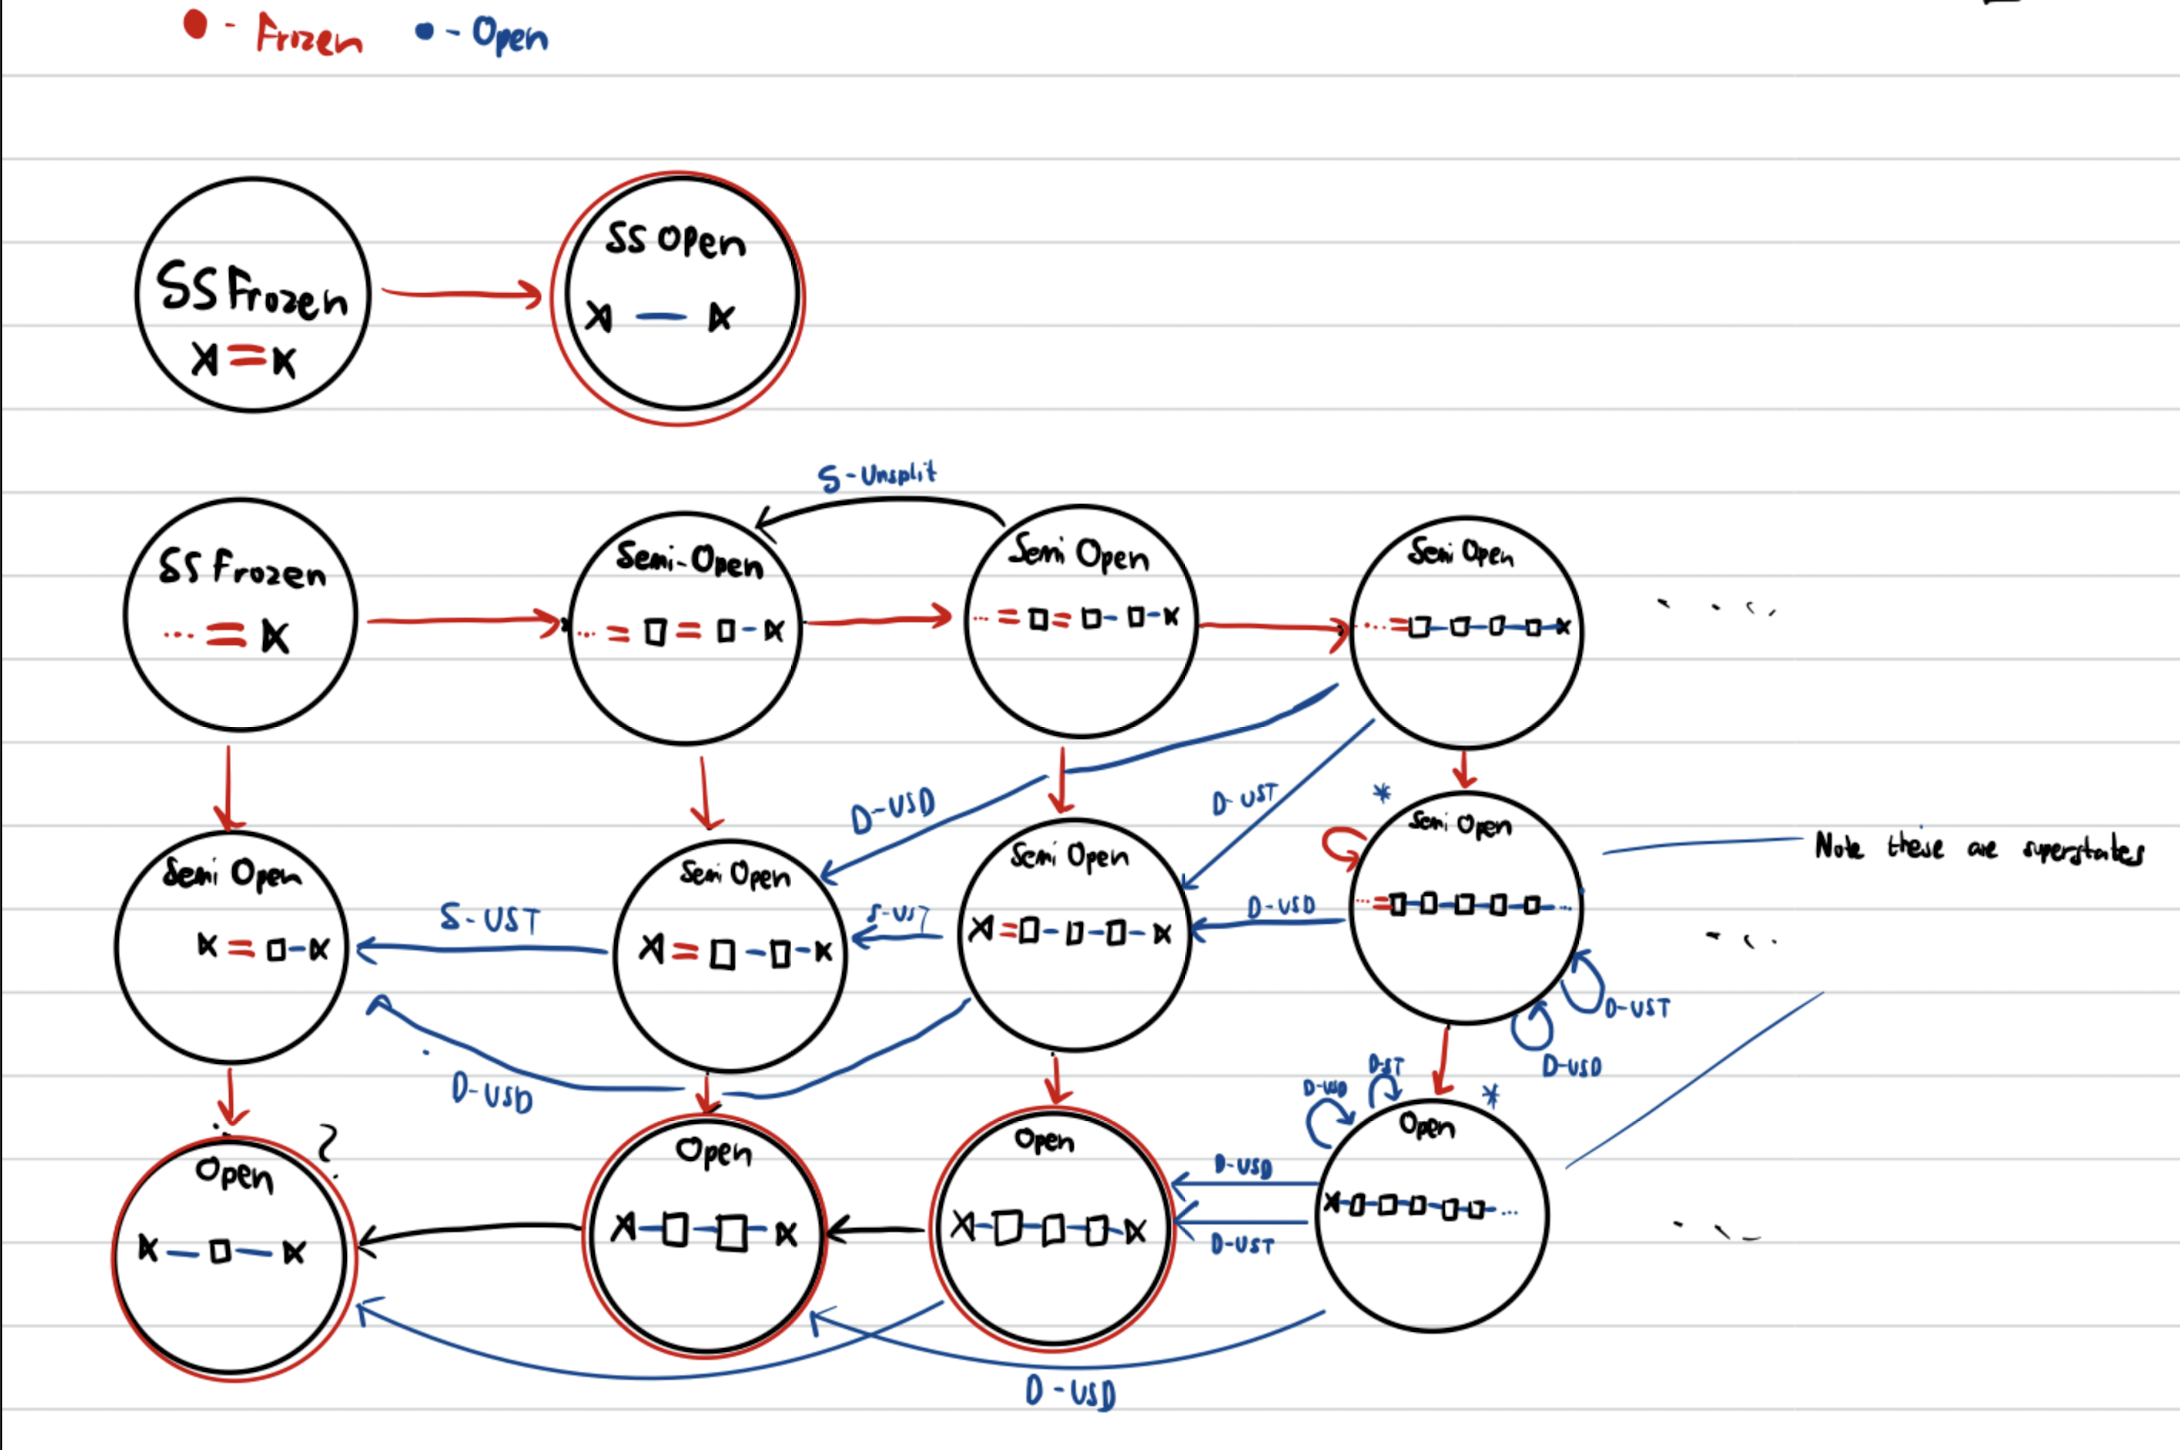
\includegraphics[width=\textwidth]{statetransitions}
  \caption{State Transition diagram}
  \label{fig:statetrans}
\end{figure}

In the state transition diagram (Figure \ref{fig:statetrans}), we see all the possible parse states (Is this actually useful? Maybe for appendix). This was useful for me as it helps to conceptualise how the full parse actually works. The dimensions of this digramm of the search state depends on the length of the piece, and the size of each segment. We can see that there is a process of moving to the right to unfreeze transitions, and moving towards the left during reduction operations. Perhaps some simplification of the diagram would be useful. This transition diagram does not consider segment boundaries.

\FloatBarrier
\section{Baseline implementation}


\subsection{Baseline Reduction}
As a crude baseline we develop two algorithms based on randomly sampling notes for each segment to infer the chord label. 
\par
The pure random sample algorithm simply samples random notes for each segment, and uses those to guess the chord label. This doesn't even consider the notes of the piece, so it's really bad, but provides a useful reference.
\par 
The per segment sample algorithm samples notes from each segment. Could just sample a random number of notes from each segment, or just use all the notes in the segment to predict the most likely chord label. This is reminiscent of using a key-profile model \cite{temperleyBayesianApproachKeyFinding2002} to find local keys.

\FloatBarrier
\subsection{Random Search}
Now we use our implementation of the protovoice parser, but just do a random walk in the tree of partial reductions. By comparing this against the random ample parser, we can get an idea of the utility of the model. We show that this works surprisingly well.

\FloatBarrier
\section{Extension Implementation}

\subsection{Heuristic Design}
Step 1: Design heuristic to be as accurate as possible. I.e the extreme is to consider every possible parse, but for a single piece there can be over $10^{10^{10^{10^{10^{10}}}}}$ different parses. We consider 1 step at a time at first - this still results in needing to choose an operation out of upwards of 30,000,000 options for just a single step.     
\par
First the full piece heuristic parse 
\par
The goal of the heuristic is to find the probability of a reduction. 

\begin{figure}[ht]
  \centering
  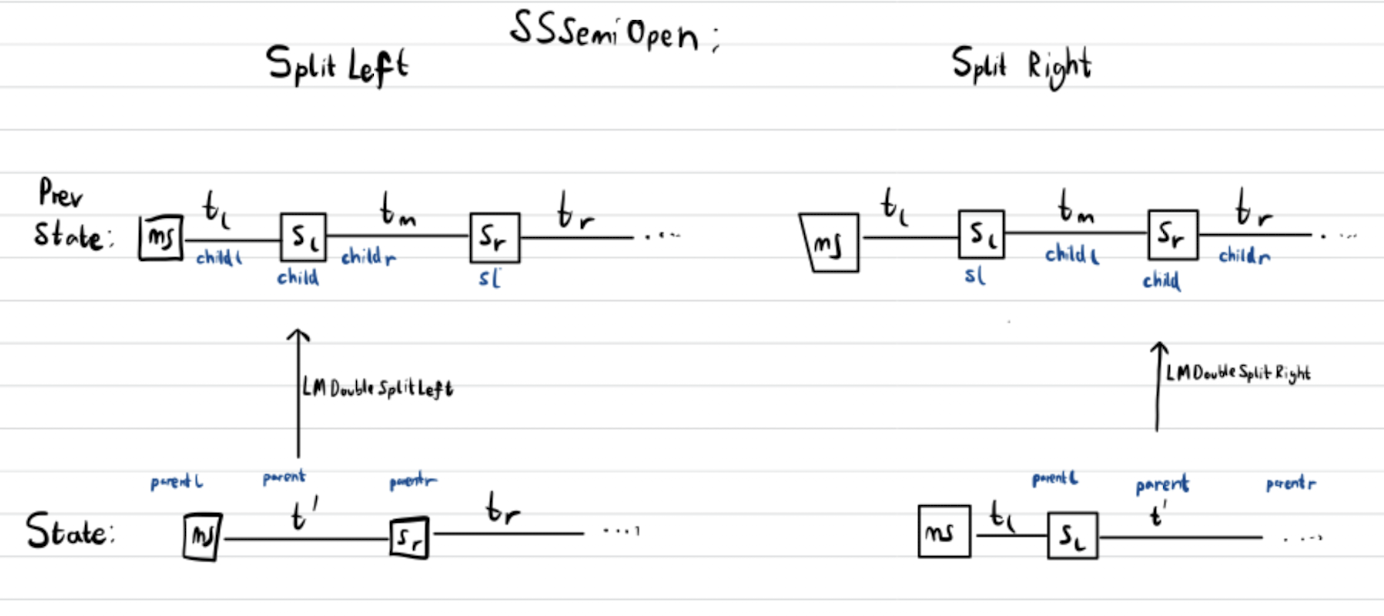
\includegraphics[width=0.7\textwidth]{splitsssemiopen}
  \caption{Split operation}
  \label{fig:splitoperation}
\end{figure}

\FloatBarrier
\subsubsection{Scoring Unsplit Operations}
Consider the Split rule : \[t \to t'_{l}~s'~t'_{r}\]
\par
During a split, each edge in the transition and each node in an adjacent slice can be elaborated by one or more inner operations.
These new edges can be discarded or kept to form the new edge of $t'_l$ and $t'_r$.
\par 
The notes in the child slice $s$ can either have edges connected to the left neighboring slice or right neighbouring slice, or both. I.e for each note in the child slice, it can be a an ornmentation of a previous note, subsequent note, both, or repetition of prev note, subsequent note etc. So we consider the chord tone profiles of the involved slices. 

We first guess the chord type each parent slice. 
\[\theta_l = \mathop{argmax}_{c \in C} P(s_l|c) ~~,~~ \theta_r = \mathop{argmax}_{c \in C} P(s_r|c) '\]

We now consider each edge individually, considering their likelihoods based on the proabilistic model of harmony along with theoretical assumptions. 

\paragraph{Single Sided Operations} 
\begin{itemize}
  \item Right Neighbour (Left Neighbour anagolously)
    \[ x \implies x \to n~~, x,n \in P \]
    \[x \sim \text{Categorical}(\sigma_{ct}^{\theta_l})\]
    \[n \sim \text{Categorical}(\sigma_{or}^{\theta_r})\]
    Find \[P(x,n~|~\theta_l)\]
  \item Right Repeat (Left Repeat anagolously)
    \[ x \implies x \to x~~, x \in P \]
    \[x \sim \text{Categorical}(\sigma_{ct}^{\theta_l})\]
    Find \[P(x~|~\theta_l)\]
\end{itemize}
\paragraph{Two Sided Operations} 
\begin{itemize}
  \item Root Note: This operation is only done once in the original model. In our case we do not need to consider due to segment boundaries.
  \item Full Repeat: 
    \[ x \implies x \to n~~, x,n \in P \]
    \[x \sim \text{Categorical}(\sigma_{ct}^{\theta_l})\]
    \[n \sim \text{Categorical}(\sigma_{or}^{\theta_r})\]
    Find \[P(x,n~|~\theta_l)\]
  \item Left Repeat of Right: 
    \[ x \to y \implies x \to y' \to y \]
    \[y \sim \text{Categorical}(\sigma_{ct}^{\theta_l})\]
    Find \[P(y~|~\theta_l)\]
  \item Full Neighbour:
    \[ x_1 \to x_2 \implies x_1 \to n \to x_2, x \in P \]
    % \[x \sim \text{Categorical}(\sigma_{ct}^{\theta_l})\]
    Find \[P(|~\theta_l,\theta_r)\]
\end{itemize}

\FloatBarrier
\subsubsection{Scoring Unspread Operations}

Consider the Spread rule : \[t_l s_r \to t'_l s_l t'_m s_r t'_r\]
We make the assumption that $s$, $s_l$, \& $s_r$ are all realisations of the same chord. This lines up with the music theorretical basis for this operation in the model(justify).
\par 
Thus we find the most likely chord (optional extension: marginalise over all chords)
\[\theta = \mathop{argmax}_{c \in C} P (s|c)\]
\par 
When then measure the extent to which the parent slics match this chord.

\[p(s_l, s_r| \theta)\]

We can calculate $p(s_l|\theta)$ and $p(s_r|\theta)$ using the multinomial distribution probability density function as described in the preparation chapter.

\FloatBarrier
\subsubsection{Scoring Unfreeze Operations}
We assign 0 cost to unfreeze operations. This means we need to be careful about ensure that we don't just unfreeze the entire piece immediately. Careful construction of the search algorithm can ensure this. More later.

\FloatBarrier
\subsubsection{Full state evalutation}
We need to combine all of these in a fair way. Also the distinction between splits and spreads need to be considred, as they are different operations, the calculations of likelihood may cause an imbalance. All likelihoods are stored in log space.

\FloatBarrier
\subsection{Best-First Search}
Given the heuristic $\mathcal{H}_0$, the first option is to use a greedy search.
We keep unfreeze operations as an option.

We find that the number of operations causes a combinatorial blowup, so the search doesn't end.

Problem of very large slices.\\ 
Segment by segment heuristic parse - avoids the problem, but is slightly hacky. Can we incorprate our knowledge regarding the relative proportion of chord tones and ornaments. Should we allow duplicates of notes in slices? Perhaps we should favour spreads more. 

Always consider a certain number of slices and spreads.

\subsection{Beam Search}
Step 2: Relax the heuristic search in order to reduce runtime/ lower complexity.
\par 
In the case that there are 85,000,000 options, perhaps we should sample the options rather than evaluating all of them. 
\par 
This version of heuristic search should be able to parse full pieces (hopefully), so can be used to compare with the baselines on an entire corpus.
\par 
Beam of size n, with 1 for a freeze, k for spread, n-k-1 

\subsection{Dual Beam Search}
It isn't clear how to determine how we should balance the costs of unspread and unsplit op

\subsection{Stochastic Dual Beam Search}
We propose sampling from the options, increasing the proportion that we ignore dependent on the number of options.

\section{Choosing hyper parameters}


\section{Testing}

\subsection{Unit Tests}

\subsection{Qualitative Tests}
 Throughout the design of the heuristic $H_0$ and the implementation of different search algorithms, a few segments we used as reccuring test examples.

\chapter{Evaluation}
\textit{In this chapter, I provide qualitative and quantitative evaluations of the work completed. I then provide and interpret evidence to show that the success criteria were met.}

\textit{The main questions to answer are as follows:}
\begin{itemize}
  \item \textit{Can the proto-voice model be used to accurately infer chord labels?}
  \item \textit{Can the proto-voice model be used to practically infer chord labels?}
  \item \textit{How well my heuristic search algorithms infer chord labels?}
\end{itemize}

\section{Metrics}
Ambiguity. which metrics exist? discussion.
Accuracy and likelihood.

\section{Harmony Model}

\subsection{Accuracy}
When evaluating using the protovoice model: we assume that we result in only chord tones for each segment. Thus we use the chord tone probabilities to evaluate the prediction. 
\par
When just using a random sample, we have to assume that there is a mixture model of chord tones and ornaments. We use the learnt parameters to determine the distribution.
\par
These two measures of likelihoods are comparable as they are drawn from the same distributions.
\par
We also need to infer chord labels. We can simply choose the chord that is most likely according to our model.
\par 
This gives us two key metrics, likelihood and accuracy.
\par
Could also use a more sophisticated notion of accuracy, using a chord similarity function \cite{humphreyFourTimelyInsights2015}. The {\texttt {mir\_eval}} package provides a plethora of metrics to compare chord label predictions \cite{raffelMirEvalTransparent2014}. 

\subsection{Sensitivity Analysis}

\subsection{Qualitative Analysis}

\section{Baseline Algorithms}
Reminder of what the search is actually doing. 

Things to note
\begin{itemize}
  \item The fact that segmentation is known ahead of time provides a great deal of information \cite{gothamWhatIfWhen2021}
  \item So we use comparisons between the random sample from each segment algorithm and the random parse algorithm to see if the use of the grammar provides an advantage over just sampling the notes directly, without looking at relations between notes.
  \item Then we want a heuristic search algorithm that considers each option exhaustively and finds the best local option. This is too computationally expensive to be used for whole pieces. 
  \item Given there can be millions of possible next states in the search, we need to look at different strategies to avoid searching through them all. E.g just sample states. 
  \item Sensitivity Analysis for the heuristic search is useful for the evaluation. Explore how robust it is to handcrafted attacks/ different types of passages.
  \item Could evaluate by segments instead of pieces. 
\end{itemize}

\section{Extension Algorithms}

\subsection{Accuracy}

\subsection{Scalability}

\subsection{Qualitative Analysis}

\section{Success Criteria}

I've shown that i met success criteria x by this analysiss. etc.

\section{Limitations}

I'm solving:

\begin{equation}
    \hat L &= \argmax_L\left(p(S|L)\right) 
\end{equation}

But I could be solving:

\begin{equation}
    \hat L &= \argmax_L\left(p(S|L)p(L)\right) 
    % \underbrace{P(L)}_\text{prior}
\end{equation}

In which case:

To compute the conditional probability $p(L|S)$, we use Bayes' theorem:
\begin{equation}
  p(L|S) = \frac{p(S|L)~p(L)}{P(S)}
  \label{eq:lgivenS}
\end{equation}
Finding the most likely sequence of labels is found using:
\begin{equation}
  \argmax_L \left(\underbrace{p(S|L)}_{\text{likelihood}}~\underbrace{p(L)}_{\text{prior}}\right)
  \label{eq:lgivenSBayes}
\end{equation}

The prior probability of a chord sequence $p(L)$ can be learned from a labeled dataset of chord sequences, and the likelihood can be found using a probabilistic harmony model. The likelihood $p(S|L)$ can be found using 

This would be better, but was beyond the scope of the project.

%%%%%%%%%%%%%%%%%%%%%%%%%%%%%%%%%%%%%%%%%%%%%%%%%%%%%%%%%%%%%%%%%%%%%
% Conclusions
%%%%%%%%%%%%%%%%%%%%%%%%%%%%%%%%%%%%%%%%%%%%%%%%%%%%%%%%%%%%%%%%%%%%%

\chapter{Conclusions}
\textit{In this chapter, I first discuss the success achieved by the project then offer a reflection on lessons learned. Finally, I consider the directions in which there is potential for future work.}
\section{Achievements}

\section{Lessons learned}

\section{Future Work}



%%%%%%%%%%%%%%%%%%%%%%%%%%%%%%%%%%%%%%%%%%%%%%%%%%%%%%%%%%%%%%%%%%%%%
% the bibliography
%%%%%%%%%%%%%%%%%%%%%%%%%%%%%%%%%%%%%%%%%%%%%%%%%%%%%%%%%%%%%%%%%%%%%
\addcontentsline{toc}{chapter}{Bibliography}

\nocite{*}
% \addbibresource{Disseration.bib}
\bibliography{Dissertation}


%%%%%%%%%%%%%%%%%%%%%%%%%%%%%%%%%%%%%%%%%%%%%%%%%%%%%%%%%%%%%%%%%%%%%
% the appendices
%%%%%%%%%%%%%%%%%%%%%%%%%%%%%%%%%%%%%%%%%%%%%%%%%%%%%%%%%%%%%%%%%%%%%

\appendix

\chapter{Additional Information}

% \section{metadata.tex}
% {\scriptsize\verbatiminput{metadata.tex}}
%
% \section{main.tex}
% {\scriptsize\verbatiminput{main.tex}}
%
% \section{proposal.tex}
% {\scriptsize\verbatiminput{proposal.tex}}
%
% \chapter{Makefile}
%
% \section{makefile}\label{makefile}
% {\scriptsize\verbatiminput{makefile.txt}}
%
% \section{refs.bib}
% {\scriptsize\verbatiminput{refs.bib}}


\chapter{Project Proposal}
\label{chap:proposal}
% Note: this file can be compiled on its own, but is also included by
% diss.tex (using the docmute.sty package to ignore the preamble)
\documentclass[12pt,a4paper,twoside]{article}
\usepackage[pdfborder={0 0 0}]{hyperref}
\usepackage[margin=25mm]{geometry}
\usepackage{graphicx}
\usepackage{parskip}
\begin{document}

\begin{center}
\Large
Computer Science Tripos -- Part II -- Project Proposal\\[4mm]
\LARGE
How to write a dissertation in \LaTeX\\[4mm]

\large
M.~Richards, St John's College

Originator: Dr M.~Richards

14 October 2011
\end{center}

\vspace{5mm}

\textbf{Project Supervisor:} Dr M.~Richards

\textbf{Director of Studies:} Dr M.~Richards

\textbf{Project Overseers:} Dr F.~H.~King  \& Dr A.~W.~Moore

% Main document

\section*{Introduction}

\emph{The problem to be addressed.}

Many students write their CST dissertations in \LaTeX\ -- and spend a
fair amount of time learning just how to do that. The purpose of this
project is to write a demonstration dissertation that provides
a starting point to show how it is done.

This core proposal document will be augmented by a separately-printed
cover sheet at the front and a resource form at the end. Additional
sheets for risk assessment and human resources may also need to be
included.

This document will elaborate much of the material that is summarised on
the additional sheets.

\section*{Starting point}

\emph{Describe existing state of the art, previous work in this area,
  libraries and databases to be used. Describe the state of any
  existing codebase that is to be built on.}

I am already able to write prose using the English language. I have an
online dictionary, etc.

\section*{Resources required}

\emph{A note of the resources required and confirmation of access.}

For this project I shall mainly use my own quad-core computer that
runs Fedora Linux. Backup will be to github and/or to an SVN
repository on an external hard disk that is dumped to writable CD/DVD
media. I have another similar computer to hand should my main machine
suddenly fail. I require no other special resources.

\section*{Work to be done}

\emph{Describe the technical work.}

The project breaks down into the following sub-projects:

\begin{enumerate}

\item The construction of a skeleton dissertation with the required
  structure. This involves writing the Makefile and making dummy
  files for the title page, the proforma, chapters 1 to 5, the
  appendices and the proposal.

\item Filling in the details required in the cover page and proforma.

\item Writing the contents of chapters 1 to 5, including examples of
  common \LaTeX\ constructs.

\item Adding a example of how to use floating figures and ``encapsulated
  PostScript'' or PDF diagrams.

\end{enumerate}

\section*{Success citeria}

\emph{Describe what you expect to be able to demonstrate at the
end of the project and how you are going to evaluate your achievement.}

The project will be a success if I have a completed dissertation with
the correct chapter titles and I have achieved my other success
criteria, which are to blah \ldots


\section*{Possible extensions}

{\em Potential further envisaged evaluation metrics or extensions.}

If I achieve my main result early I shall try the following
alternative experiment or method of evaluation \ldots


\section*{Timetable}

\emph{A workplan of perhaps ten or so two-week work-packages,
as well as milestones to be achieved along the way. Provide a
target date for each milestone.}

Planned starting date is 16/10/2011.

\begin{enumerate}

\item \textbf{Michaelmas weeks 2--4} Learn to use X. Read book Y. Read papers Z.

\item \textbf{Michaelmas weeks 5--6} Do preliminary test of Q.

\item \textbf{Michaelmas weeks 7--8} Start implementation of main task A.

\item \textbf{Michaelmas vacation} Finish A and start main task B.

\item \textbf{Lent weeks 0--2} Write progress report. Generate corpus of
  test examples. Finish task B.

\item \textbf{Lent weeks 3--5} Run main experiments and achieve working project.

\item \textbf{Lent weeks 6--8} Second main deliverable here.

\item \textbf{Easter vacation:} Extensions and writing dissertation main
  chapters.

\item \textbf{Easter term 0--2:}  Further evaluation and complete dissertation.

\item \textbf{Easter term 3:} Proof reading and then an early submission
  so as to concentrate on examination revision.

\end{enumerate}

\end{document}

\end{document}
